\chapter{Strategic Classification for Non-uniform Preferences using Penalty Labels and Randomisation}
\label{ch:strat_class}

Strategic classification is the problem of classifying feature vectors that can be manipulated at the testing phase of the classifier. The classifier aims for its decision rule to be robust against strategic manipulation and also be efficiently learnable. In this chapter, we present two main ideas for the classifier to achieve this goal. The first idea is to enrich the classifier's decision-making capabilities in two ways: ignoring feature vectors and making randomized decisions. This approach helps the classifier classify more feature vectors correctly by limiting the sender's options for manipulation. The second idea is to use the strategic structure of the problem during learning. This approach, in certain contexts, can simplify the learning process. Combining these ideas, we propose and compare two learning algorithms, Vanilla ERM and Strategy-aware ERM, and provide a heuristic for selecting the one that yields a classifier both robust to strategic manipulation and efficiently learnable.

\section{Introduction}
\label{sec:Introduction}
Consider the following classification situation. A university assigns students to various programs based on their scores in an aptitude test using a decision rule that maps scores to programs. For example, one such rule could be to assign the Physics program to students who have scored well in the physics section of the exam, regardless of their total score. For transparency, the university must declare its decision rule before the students write the exam. Every student taking the exam has a \textit{true aptitude} corresponding it with a \textit{true program}.
However, the students may have preferences for programs that may differ from their true programs. Knowing the decision rule, they can seek external help, such as coaching, to improve their scores, incurring some costs for such assistance. 
Now suppose the university offers two related programs (say theoretical and experimental physics programs), where the students with an aptitude in one program may prefer the other program and, therefore, prepare for the entrance exam accordingly. The university aims to create a question paper for the entrance exam  in such a manner as to assign the maximum number of students to their true programs. The challenge is that the university cannot measure the true aptitude of a student and must rely on the exam scores, i.e., its \textit{demonstrated aptitude}, to assign the program. Moreover, the university does not know the \textit{true function} (which maps true aptitude to a true program) and must learn it from past data.

The university admission problem is an example of a \textit{strategic} classification problem. The strategic classification problem extends the classification problem to the regime where, during the classifier's testing phase, a strategic data sender can manipulate feature vectors to obtain a preferred label while incurring some cost. A non-strategic or \textit{naive classifier} places the decision boundary precisely at the class boundary. Since this classifier's decision rule is known to the strategic sender, it is prone to manipulation. A \textit{strategic classifier} is robust to such manipulation and, in general, differs non-trivially from the naive classifier.

Existing works on the strategic classification problem typically assume that the sender has a uniform preference for the labels (e.g., \cite{hardt2016strategic}). The standard example of this setting is the email classification problem, where the strategic sender prefers the non-spam label over the spam label, irrespective of the underlying email content. The strategic classifier for this case is the one that shifts the decision boundary into the \textit{non-spam} region of the feature space, thereby making the criterion for classification as the non-spam label more stringent.

This chapter considers a binary classification problem where the strategic sender has a possibly non-uniform preference for labels, as illustrated in the above example for admission to theoretical and experimental physics programs. This assumption poses a new challenge as preferred feature space for one class overlaps with the space not preferred by the other. In particular, the structure of the strategic classifier obtained by \cite{hardt2016strategic} no longer holds without a universally preferred label.
The problem of constructing a strategic classifier with non-uniform preferences results in two subproblems: a \textit{decision problem} and a \textit{learning problem}. In the decision problem, the university knows the \textit{true function} (map between the true aptitude and the true program) and has to calculate the strategic classifier from it. In the learning problem, the university does not know the true function and has to learn the strategic classifier from a finite sample of the true function.

Our main findings are that classification performance improves significantly when the classifier is either allowed to make randomized decisions or allowed to \textit{not} classify certain feature vectors. Moreover, in certain problem instances, particularly those involving complex hypothesis classes, learning can be made easier by incorporating the sender's strategic behaviour in the classifier's learning phase.

\subsection{Contributions}

We adopt a game theoretic viewpoint for our analysis. We model the binary classification problem with non-uniform preferences as a screening game\footnote{In a screening game, the receiver commits to a strategy first; the sender then observes this commitment and chooses a strategy in response, after which the receiver plays the committed strategy.} between a sender and a receiver (classifier), with the receiver as the leader. The sender wants to maximize the difference between its utility and its cost and the receiver wants to maximize the probability of correctly classifying the feature vectors. The strategic classifier corresponds to the receiver's Stackelberg equilibrium strategy. For most of our results, we work with a scalar feature space. We show that under certain assumptions, the problem with the vector feature space with a linear class boundary can be reduced to the problem we consider. 

We introduce two main ideas. The first is to expand the classifier's capabilities in two ways. One way is by introducing a new penalty label $\Delta$, by which means the receiver ignores a feature vector assigned to this label. From the sender's perspective, this situation is equivalent to receiving a $-\infty$ utility for the label $\Delta$. In the context of university admission problems, the student is the sender, and the university is the receiver. The exam paper comprises of a subset of questions from a question bank, with the requirement that the student has to attempt exactly one question. The university assigns a label to each question in the exam paper with the implication that a student who correctly answers that question gets assigned that label or program. Assignment of label $\Delta$ to a question amounts to \textit{dropping} that question from the exam paper. This approach is in stark contrast to the uniform preference case, where \textit{all} the questions in the question bank are included in the question paper, and only \textit{cut-off marks} for the preferred program are increased.
Ignoring feature vectors can also be considered a generalization of feature selection.

Another way to expand the classifier's action set is by allowing randomized classification. In the university admission problem, this is analogous to saying that solving a particular question is correlated (but not with certainty) with admission to a specific program. These ideas for expanding the classifier's action set are motivated from mechanism design, where penalties influence a strategic sender's behavior, and game theory, where randomization allows for richer outcomes.

The second main idea involves incorporating the underlying game-theoretic structure of the problem by modifying the hypothesis class used for learning. Learning from the original hypothesis class will be inefficient if the university's inductive bias does not consider students' strategic nature. We show that incorporating the game's strategic structure through hypothesis class modification can make an unlearnable hypothesis class learnable.

Using these two ideas, we address the decision and learning problems of strategic classification in the scalar feature space setting. For the decision problem, our first finding is that a deterministic strategic classifier using a penalty label makes fewer classification errors than any classifier that does not use a penalty label, at least strictly fewer errors in some instances of the problem. 
With probability $1 - \delta$ (where we will write this in sections), a stochastic strategic classifier makes fewer errors than any deterministic classifier, including those that use a penalty label, and at least strictly fewer errors than a classifier with a penalty label in some instances of the problem.

However, the stochastic classifier uses only randomization on the original label set; using the penalty label does not increase its accuracy. Nonetheless, the penalty label becomes relevant when it is constrained to use a deterministic strategic classifier, a common situation encountered in real-life applications. Hence, the penalty label can be thought of as partially compensating the classifier for the absence of randomization.

The classifier described above assigns the label $\Delta$ to feature vectors near the class boundary. Indeed, multiple such classifiers exist, all with the same classification error, but they differ in the following three aspects.
The first aspect is classifier complexity, measured by the number of decision boundaries. A decision boundary is a feature vector at which the classifier changes its assigned label. Thus, the number of decision boundaries corresponds to the number of times the classifier switches labels as the feature vector varies. We show that classifiers with fewer decision boundaries are easier to learn due to their lower Vapnik--Chervonenkis (VC) dimension.
The second aspect is classifier fairness, which refers to fair distribution of errors across classes. If in addition to classification performance, fairness is also in consideration, then the receiver can pick among the many classification rules, the one which proportionately distributes the error across classes. The third aspect is the sender's payoff under a strategic classifier. This aspect becomes relevant if a sender can opt-out and obtain a reservation payoff. Thus, a receiver may select a classifier that gives the sender a payoff higher than its reservation payoff. Although we work with scalar features, our problem suffices to demonstrate the structural aspects of strategic classification and the importance of a penalty label. Moreover, in many university admission problems like those we consider, the final admission decision has to be done based on a single scalar score, whereby the scalar problem is practically relevant.

We introduce two new algorithms called vanilla ERM and strategy-aware ERM to address the learning problem. In vanilla ERM, the classifier first uses ERM to learn the true function from the original hypothesis class. The decision problem is then applied to the learned hypothesis. In the strategy-aware ERM approach, the hypothesis class is modified to incorporate the underlying game-theoretic structure. This modification involves a two-step process. First, each hypothesis in the original class is replaced with its corresponding strategic classifier, which is obtained by applying the decision problem to each hypothesis. Second, the strategic classifier obtained in the previous step is further replaced with a new hypothesis, formed by composing the strategic classifier with the sender’s worst-case best response. The classifier then uses the Empirical Risk Minimization (ERM) algorithm to learn from this modified hypothesis class. What makes strategy-aware ERM novel is its ability to transform an otherwise unlearnable problem into a learnable one. We show that there exist hypothesis classes that are unlearnable under vanilla ERM but become learnable with strategy-aware ERM, illustrating how incorporating game-theoretic structure can fundamentally improve learnability.

While strategy-aware ERM can learn from a broader range of hypothesis classes, its advantage in the ease of learning over vanilla ERM only sometimes holds. This ease of learning is controlled by the VC dimension of the hypothesis class, which in turn determines the sample complexity in PAC learning. The comparison, therefore, becomes context-dependent if a hypothesis class is learnable via vanilla ERM. We provide a heuristic argument that strategy-aware ERM generally makes learning easier if the original hypothesis class is too complex, as it can reduce the effective VC dimension. On the other hand, vanilla ERM proves more efficient if the original hypothesis class is simple. We show this with the help of an example. A formal result, even for scalar features, remains elusive.

\subsection{Related Work}
This chapter contributes to the literature on strategic classification and learning in the presence of strategic agents~\cite{bruckner2011stackelberg,ghalme2021strategic,bechavod2022information,cohen2024bayesian,jagadeesan2021alternative,dalvi2004adversarial}, where interactions are commonly formulated as games between a strategic sender and a classifier. We model this interaction as a sender--receiver screening game and introduce a penalty label that expands the receiver's strategy space, giving rise to equilibrium strategies robust against the sender's manipulation. Preliminary versions of the results in this chapter appeared in the conference papers~\cite{singh22strategic,singh2024optimal}. This chapter is derived from our manuscript~\cite{singh2025strategic}. To the best of our knowledge, the setting of strategic classification under non-uniform preferences with penalty labels has not been previously studied, and was first explored in our work~\cite{singh2025strategic}.

Works such as \cite{hardt2016strategic,cullina2018pac,zhang2021incentive,sundaram2021pac} consider the impact of a strategic sender on the PAC learnability of the hypothesis class. In \cite{hardt2016strategic,cullina2018pac,zhang2021incentive}, the sender is assumed to have a uniform preference for positive labels, whereas in \cite{sundaram2021pac}, the sender is assumed to have a non-uniform preference for labels for each feature vector. In \cite{hardt2016strategic,cullina2018pac,sundaram2021pac}, strategic manipulation incurs a cost, whereas in \cite{zhang2021incentive}, strategic manipulation does not incur a cost. The works \cite{hardt2016strategic,cullina2018pac,zhang2021incentive,sundaram2021pac} do not explicitly utilize the underlying sender-receiver game in the learning process. The learning process in these works can be equivalently described as using the ERM algorithm to optimize over a modified hypothesis class, obtained by replacing each hypothesis with the composition of the hypothesis and the sender's best response to that hypothesis. In contrast, in this chapter, the sender has a non-uniform preference over labels for each feature vector, and the structure of this preference differs from that in \cite{sundaram2021pac}. Furthermore, in this chapter, there is a cost incurred for modifying a feature vector. We explicitly make use of the underlying sender-receiver game in the learning process by allowing the ERM algorithm to optimize over a modified hypothesis class, which is obtained by replacing each hypothesis with its corresponding Stackelberg equilibrium composed with the sender's best response.

There are other interesting formulations of the problem that we do not consider in this chapter. For instance, some research explores scenarios where the sender lacks knowledge of the classifier. Notable works in this area include \cite{ghalme2021strategic}, \cite{bechavod2022information}, and \cite{cohen2024bayesian}. Additionally, other studies introduce more structure to the sender by incorporating user types, as seen in \cite{jagadeesan2021alternative} and \cite{levanon2022generalized}.

Finally, the social welfare implications of strategic classification have been explored in works such as \cite{milli2019social}, which analyze the social costs imposed on the sender. In this chapter, we briefly address related issues such as fairness and participation constraints in Section~\ref{subsec:Other equilibria}.


\section{Problem Formulation}\label{sec:Problem formulation}
In this section, we formulate the strategic classification problem. Recall that in strategic classification, the sender can alter the feature vector at a cost during the classifier's testing phase to obtain a preferred label.

We formalize the strategic classification problem within this framework. Let $\cg{X}$ be the set of feature vectors; for simplicity we take $\cg{X}:= [0,1]$. Consider an abstract probability space and let $X$ be a $\cg{X}$-valued random variable defined on that space. Let $\cg{L}(X)$ denote the probability law of $X$ on  $\cg{X}$. Let $\fk{D}$ be the collection of laws of $X$ such that the corresponding cumulative distribution function, denoted as $\psi(\cdots)$, is differentiable and has a differentiable inverse except at finitely many points.
We use $D$ to represent an element of $\fk{D}$. Let $\cg{Y} :=\{-,+\}$ be the set of labels. Let $h: \cg{X} \rightarrow \cg{Y}$ be a \textit{true function} that maps each feature $x \in \cg{X}$ to its corresponding \textit{true label} $y \in \cg{Y}$. We assume the true function to be given by
\begin{equation}\label{eqn:True function}
	h(x) := \begin{cases}
		\minus, & x \in [0,\h] \\
		\plus, & x \in (\h,1]
	\end{cases},
\end{equation}
where $0 \leq \h \leq 1$. We refer to $\h$ as the class boundary. We call a label a \textit{majority class} label if the corresponding feature vectors whose true label is the said label has a probability (under probability law $D \in \fk{D}$) greater than or equal to half. The other label is called the \textit{minority label}.

We model the strategic classification problem  as a game between two players, a sender and a receiver (classifier), who engage in a sender-receiver game with the receiver acting as the leader. The receiver is interested in correctly classifying  the feature vectors, whereas the sender is interested in obtaining a preferred label for each feature vector by potentially misreporting the feature vector. The gameplay proceeds as follows. The sender observes a realized feature vector $x\in \cg{X}$ drawn according to a probability law $D \in \fk{D}$ and modifies it to $s(x) \in \cg{X}$ according to a rule $s$. It then communicates $s(x)$ to the receiver, who then classifies it with a label $r(s(x))$ according to a rule $r$.

The sender's strategy set for modifying feature vectors is given by
\begin{equation}\label{eqn:Sender's strategy space}
	\mathsf{S} := \{s \;|\; s: \cg{X} \rightarrow \cg{X} \}
\end{equation}
and the receiver's strategy set for classification is given by
\begin{equation}\label{eqn:Receiver's strategy space}
	\msf{R} := \{r\;|\; r:\cg{X} \rightarrow \cg{Y} \cup \Delta\}.
\end{equation}
Here, label $\Delta$ is an additional label, which we call the penalty label, whose interpretation will be provided later in this section. We refer to the set $\{x: r(x) = \Delta\}$ of feature vectors with label $\Delta$ as the $\Delta$-region.

We analyze the above game as a screening game;
the receiver first commits a strategy $r \in \msf{R}$, and then the sender, who knows the committed strategy, plays a strategy $s \in \msf{S}$, and finally the receiver plays his committed strategy $r$. Notice the asymmetry in the role of the sender and the receiver. The receiver can perform classification but cannot access the private information of the sender (the feature vector $x$). In contrast, the sender has access to private information but can not do classification and has to depend on the receiver to get his (preferred) label.

The sender's preference for the label for each feature vector is represented by a utility function $U: (\cg{Y} \cup \Delta) \times \cg{X} \rightarrow \R \cup \{-\infty\}$. We assume it to be  given by

\begin{equation}\label{eqn:Utility}
	U(y,x) := \begin{cases}
		\up & x \in [0,\h], y = \plus \\
		\um & x \in (\h,1], y = \minus \\
		0 & y = h(x)\\
		-\infty & y = \Delta
	\end{cases},
\end{equation}\index{Penalty label|textbf}
where $\um,\up \in \R.$
Note that our choice of the utility function is more general than the one considered in \cite{hardt2016strategic}, as it allows the sender to have a non-uniform preference for labels at each feature vector, making the receiver's task more difficult. The cost incurred by the sender when modifying $x$ to $x'$ is given by $C(x,x') = |\phi(x') - \phi(x)|$, where the function $\phi: \cg{X} \rightarrow [0,1]$, called cost kernel\index{Cost kernel|textbf}, is a strictly monotonically increasing, invertible,   continuous function such that $\phi(0) = 0$ and $\phi(1)  = 1$.

In the strategic classification problem, for a strategy $(r,s)$ and a feature vector $x \in \cg{X}$, the sender's payoff at $x$ is given by
\begin{equation}
	\senpayoff(x;r,s):= U(r(s(x)),x) - C(s(x),x).
\end{equation}
For a probability law $D \in \fk{D}$ on $\cg{X}$, the sender overall payoff, which is wants to maximize, is given by
\begin{equation}\label{eqn:Sender's payoff}
	\mathcal{U}(r,s) :=\E_{x \sim D}[\senpayoff(x;r,s)].
\end{equation}
For a strategy $(r,s)$ and a function $f: \cg{X} \rightarrow \cg{Y}$, the error set $E(r,s;f)$ be defined as
\begin{equation}\label{eqn:error set}
    E(r,s;f  ) := \{x \in \cg{X}: r(s(x)) \neq f(x).\}
\end{equation}
 For a probability law $D \in \fk{D}$ with a differentiable distribution function $\psi(x)$,
the receiver's error, which it wants to minimize, is given by
\begin{equation}\label{eqn:Average loss}
	\cg{E}(r,s;h,D) = D(E(r,s;h)) = \int_0^1 \mathbbm{1}_{E(r,s;h)}{\psi'}(x)dx.
\end{equation}
Here $\mathbbm{1}_A$ denotes an indicator function on the set $A$ and
$\psi'(x) = \frac{d\psi(x)}{dx}$


\begin{rem}
	We assume the set $\{x \in \cg{X}| r(s(x)) \neq h(x)\}$ is measurable w.r.t. $D$.
\end{rem}

\subsection{Interpretation of the penalty label}
We now provide an interpretation of the penalty label. If the receiver classifies a feature vector $x$ as  $\Delta$, i.e., $r(x) = \Delta$, then the receiver ignores the feature vector $x$. We assume that ignoring $x$ results in an error for the receiver. From \eqref{eqn:Utility}, $U(\Delta) = -\infty$, which implies that the penalty label is the least preferred label for the sender.

The receiver can exploit this fact to improve its classification accuracy. This property, where the receiver ignores certain feature vectors, is one of the novel contributions of this chapter. It is not considered in \cite{hardt2016strategic}, and we later show that it helps the receiver reduce overall misclassification.

\subsection{Solution concept}
We now describe the solution concept of our problem. For a given receiver strategy $r$, the best response strategies of the sender are defined as follows.

\begin{defn}\label{defn:Best response}\index{Best response|textbf} Let $r$ be a receiver strategy. Let $B(r)$ be the set of sender strategies $s$ which satisfy
	\begin{equation*}
		s(x) \in \arg\max_{x' \in \cg{X}} U(r(x'),x) - C(x',x) \; \forall x \in \cg{X}.
	\end{equation*}
	The set $B(r)$ is called the best response set.
\end{defn}

There can be multiple best responses. We assume that the receiver anticipates that the sender will play a worst-case best response strategy, which is defined as follows.
\begin{defn}[Worst case best response]\label{def:Worst case best response}\index{Worst-case best response|textbf}\index{Best response!worst-case|textbf}
	A sender strategy $s_r$ is called a worst-case best response to a receiver strategy $r$ if
	\begin{equation*}
		\begin{aligned}
			&s_r \in  \arg \min_{s' \in B(r)}D(\{x:r(s'(x)) = h(x)\}) &\text{and}\\ &\{x:r(s'(x)) = h(x)\} \not\subset \{x:r(s_r(x)) = h(x)\} &\text{for all } s' \in B(r).
\end{aligned}
\end{equation*}

\end{defn}
\begin{rem}\label{rem:disclaimer}
	We always assume the receiver's strategy set $\mathsf{R}$ is such that $B(r)$ is non-empty and $s_r$ is well defined.
\end{rem}

\begin{notn}
	We will generally drop various arguments in $\cg{E}(\cdot,\cdot,\cdot,\cdot)$ when they are apparent from the context. Specifically, when $h$ and $\psi$ are clear from the context, will sometimes be denoted as $\cg{E}(r):= \cg{E}(r,s_r;h,\psi)$.
\end{notn}
The sender-receiver pair of strategies $(r,s_r), r \in \msf{R}$ which minimises the receiver's error is called a Stackelberg equilibrium strategy or strategic classifier and is defined as follows.

\begin{defn}[$D$-Stackelberg equilibrium]\label{def:Stackelberg equilibrium}\index{Stackelberg equilibrium|textbf}\index{Stackelberg equilibrium!$D$-Stackelberg equilibrium|textbf}\index{Strategic classifier|textbf}\index{Stackelberg error|textbf}
	Let $D$ be a probability law on $\cg{X}$ and $h(x)$ be a true function. A receiver strategy $r^*_{h,D} \in \msf{R}$ is called a $D$-Stackelberg equilibrium strategy if
	\begin{equation*}
		\rs_{h,D} := \arg\min_{r \in \msf{R}}\cg{E}(r,s_r;h,D)
	\end{equation*}
	and $\cg{E}(r,s_r;h,D)$ is called the Stackelberg error.
\end{defn}
\begin{notn}
	Sometimes, we will drop the subscript from $r_{h;D}$ if it is clear from the context.
\end{notn}
\begin{notn}
	For a Stackelberg equilibrium $(r,s_r)$, since the sender strategy is directly derived from the receiver strategy $r$, we sometimes refer to $r$ alone as the Stackelberg equilibrium.
\end{notn}

We now consider the two subproblems of strategic classification: the \textit{decision problem} and the \textit{learning problem}. The setup discussed so far in this section remains common to both of them. In the decision problem, both the sender and the receiver know the true function $h$, and the receiver has to calculate the Stackelberg equilibrium from it. In the learning problem, the receiver does not know the true function $h$. However, the receiver has access to a hypothesis class $\mathcal{F}$ and a sample $S = \{(x_i, h(x_i))\}_{i=1}^m$ from which it has to estimate the Stackelberg equilibrium. Here, $x_i$'s are the samples which are drawn in an iid manner from a probability law  $D$ on $\cg{X}$ and $h(x_i)$'s are the corresponding true labels.


\section{Decision Problem}\label{sec:Decision problem}
In this section, we will characterise the Stackelberg equilibrium for the decision problem.


\subsection{Motivating example: discrete feature space}\label{subsec:Discrete feature space}
To motivate the solution of the decision problem, we digress and recall a related problem from \cite{singh22strategic}. The problem formulation is almost the same as described in Section \ref{sec:Problem formulation}, and we only highlight the differences.
Let $\cg{X} = \{1,2,\cdots,n\}$ be a finite set, and $h:\cg{X} \rightarrow \cg{Y}$ be the true function.
Let $U: \cg{Y} \times \cg{X} \rightarrow \R$ be the utility function such that $U(h(x),x) = 0$ and $C: \cg{X} \times \cg{X} \rightarrow \R$ be the cost function such that $C(x,x) = 0$. We now characterise the Stackelberg equilibrium strategy in terms of the independence number of a sender graph.  The \textit{sender graph} is defined as follows.
\begin{defn}\label{def:Sender's graph}\index{Sender's graph|textbf}
	Let $G_h = (V,E)$ be a graph whose node set is $V = \cg{X}^2$. The edge set $E \subset \cg{X}^2 \times \cg{X}^2$ contains an undirected edge between distinct nodes $(\ibb,\kbb)$ and $(\jbb,\lbb)$ if at least one of the following conditions holds:
	\begin{enumerate}[label=(\alph*)]
		\item Either $\ibb = \jbb$ and $\kbb \neq \lbb$; or $h(\ibb) \neq h(\jbb)$ and $\kbb = \lbb$.
		\item $h(\ibb) \neq h(\jbb)$ and either
		\begin{equation*}
			\begin{aligned}
				&U(h(\jbb),\ibb) - C(\lbb,\ibb) + C(\kbb,\ibb) \geq 0 \text{ or}\\
				&U(h(\ibb),\jbb) - C(\kbb,\jbb) + C(\lbb,\jbb) \geq 0.
			\end{aligned}
		\end{equation*}
	\end{enumerate}
\end{defn}
Recall that a subset of nodes in a graph is called an independent set if no edge connects any two nodes in that subset. The next theorem characterises the Stackelberg equilibrium strategy in terms of the maximum independent set of the sender graph.
\begin{thm}\label{thm:Stackelberg equilibrium for discrete feature space}
	Let $I$ be an independent set of the graph $G_h$ and $r(\cdot;I)$ be a receiver strategy defined as
	\begin{equation*}
		r(\kbb;I) := \begin{cases}
			h(\ibb) & \text{if } \exists \ibb \text{ such that } (\ibb,\kbb) \in I\\
			\Delta & \text{otherwise}.
		\end{cases}
	\end{equation*}
	The following statements hold.
	\begin{enumerate}[label=(\alph*)]
		\item If $I^{\star}$ is a maximum independent set of $G_h$, then $\rs(\cdot) := r(\cdot;I^{\star})$ is a Stackelberg equilibrium.	
		\item Conversely, if $\rs(\cdot)$ is a Stackelberg equilibrium, then $I^{\star} := \{(x,\srs(x)): \rs(\srs(x)) = h(x)\}$ is a maximum independent set in $G_h$. 
	\end{enumerate}
\end{thm}

\begin{proof} The proof is given in Section~\ref{sec:proofs_ch2} (Proof~\ref{proof:Stackelberg discrete}).
\end{proof}

To establish the equivalence between an independent set of graph $G_h$ and the correct classification of feature vectors, we rely on the following structural lemma.

\begin{lem}\label{lem:1-1 correspondance between independence set and recoverable feature vector}
	Let $I$ be an independent set of the graph $G_h$ and $r(\cdot;I)$ be a receiver strategy defined as
	\begin{equation*}
		r(\kbb;I) := \begin{cases}
			h(\ibb) & \text{if } \exists \ibb \text{ such that } (\ibb,\kbb) \in I\\
			\Delta & \text{otherwise}.
		\end{cases}
	\end{equation*}
    By the definition of $I$, $r(\cdot;I)$ is well defined. The following statements hold:
	\begin{enumerate}[label=(\alph*)]
		\item If $I$ is an independent set of $G_h$, then for the receiver strategy $r(\cdot) := r(\cdot;I)$, every feature vector $\ibb$ for which there exists $\kbb$ such that $(\ibb,\kbb) \in I$ is correctly classified, i.e., $r(s_r(\ibb)) = h(\ibb)$. In particular, $|\{x \in \cg{X}: r(s_r(x)) = h(x)\}| \geq |I|$.
		\item If $r(x)$ is a receiver strategy, then $I := \{(x,s_r(x)): r(s_r(x)) = h(x)\}$ is an independent set in $G_h$, and $|I| = |\{x \in \cg{X}: r(s_r(x)) = h(x)\}|$. 
	\end{enumerate}
\end{lem}

\begin{proof} The proof is given in Section~\ref{sec:proofs_ch2} (Proof~\ref{proof:lem independence set}).
\end{proof}

We have shown that for the decision problem for a discrete feature vector set, the Stackelberg equilibrium strategy $r$ is better than the naive classifier $h$. One of the reasons for this is that $r$ can strategically choose to ignore feature vectors that are manipulation-prone.


\subsection{Deterministic strategies for the receiver}\label{subsec:Deterministic strategy}
In this subsection, we address the decision problem formulated in Section \ref{sec:Problem formulation}. We analyze the problem for various cases of utility functions.\\

\subsubsection{Case 1: $\um, \up \leq 0$}
We show that this case is uninteresting as the objectives of the sender and the receiver are aligned as seen in the next theorem.


\begin{thm}\label{thm:aligned_utilities} Let $\up,\um \leq 0$. Then,
$r(x) \equiv h(x)$ is a Stackelberg equilibrium.
\end{thm}
\begin{proof} The proof is given in Section~\ref{sec:proofs_ch2} (Proof~\ref{proof:aligned_utilities}).
\end{proof}


\subsubsection{Case 2: $\up \geq 1 \geq \um$}

For this case we show that any receiver $r$ whose range contains the $\plus$ label, can at most only correctly classify  feature vectors whose true label is $\plus$.



\begin{thm}\label{prop:constant is equib}
The receiver strategy $r(x) \equiv c$ for all $x \in \cg{X}$, where $c$ is the majority label, is a Stackelberg equilibrium.
\end{thm}

\begin{proof} The proof is given in Section~\ref{sec:proofs_ch2} (Proof~\ref{proof:constant_is_equib}).
\end{proof}


\subsubsection{Case 3: $\um, \up \geq 1$}
For this case, we show that for any receiver strategy $r$ whose range contains both $\minus$ and $\plus$ labels does not correctly classify any feature vector.

\begin{thm}\label{thm:large_utilities}
The receiver strategy $r(x) \equiv c$ for all $x \in \cg{X}$, where $c$ is the majority label is a Stackelberg equilibrium.
\end{thm}

\begin{proof} The proof is given in Section~\ref{sec:proofs_ch2} (Proof~\ref{proof:large_utilities}).
\end{proof}


\subsubsection{Case 4: $1 \geq \up \geq 0$ and $-\up < \um \leq \up$}
This case includes scenarios where the sender has a strictly non-uniform preference ($\um \geq 0$) as well as scenarios where the sender has a uniform preference ($-\up < \um < 0$).
We show that in each of these cases, there exists a receiver Stackelberg equilibrium strategy that belongs to the family of strategies $\sr{R}$ defined as follows.

Let $\hminus,\hplus$ be such that $0 \leq \hminus \leq \h < \hplus \leq 1$ and $\phi(\hplus) - \phi(\hminus) = \up$. Since $\phi$ is a continuously increasing function, such $\hminus$, $\hplus$ exist. Let $r(\cdot;\hminus,\hplus)$ denote a receiver strategy defined as follows
	\begin{equation*}\label{eqn:simple strategies}
		r(x;\hminus,\hplus) := \begin{cases}
			h(x) & \text{if } x \in [0,\hminus] \cup [\hplus,1] \\
			\Delta & \text{if } x \in (\hminus,\hplus)
		\end{cases}.
	\end{equation*}
Let $$\sr{R}_1 := \{r(\cdot;\hminus,\hplus): 0 \leq \hminus \leq \h < \hplus \leq 1, \phi(\hplus) - \phi(\hminus) = \up\}.$$
The strategy $r(\cdot,\hminus,\hplus) \in \sr{R}_1$ is identical to the true function $h$ except in the interval $(\hminus,\hplus)$, where it maps the feature vectors to label $\Delta$.
Let$$\sr{R}_2 := \{r(\cdot): r(\cdot) \equiv \minus\} \cup \{r(\cdot): r(\cdot) \equiv \plus\},$$  be the set of constant-label receiver strategies. Let $\sr{R} := \sr{R}_1 \cup \sr{R}_2$.


We define dominance between receiver strategies as follows: for a given probability law $D$ on $\cg{X}$, a strategy $r$ dominates another strategy $\rt$ if $\cg{E}(r) \leq \cg{E}(\rt)$. The next theorem shows that the family of receiver strategies $\sr{R}$ dominates every other receiver strategy. Hence, a receiver can restrict its search for a Stackelberg equilibrium to the set $\sr{R}$ itself.
\begin{thm}\label{thm:Deterministic Stackelberg equilibrium strategy} Let $D \in \fk{D}$ be a law on $\cg{X}$ and let $h(x)$ be a true function. Let $\phi$ be a cost kernel, with $0 < \up \le 1$ and $-\up < \um \le \up$. Then there exists a Stackelberg equilibrium strategy $r(\cdot) \in \sr{R}$.
\end{thm}



\begin{proof} The proof is given in Section~\ref{sec:proofs_ch2} (Proof~\ref{proof:Deterministic Stackelberg equilibrium strategy}).
\end{proof}



\subsubsection{Case 5: $1 \geq \up \geq 0$ and $\um \leq -\up$}

This case corresponds to the sender having a uniform preference towards $\plus$ label. The next theorem specifies a Stackelberg equilibrium.

\begin{thm}\label{thm:u_ < - u_+}
	Let $D \in \fk{D}$ be a probability law on $\cg{X}$ and let $h(x)$ be a true function. If $\phi(\h) + \up \le 1$, let $\hplus \in \cg{X}$ be such that $\phi(\hplus) - \phi(\h) = \up$. Then the receiver strategy
	\[ r(x;\h,\hplus):=
	\begin{cases}
		\minus & \text{for } x \in [0,\h],\\
		\Delta & \text{for } x \in (\h,\hplus),\\
		\plus & \text{for } x \in [\hplus,1],
	\end{cases}\]
	is a Stackelberg equilibrium with $\cg{E}(r) = 0$.
\end{thm}

\begin{proof} The proof is given in Section~\ref{sec:proofs_ch2} (Proof~\ref{proof:u_ < - u_+}).
\end{proof}

\begin{rem}
For the case where $1 \ge \up \ge 0$, $\um \le -\up$, and $\phi(\h) + \up > 1$, we do not yet have an analytical structure for the Stackelberg equilibrium that holds for all $D \in \fk{D}$.
\end{rem}


\subsection{Multi-dimensional decision problem}\label{subsec:Multidimensional decision problem}
So far, we have analyzed a decision problem with a feature vector space $\mathcal{X} = [0,1]$, and derived structural results for the Stackelberg equilibrium in this context. In this section, we generalize our analysis to a higher-dimensional feature space. We show that, under certain assumptions on the feature space, this higher-dimensional setting can be reduced to the one described in Section~\ref{sec:Problem formulation}.

We focus on decision problems where the class boundary is defined by a linear hyperplane. Such scenarios commonly arise when decisions are based on a weighted sum of features, for example, admission decisions in academic institutions often depend on weighted combinations of subject scores. Our objective is to compute the Stackelberg equilibrium for this multi-dimensional decision problem.

Let $w \in \R^n$ be a unit vector, and let $\mathcal{X} \subset \R^n$ be a bounded convex set denoting the set of feature vectors. Assume the distribution $D$ on $\mathcal{X}$ is uniform. Let $\um = \up = 2\uu > 0$. Let the true function $h: \mathcal{X} \to \mathcal{Y}$ be given by
\begin{equation}\label{eq:true function multidimensional}
    h(x) = \begin{cases}
        \plus & \text{if } w^\top x > h, \\
        \minus & \text{if } w^\top x \leq h,
    \end{cases}
\end{equation}
where $h \in \R$.
Let $\mathcal{Z} := \{z \in \mathcal{X} : w^\top z = h\}$ denote the class boundary set. We assume that the feature space $\mathcal{X}$ is sufficiently wide along the direction of $w$, such that for any feature vector $z \in \mathcal{Z}$ on the class boundary, the feature vectors $z + 2\uu w$ and $z - 2\uu w$ remain within $\mathcal{X}$. Since $\mathcal{X}$ is convex, the line segment $\{z + tw : t \in [-2\uu, 2\uu]\}$ lies entirely in $\mathcal{X}$ for every $z \in \cg{Z}$.
Let the cost kernel be the Euclidean norm, i.e., $\phi(x, x') = \|x - x'\|$. All other assumptions from Section~\ref{sec:Problem formulation} remain unchanged.

\begin{thm}\label{thm: multidimension decision problem}
    Let $h$ given in \eqref{eq:true function multidimensional} be the true function and let $D$ be the uniform distribution on $\mathcal{X}$. Let
    $r: \mathcal{X} \rightarrow \mathcal{Y} \cup \Delta$ be the receiver's strategy. Then $\mathcal{E}(r) \geq 2\uu\,\sigma(\cg{Z})$, where $\sigma(\cg{Z}) := \mathcal{H}^{n-1}(\cg{Z})/\operatorname{Vol}(\cg{X})$ is the surface area of $\cg{Z}$ induced by $D$.
\end{thm}
\begin{proof}
    The proof is given in Section~\ref{sec:proofs_ch2} (Proof~\ref{proof: multidemnsional decision}).
\end{proof}

We now show that the strategy $r$ described in the following theorem is a Stackelberg equilibrium strategy.
\begin{thm}\label{thm: multidimensional Stackelberg}
Let $h$ be the true function, and let $D$ be the uniform distribution on $\cg{X}$. Let the receiver's strategy $r$ be defined as
\[
r(x) := 
\begin{cases}
\plus & \text{if } w^\top x \geq \h + \uu \\
\minus & \text{if } w^\top x \leq \h - \uu \\
\Delta & \text{otherwise}
\end{cases}.
\]
Then $r$ is a Stackelberg equilibrium, and $\mathcal{E}(r) = 2\uu\sigma(\cg{Z})$, where $\sigma(\cg{Z}) := \mathcal{H}^{n-1}(\cg{Z})/\operatorname{Vol}(\cg{X})$ is the surface area of $\cg{Z}$.
\end{thm}

\begin{proof}
    The proof is given in Section~\ref{sec:proofs_ch2} (Proof~\ref{proof: multidimensional stackelberg}).
\end{proof}
This theorem shows that if the class boundary is a hyperplane, then the decision boundaries of the receiver's Stackelberg equilibrium are also hyperplanes parallel to the class boundary hyperplane.
We now show that this problem can be reformulated into our setup (Section~\ref{sec:Decision problem}) such that the respective Stackelberg equilibria remain consistent with each other.
Let $H_c := \{x \in \cg{X} : w^\top x = \h\}$ denote the class boundary, and let $H_+ := \{x \in \cg{X}: w^\top x = \h + \uu \}$ and $H_- := \{x \in \cg{X}: w^\top x = \h - \uu\}$ denote the decision boundaries of the corresponding Stackelberg equilibrium. Let 
\[
a_{\min} := \min_{x \in \cg{X}} w^\top x \quad \text{and} \quad a_{\max} := \max_{x \in \cg{X}} w^\top x.
\]
It follows that $a_{\min} \leq \h \leq a_{\max}$.
Define the mapping $\cg{M}: \cg{X} \to [0,1]$ as
\[
\cg{M}(x) = \frac{w^\top x - a_{\min}}{a_{\max} - a_{\min}}.
\]
This mapping projects all feature vectors onto the scalar interval $[0,1]$ based on their position along the direction of the weight vector $w$. We now calculate the mapping of the feature vectors lying on the class boundary and the decision boundaries of the Stackelberg equilibrium.

\begin{equation*}
\begin{aligned}
    \cg{M}(H_c) &= \frac{\h - a_{\min}}{a_{\max}-a_{\min}}, \\
    \cg{M}(H_+) &= \frac{\h + \uu - a_{\min}}{a_{\max}-a_{\min}}, \\
    \cg{M}(H_-) &= \frac{\h - \uu - a_{\min}}{a_{\max}-a_{\min}}.
\end{aligned}
\end{equation*}
Now consider the decision problem outlined in Section~\ref{sec:Decision problem}, with the class boundary at $\frac{\h - a_{\min}}{a_{\max}-a_{\min}}$ and $\um = \up = \frac{2\uu}{a_{\max}-a_{\min}}$. From Theorem~\ref{thm:Deterministic Stackelberg equilibrium strategy} (for the symmetric case $\um = \up$), it follows that the decision boundaries of the Stackelberg equilibrium are at $\ib = \frac{\h - \uu - a_{\min}}{a_{\max}-a_{\min}}$ and $\jb = \frac{\h + \uu - a_{\min}}{a_{\max}-a_{\min}}$. This precisely matches the image under $\cg{M}$ of the decision boundaries of the Stackelberg equilibrium derived in Theorem~\ref{thm: multidimensional Stackelberg}, as claimed.


    
\subsection{Stochastic strategies for the receiver}\label{subsec:Stochastic strategy}
In this section, we allow the receiver to use a randomized classifier and characterize the Stackelberg equilibrium of the game. This chapter improves upon our previous study in \cite{singh2024optimal} by refining key assumptions and proofs. Let the cost kernel  $\phi(x)$ be $\phi(x) = x$, and let $D$, the probability law of $X$, be uniform. Let $\cg{P}(\cg{Y} \cup \Delta)$ be the set of probability laws on $\cg{Y} \cup \Delta$. A receiver strategy $r$ is a randomized classifier if it is of the form $r: \cg{X} \to \cg{P}(\cg{Y} \cup \Delta)$. This means that for each $x$, $r(x)$ is a probability law on $\cg{Y} \cup \Delta$. In the strategic classification problem, the receiver observes the values of $\cg{X}$ as communicated by the sender. Let $X'$ denote the random variable representing the receiver's observation of $\cg{X}$ that is communicated by the sender, and let $D'$ denote the corresponding probability law. For a sender strategy $s \in \msf{S}$ , the random variable $X'$ is given by $X' = s(X)$, and the probability law $D'$ is given by
\[
D'_s(X' \in A) = D(X \in \{x : s(x) \in A\}) = \int_{x : s(x) \in A} dx, \quad \text{for } A \subseteq \cg{X}.
\]
We define a joint random variable $(X',Y)$ over $(\cg{X} \times \cg{Y})$ whose probability law is given by
\[\prob_r(X' \in [x_i,x_j],Y=y) := \int_{x_i}^{x_j}\prob_r(Y=y|X'=x)dD'
\]
where
\begin{equation}\label{eqn:conditional}
  \prob_{r}(Y=y|X'=x) := r(x)(\{y\}), y \in \cg{Y}\cup \Delta.
\end{equation}
We further constrain $r$ such that
\begin{equation}\label{eqn:receiver condition 1}
    \exists x \in \cg{X} \text{ for which } \prob_r(\Delta \mid X' = x) = 0.
\end{equation}
and the sets
\begin{equation}\label{eqn:receiver_condition_2}
\begin{aligned}
    &\{x : \prob_r(- \mid X' = x) + \prob_r(+ \mid X' = x) = 1, x \leq \h\} \text{ and } \\
    &\{x : \prob_r(- \mid X' = x) + \prob_r(+ \mid X' = x) = 1, x \geq \h\} \text{ are closed.}
\end{aligned}
\end{equation}
The receiver's strategy set is defined as
\begin{equation}\label{defn:stochastic_receiver}
	\msf{R} := \{r \mid r: \cg{X} \to \cg{P}(\cg{Y} \cup \Delta), \; r \text{ satisfies } \eqref{eqn:receiver condition 1} \text{ and } \eqref{eqn:receiver_condition_2}\}.
\end{equation}
For a receiver strategy $r$, let
$$p(x) := \prob_r(Y=\minus|X'=x) \text{ and } q(x) := \prob_r(\{Y=\plus|X'=x\})$$
be the probabilities of assigning labels $-$ and $+$ to the feature vector $x$, respectively. Consequently, the strategy $r(x)$ be represented as the triplet $(p(x), q(x), 1 - p(x) - q(x))$. Let $$\fk{U}(x;r,s) := \sum_{y \in \cg{Y}\cup \Delta}\prob_r(Y=y|X'=s(x))U(y,x),$$ where $U$ is defined in \eqref{eqn:Utility}.
Since $r$ is a randomized classifier, the sender's payoff for the receiver's strategy $r$ at the feature vector $x$ is modified to
\begin{equation*}
	\mathbb{U}(x; r, s) := \fk{U}(x;r,s)-|s(x),x|.
\end{equation*}
We further assume that $0 < \up = \um = 2\uu \ll \min\{\h,1-\h\}$. Let the error function $T(x; r, s, h): \cg{X} \to [0,1]$ be defined as:
\begin{equation}\label{eqn:error function}
    T(x; r, s, h) := \prob_{r} \{Y\neq h(x) \mid X' = s(x)\}.
\end{equation}
The error function quantifies the error made at each feature vector $x$ by the sender strategy $s$ and the receiver strategy $r$ under the true function $h$. Since $r$ is a randomized classifier, the receiver's payoff is modified to
\begin{equation}\label{eqn:Receiver_average_error}
	\cg{E}(r, s; h) := \int_\cg{X} T(x; r, s, h) \, dx.
\end{equation}

\begin{notn}
    We sometimes drop some of the arguments from $T(\cdot, \cdot, \cdot, \cdot)$ when it is apparent from the context.
\end{notn}

For a receiver strategy $r$, the sender's worst-case lazy best response is defined as follows.

\begin{defn}[Worst-case Lazy Best Response]\label{def:Lazy_best_response}\index{Worst-case lazy best response|textbf}\index{Best response!worst-case lazy|textbf}
Let $r$ be a receiver strategy. Let the set $V(x; r)$ be given as
	\[
	V(x; r) := \arg\max_{x' \in \cg{X}}\Big(\sum_{y \in \cg{Y} \cup \Delta} \prob_r(Y=y|X'=x')(U(y,x)-|x'-x|)\Big).
	\]
	Let $\bar{B}(r)$ be the set of sender strategies $s$ defined as
	\begin{equation}
	\begin{aligned}
        \bar{B}(r) := \left\{ s : \mathcal{X} \to \mathcal{X} \;\middle\vert{}\; s(x) \in \arg\min_{x' \in V(x; r)} \vert{}x' - x\vert{}, \; \forall x \in \mathcal{X} \right\}.
	\end{aligned}
	\end{equation}
	A sender strategy $s_r$ is called a worst-case lazy best response to a receiver strategy $r$ if
	\begin{equation*}
		s_r \in \arg\max_{s' \in \bar{B}(r)} \cg{E}(r, s'; h),
	\end{equation*}
	and there does not exist $s' \in \bar{B}(r)$ such that
	\[
	T(x; r, s') \geq T(x; r, s_r) \quad \forall x \in \cg{X},
	\]
	with $T(x_i; r, s') > T(x_i; r, s_r)$ for some $x_i \in \cg{X}$.
\end{defn}
Next, we define the Stackelberg equilibrium strategy.
\begin{defn}
	Let $h$ be the true function. A strategy $(r^\star_h,s_{r^\star_h})$ is  a Stackelberg equilibrium if
	\[r^\star_{h} := \arg\min_{r \in \msf{R}}\cg{E}(r, s_r; h)\] and
    $s_{r^\star_h}$ is its worst-case lazy best response.
\end{defn}
\begin{notn}
    Sometimes, we refer $r^\star$ itself as Stackelberg equilibrium if $s_{r^\star}$ and $h$ are apparent from the context.
\end{notn}

There are several reasons for considering the setup where the sender adopts the worst-case lazy best response. First, the existence of a Stackelberg equilibrium under the worst-case best response is hard to guarantee. This stands in stark contrast to the worst-case lazy best response, where we explicitly construct a Stackelberg equilibrium. Second, the error in the Stackelberg equilibrium under the worst-case lazy best response provides a lower bound on the error of the Stackelberg equilibrium (if it exists) under the worst-case best response. This, combined with other results, allows us to calculate the error of the Stackelberg equilibrium under the worst-case best response without having to explicitly construct the equilibrium itself.
The following proposition and corollary illustrate these points.

\begin{proposition}\label{prop:comparing sender strategy types}
    Let $r \in \msf{R}$ be a receiver strategy such that its worst-case best response and worst-case lazy best response exist. Let $s$ denote the worst-case best response to $r$, and let $s'$ denote the worst-case lazy best response to $r$. Then, the receiver's error satisfies
    \[
    \cg{E}(r, s; h) \geq \cg{E}(r, s'; h).
    \]
\end{proposition}

\begin{proof} The proof is given in Section~\ref{sec:proofs_ch2} (Proof~\ref{proof:comparing_sender_types}).
\end{proof}

\begin{cor}\label{cor:Stackelberg worst case best response error}
    Suppose there exists a Stackelberg equilibrium $(r^\star, s_{r^\star})$ under the setup where the sender plays the worst-case best response. Then, $\cg{E}(r^\star,s_{r^\star}) = \frac{\uu}{2}$.
\end{cor}

\begin{proof} The proof is given in Section~\ref{sec:proofs_ch2} (Proof~\ref{proof:Stackelberg worst case best response error}).
\end{proof}


\begin{notn}
In this subsection, $s_r$ denotes the worst-case lazy best response, not the worst-case best response unless mentioned otherwise.
\end{notn}

The next theorem gives the structure of a Stackelberg equilibrium.

\begin{thm}\label{thm:Stochastic Stackelberg equilibrium}
Let the feature space be $\cg{X} = [0,1]$, let $D$ be the uniform distribution on $\cg{X}$, and let the cost kernel be $\phi(x) = x$. Let $h: \cg{X} \to \cg{Y}$ be the true function defined in \eqref{eqn:True function} with class boundary $\h \in (0,1)$. Assume the sender's utility parameters satisfy $0 < \up = \um = 2\uu$, where $\uu < \min\{\h, 1-\h\}$. Let $\hminus := \h - \uu$ and $\hplus := \h + \uu$. Then the randomized receiver strategy $r(\cdot;\hminus,\hplus): \cg{X} \to \cg{P}(\cg{Y} \cup \Delta)$, defined for all $x \in \cg{X}$ by
\begin{equation}\label{eqn:stochastic_stackelberg}
		r(x;\hminus,\hplus) := \begin{cases}
			(1,0,0) & \text{if } x \in [0, \hminus], \\
			\left(1-\frac{x-\hminus}{2\uu},\, \frac{x-\hminus}{2\uu},\, 0\right) & \text{if } x \in (\hminus,\hplus), \\
			(0,1,0) & \text{if } x \in [\hplus,1],
		\end{cases}
	\end{equation}
is a Stackelberg equilibrium under the sender's worst-case lazy best response, and the receiver's error is $\cg{E}(r) = \frac{\uu}{2}$.
\end{thm}

\begin{proof} The proof is given in Section~\ref{sec:proofs_ch2} (Proof~\ref{proof:stochastic_stackelberg_eq}).
\end{proof}


\subsection{Examples and comparison}\label{subsec:Examples and comparision}
A naive classifier is the one which uses the true function $h(x)$ for classification. In this subsection, we compare the error made by the naive strategy with the deterministic and the stochastic Stackelberg equilibrium. We consider a scenario where the true function is $h(x)$ given in \eqref{eqn:True function}, $\up = \um := 2\uu$ where $\uu$ is sufficiently small and positive, the cost kernel is given by $\phi(x) = x$ and the probability law $D \in \fk{D}$ is uniform.

In the first example, we calculate the error made by the naive classifier.
\begin{exg}\label{eg:naive}
	The naive classifier $h(x)$ is given by

	\begin{equation*}
		\begin{aligned}
			h(x) = \begin{cases}
				\minus&  x \in [0,\h] \\

				\plus &  x \in (\h,1].\\
			\end{cases}
		\end{aligned}
	\end{equation*}
For a feature vector $x \in (\h - 2\uu, \h]$, the sender can map it to a feature vector $x'$, where $x'$ is such that $\h < x' < x + 2\uu$, and obtain a positive payoff. This is better than not modifying $x$, as in that case, the sender receives zero payoff.
Similarly, for a feature vector $x \in (\h, \h + 2\uu]$, the sender can map it to a feature vector $x'$, where $x'$ is such that $x - 2\uu < x' \leq \h$, and obtain a positive payoff as opposed to a zero payoff when not modifying $x$. Hence $h(x)$ misclassifies the feature vectors belonging in the interval $(\h-2\uu,\h+2\uu]$ and $\cg{E}(h) = 4\uu$.

	\begin{figure}
		\centering
		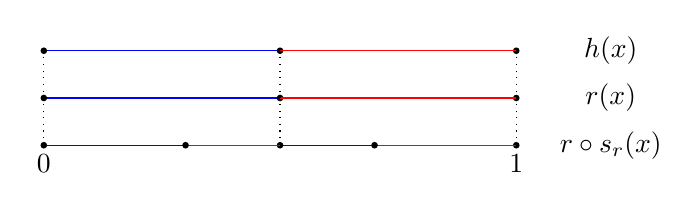
\begin{tikzpicture}[scale=0.6]
			% Blue horizontal line
			\draw[blue] (0,1) -- (5,1);
			\draw[blue] (0,0) -- (5,0);
			\draw[blue] (5,-1) -- (7,-1);
			\draw[blue] (0,-1) -- (3,-1);
			\fill[black] (5,0) circle (2pt);
			\fill[black] (0,0) circle (2pt);
			\fill[black] (10,0) circle (2pt);
			\fill[black] (5,1) circle (2pt);
			\fill[black] (0,1) circle (2pt);
			\fill[black] (10,1) circle (2pt);
			\fill[black] (0,-1) circle (2pt);
			\fill[black] (10,-1) circle (2pt);
			\fill[black] (5,-1) circle (2pt);
			\node[below] at (3,-1) {$\hminus$};
			\node[above] at (2.5,1) {$\minus$};
			\node[above] at (2.5,0) {$\minus$};
			\node[above] at (1.5,-1) {$\minus$};
			\node[above] at (6,-1) {$\minus$};

			% Red horizontal line
			\draw[red] (5,1) -- (10,1);
			\draw[red] (5,0) -- (10,0);
			\draw[red] (3,-1) -- (5,-1);
			\draw[red] (7,-1) -- (10,-1);
			\fill[black] (3,-1) circle (2pt);
			\fill[black] (7,-1) circle (2pt);
			\node[below] at (7,-1) {$\hplus$};
			\node[above] at (7.5,1) {$\plus$};
			\node[above] at (7.5,0) {$\plus$};
			\node[above] at (4,-1) {$\plus$};
			\node[above] at (8.5,-1) {$\plus$};

			\draw[black,dotted] (0,1) -- (0,-1);
			\draw[black,dotted] (5,1) -- (5,-1);
			\draw[black,dotted] (10,1) -- (10,-1);
			\node[below] at (0,-1) {$0$};
			\node[below] at (10,-1) {$1$};
			\node[below] at (5,-1) {$\h$};
			\node at (12,0) {$r(x)$};
			\node at (12,-1) {$r \circ s_r(x)$};
			\node at (12,1) {$h(x)$};
		\end{tikzpicture}
        \caption{Naive classifier.}
	\end{figure}
\end{exg}


In the next example, we calculate the error made by the deterministic Stackelberg equilibrium.
\begin{exg}	Let $r^*$ be a deterministic Stackelberg equilibrium obtained from Theorem \ref{thm:Deterministic Stackelberg equilibrium strategy}. Then $r^*$ is given by

	\begin{equation*}
		\begin{aligned}
			r^*(x) = \begin{cases}
				h(x) & \text{if } x \in [0,\hminus) \cup (\hplus,1]\\
				\Delta & \text{if } x \in [\hminus,\hplus],
			\end{cases}
		\end{aligned}
	\end{equation*}
	where $\hminus = \h - \uu$ and $\hplus = \h + \uu$. The sender's worst-case best response is
	\begin{equation*}
		\begin{aligned}
			s_{r^*}(x) = \begin{cases}
				x & \text{if } x \in [0,\hminus) \cup (\hplus,1]\\\
				\hplus & \text{if } x \in [\hminus,\h) \\
				\hminus & \text{if } x \in [\h,\hplus].
			\end{cases}
		\end{aligned}
	\end{equation*}
Hence $E(r^*) = [\hminus,\hplus]$ and $\cg{E}(r^*) = 2\uu$. This shows that ignoring feature vectors near the decision boundaries, which in any case will be misclassified under the naive decision rule, prevents other neighbouring feature vectors from getting misclassified.
	\begin{figure}
		\centering
		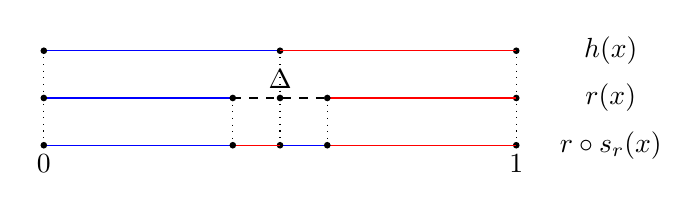
\begin{tikzpicture}[scale=0.6]
			% Blue horizontal line
			\draw[blue] (0,1) -- (5,1);
			\draw[blue] (0,0) -- (4,0);
			\draw[blue] (5,-1) -- (6,-1);
			\draw[blue] (0,-1) -- (4,-1);
			\fill[black] (5,0) circle (2pt);
			\fill[black] (0,0) circle (2pt);
			\fill[black] (10,0) circle (2pt);
			\fill[black] (5,1) circle (2pt);
			\fill[black] (0,1) circle (2pt);
			\fill[black] (10,1) circle (2pt);
			\fill[black] (0,-1) circle (2pt);
			\fill[black] (10,-1) circle (2pt);
			\fill[black] (5,-1) circle (2pt);
			\node[below] at (4,-1) {$\hminus$};
			\node[above] at (2.5,1) {$\minus$};
			\node[above] at (2.5,0) {$\minus$};
			\node[above] at (2,-1) {$\minus$};
			\node[above] at (5.5,-1) {$\minus$};

			% Red horizontal line
			\draw[red] (5,1) -- (10,1);
			\draw[red] (6,0) -- (10,0);
			\draw[red] (4,-1) -- (5,-1);
			\draw[red] (6,-1) -- (10,-1);
			\fill[black] (4,0) circle (2pt);
			\fill[black] (6,0) circle (2pt);
			\fill[black] (4,-1) circle (2pt);
			\fill[black] (6,-1) circle (2pt);
			\node[below] at (6,-1) {$\hplus$};
			\node[above] at (7.5,1) {$\plus$};
			\node[above] at (7.5,0) {$\plus$};
			\node[above] at (4.5,-1) {$\plus$};
			\node[above] at (8,-1) {$\plus$};
			\node[above] at (5,0) {$\Delta$};


			\draw[dashed] (4,0) -- (6,0);
			\draw[black,dotted] (0,1) -- (0,-1);
			\draw[black,dotted] (5,1) -- (5,-1);
			\draw[black,dotted] (10,1) -- (10,-1);
			\draw[black,dotted] (4,0) -- (4,-1);
			\draw[black,dotted] (6,0) -- (6,-1);
			\node[below] at (0,-1) {$0$};
			\node[below] at (10,-1) {$1$};
			\node[below] at (5,-1) {$\h$};
			\node at (12,0) {$r(x)$};
			\node at (12,-1) {$r \circ s_r(x)$};
			\node at (12,1) {$h(x)$};
		\end{tikzpicture}
        \caption{Deterministic Stackelberg equilibrium.}
	\end{figure}
\end{exg}

In Section \ref{subsec:Deterministic strategy}, we analyzed the setup where the sender adopts the worst-case best response. In contrast, Section \ref{subsec:Stochastic strategy} examined the setup where the sender employs the worst-case lazy best response. To ensure a fair comparison between the deterministic and stochastic Stackelberg equilibria, the sender's style of play should remain fixed. Therefore, in the following example, we calculate the classification error made by a receiver strategy, assuming the sender adopts the worst-case best response.


\begin{exg}\label{ex:eps stochastic strategy}
Let $\eps >0 $. Let $r_\eps \equiv (1-q_\eps(x),q_{\eps}(x),0)$ be stochastic receiver strategy where $q_\eps$ is defined as \begin{equation}\label{eqn:q eps formula}
		q_\eps(x) = \begin{cases}
			0 & \text{if } x \in [0,\hminuseps) \\
			\frac{x-\hminuseps}{2(\uu + \eps)}& \text{if } x \in [\hminuseps,\hpluseps]\\
		  1 & \text{if } x \in (\hpluseps,1],
		\end{cases}
	\end{equation}
where $\hminuseps := \h - \uu - \eps$ and $\hpluseps := \h + \uu + \eps$.
It follows that the worst-case best response is $s_{r_\eps}(x) = x$ (the calculation is similar to what is done in Lemma \ref{lem:error is half} and is given in Section~\ref{sec:proofs_ch2}, Calculation~\ref{cal:eps stochastic strategy}) and $\cg{E}(r_\eps)$ is $\frac{\uu + \eps}{2}$. This strategy shows that randomizing classifications near the decision boundaries can correctly classify feature vectors close to the decision boundaries, albeit with a low but positive probability. This happens because randomization ensures that the cost increase is offset by the increase in utility (which takes a fractional value due to randomization).
    \begin{figure}
		\centering
		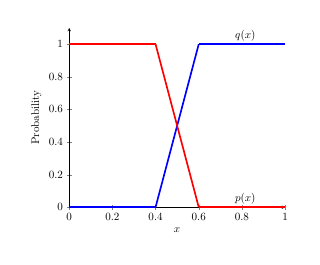
\begin{tikzpicture}[scale=0.4]
			\begin{axis}[
				axis lines = left,
				xlabel =$x$,
				ylabel = {Probability},
				xmin = 0,
				xmax = 1,
				ymin = 0,
				ymax = 1.1,
				legend pos = north west,
				]

				% Piecewise function q_{\eps}(x)
				\addplot[
				domain=0:0.4,
				samples=100,
				color=blue,
				line width=2.5pt,
				]{0};
				\addplot[
				domain=0.4:0.6,
				samples=100,
				color=blue,
				line width=1.5pt,
				]{5 * (x - 0.4)};
				\addplot[
				domain=0.6:1,
				samples=100,
				color=blue,
				line width=1.5pt,
				]{1};

				% Piecewise function p(x)
				\addplot[
				domain=0:0.4,
				samples=100,
				color=red,
				line width=1.5pt,
				]{1};
				\addplot[
				domain=0.4:0.6,
				samples=100,
				color=red,
				line width=1.5pt,
				]{-5*(x)+3};
				\addplot[
				domain=0.6:1,
				samples=100,
				color=red,
				line width=2.5pt,
				]{0};

				% Add labels
				\node[right] at (axis cs: 0.35,0.2) {};
				\node[right] at (axis cs: 0.5,0.7) {};
				\node[right] at (axis cs: 0.75,1.05) {$q_{\eps}(x)$};
				\node[right] at (axis cs: 0.75,-0.2) {};
				\node[right] at (axis cs: 0.5,-0.7) {};
				\node[right] at (axis cs: 0.75,0.05) {$p(x)$};

			\end{axis}
		\end{tikzpicture}
		\caption{Stochastic decision rule$r(x)$,$\uu = 0.1$,$\h = 0.5$}
		\label{fig:Stochasticdecisionrule}
	\end{figure}
\end{exg}

It can be seen from these examples that both the deterministic and stochastic Stackelberg equilibria outperform the naive classifier. Furthermore, the stochastic classifier makes fewer errors than the deterministic classifier. The benefit of randomization in strategic interactions is well-established in game theory literature, and we now observe its advantages in the strategic classification as well.

One crucial point to note is that although the penalty label was useful in the deterministic classifier, it was not helpful in the stochastic classifier. Furthermore, the deterministic classifier is sub-optimal compared to the stochastic classifier. Thus, the randomization offers the receiver a richer source of leverage to make the sender behave appropriately than the penalty label. However, in many cases, such as university admissions, for transparency, the receivers are constrained to use only the deterministic classifier. Thus, in those cases, the penalty label can act as compensation for the lack of randomization.

The following example describes the deterministic Stackelberg equilibrium of the university admission problem introduced in the Section \ref{sec:Introduction}.

\begin{exg}(Stackelberg equilibrium of the university admission problem):\\

Recall the example from the introduction. Suppose a university offers two programs: Theoretical Physics and Experimental Physics. Admission to these programs is determined by each student’s performance on an entrance exam. Each prospective student has a unique combination of theoretical and experimental skills, and their \textit{true program} corresponds to the program that aligns with their stronger skill. However, students often prefer a program that does not align with their true program. The university’s goal is to design the entrance exam to maximize the number of students admitted to their true program.

We model this as a strategic classification problem as follows: The university acts as the receiver, and the student as the sender. Let $\cg{X} := [0,1]$ represent the set of feature vectors, where $x \in \cg{X}$ denotes a student's true aptitude, with the interpretation that it has $x$ theoretical skill and $(1 - x)$ experimental skill. We assume that true aptitudes are uniformly distributed across the student population; thus, $D$, the probability law on $\cg{X}$, is uniform. Let $\cg{Y} := \{\minus,\plus\}$ denote the label space, where $\minus$ indicates the Experimental Physics program and $\plus$ the Theoretical Physics program. The true function $h(x)$, which assigns each student to their true program, is given by the following equation:
\begin{equation}
    h(x) = \begin{cases}
    \plus & \text{if } x > 0.5, \\
    \minus & \text{if } x \leq 0.5.
    \end{cases}
\end{equation}
This means $\h = 0.5$, and that for $x > 0.5$, a student’s true program is Theoretical Physics, while for $x \leq 0.5$, it is Experimental Physics.

The university has access to a question bank containing questions of varying difficulties. We denote the difficulty level of a question by $x$, indicating that the question requires $x$ theoretical knowledge and $(1 - x)$ experimental knowledge to solve. Note that there is a one-to-one correspondence between the feature vector set $\cg{X}$ and the question bank. Thus, a student may demonstrate an aptitude $x'$ (not necessarily their true aptitude) by solving a question with difficulty level $x'$. The entrance exam comprises multiple questions selected from this bank, with each question associated with a program. A student can attempt only one question, and admission to the corresponding program is granted if they answer correctly.

We assume each student's preferred program differs from their true program. The student’s utility function is given by
\begin{equation}
	U(y,x) := \begin{cases}
		0.04 & x \in [0,0.5], y = \plus \\
		0.04 & x \in (0.5,1], y = \minus \\
		0 & y = h(x)\\
		-\infty & y = \Delta.
	\end{cases}
\end{equation}
This means $\um = \up = 0.04$ , and a student gains a utility of $0.04$ if assigned to their preferred program and $0$ if assigned to their true program and $-\infty$ if not assigned any program. The cost kernel is given by $\phi(x) = x$, meaning that for a question with difficulty level $x'$, a student with true aptitude $x$ incurs a cost of $|x - x'|$ while solving it.

The university's strategy set includes all possible question papers for the entrance exam. For a given question paper, each student selects the question that maximizes their utility at the lowest cost, potentially demonstrating an aptitude $x'$ different from their true aptitude to the university. The student’s strategy set consists of mappings that specify which question to attempt for each question paper. We assume students answer their chosen question correctly. Consequently, the university, aware of students' strategic behaviour, must optimally design the question paper to maximize the number of students admitted to their true program.

According to Theorem \ref{thm:Deterministic Stackelberg equilibrium strategy}, questions with difficulty levels in the interval $[\h- \um,\h+\up]$ should not be included in the exam. Substituting the value for  $\h,\um,\up$ for this example, this interval turns out to be $[0.48,0.52]$. Furthermore, the students who correctly answers questions with difficulty levels less than $0.48$ should be admitted to the Experimental Physics program, and the students who correctly answers the questions with difficulty levels greater than $0.52$ should be admitted to the Theoretical Physics program. The intuition for excluding questions in the interval $[0.48,0.52]$ is as follows: if a question of difficulty level, say $0.51$ (corresponding to Theoretical Physics) is included, a student with true aptitude $0.49$ (whose true program is Experimental Physics) could solve it with only effort $0.02$, leading to misclassification. However, this approach has a drawback: students whose true aptitudes lie within the interval $[0.48,0.52]$ must attempt questions of difficulty level outside this range. Thus, by incurring a cost, they attempt questions linked to their preferred program and get misclassified by the university. Nonetheless, the overall benefits of this strategy outweigh its drawbacks, making it the optimal option for the university.

\end{exg}


\subsection{Other Stackelberg equilibria}\label{subsec:Other equilibria}
In this section, we only consider deterministic Stackelberg equilibria. In many scenarios, the strategic classification problem may admit more than one Stackelberg equilibrium. While all such Stackelberg equilibria guarantee the same classification error for the receiver, they are not equivalent from the sender's perspective. Here, we discuss various considerations that a receiver may take into account besides minimizing the classification error.

\subsubsection{Participation constraint for the sender}
Consider the following instance of the problem. Let $D$ be a uniform distribution on $\cg{X}$, with $\h = 0.5$ and $\um = \up = 0.1$. It can be shown that both $r_1$ and $r_2$, defined as
\begin{equation*}
r_1(x) = \begin{cases}
\minus & \text{if } x \in [0, 0.45] \\
\Delta & \text{if } x \in (0.45, 0.55) \\
\plus & \text{if } x \in [0.55, 1]
\end{cases}, \;\;\;\;
r_2(x) = \begin{cases}
\minus & \text{if } x = 0 \\
\Delta & \text{if } x \in (0, 1) \\
\plus & \text{if } x = 1
\end{cases}
\end{equation*}
are receiver Stackelberg equilibrium strategies. However, the situation differs from the sender's perspective. For $x \in \cg{X}$, the sender's payoff under $r_1$ and $r_2$ satisfies
\begin{equation}
\mathbb{U}(x; r_1, s_{r_1}) \geq \mathbb{U}(x; r_2, s_{r_2}) \text{ for all } x \in \cg{X}.
\end{equation}
That is, for each $x \in \cg{X}$, the payoff for the sender under $r_1$ is greater than or equal to that under $r_2$.

This scenario resembles a dilemma in the principal-agent problem, where the principal can impose an unfair contract on the agent, who ends up paying (instead of being paid) for their work. To remedy this in the principal-agent context, the agent is given the option to refuse the contract and receive a baseline payoff. This encourages the principal to offer a contract with a payoff greater than the baseline. This concept is known as the \textit{participation constraint} for the agent.

Drawing a parallel to the principal-agent problem, the receiver can be viewed as the principal who offers a contract $r$, while the sender acts as the agent who, by making effort $s$ on a feature vector $x$, gets a payoff of $\mathbb{U}(x; r, s)$. We allow the sender, after seeing the contract $r$, the option not to participate and instead receive a baseline payoff. There are many ways the sender can determine his decision to participate. Here, we assume that the sender does not participate if $\mathbb{U}(x; r, s_r)$ is lower than the baseline payoff for any $x \in \cg{X}$. We further assume that if the sender does not participate in the game, the receiver makes an error on the entire $\cg{X}$. This participation constraint of the sender would discourage the receiver from playing a degenerate strategy like $r_2$, since the sender would reject such a game. Given this constraint, strategies like $r_1$, with a $\Delta$ interval of length $\uu$, provide justifiable non-degenerate Stackelberg equilibria, as we show in the following cases.


\noindent \textit{Case 1 (Negative participation constraint): }\\
Suppose the sender incurs a fixed payoff $\nu \leq 0$ if it chooses not to participate in the game after seeing the receiver's strategy. This means the sender can opt-out with a small penalty upon encountering an unfavourable receiver strategy. Consequently, many degenerate receiver strategies like $r_2$ will not satisfy the participation constraint and will no longer be a receiver Stackelberg equilibrium.

Now consider the strategy $r_1$. For $x \in [0, 0.45) \cup (0.55, 1]$, the sender's payoff at $x$ is $\mathbb{U}(x; r, s_r) = 0$. For $x \in [0.45, 0.5]$, the sender's payoff at $x$ is $\mathbb{U}(x; r, s_r) = x - 0.45$ and for $x \in (0.55, 1]$, the sender's payoff at $x$ is $\mathbb{U}(x; r, s_r) = 0.55 - x$. Thus, $\min_{x \in \cg{X}} \mathbb{U}(x; r, s_r) = 0$. This satisfies the sender's participation constraint, and hence the sender will participate in the game. Therefore, $r_1$ is a Stackelberg equilibrium even under this constraint.

\noindent \textit{Case 2 (Positive participation constraint): }\\
Suppose the sender receives a fixed payoff $\nu > 0$ if it chooses not to participate in the game after seeing the receiver's strategy. We will show that every receiver strategy is a Stackelberg equilibrium strategy.

Let $r$ be a receiver strategy. If $E(r, s_r, h) = \cg{X}$, then $\cg{E}(r) = 1$. If $E(r, s_r, h) \neq \cg{X}$, then there exists $x$ such that $r(s_r(x)) = h(x)$. This implies $\mathbb{U}(x; r, s_r) = -|s_r(x) - x| \leq 0$. But this violates the sender's participation constraint, and thus the sender will ignore this strategy $r$. Therefore, $\cg{E}(r) = 1$. Hence, $\cg{E}(r) = 1$ for all $r \in \msf{R}$. Therefore, every receiver strategy $r \in \msf{R}$ is a receiver Stackelberg equilibrium strategy as claimed. More specifically, $r_1$ is a Stackelberg equilibrium even under this constraint.


\subsubsection{Fairness and complexity of the classifier:}
Let $D$ be the uniform probability law on $[0,1]$, $\h = 0.5$, and $\um = \up = 0.1$. From Theorem \ref{thm:Deterministic Stackelberg equilibrium strategy}, any strategy $r(x; \hminus, \hplus) \in \sr{R}$ such that $\hminus \leq 0.5 \leq \hplus$ and $|\hminus - \hplus| = 0.1$ is a Stackelberg equilibrium. These equilibria yield the same receiver error but differ in how errors are distributed across each label class.

Consider two such receiver strategies, $r_1$ and $r_2$, with 
corresponding $\Delta$-regions $(0.45, 0.55)$ and $(0.4, 0.5)$, 
respectively. The strategy $r_1$ appears fairer, as it balances 
the ratio of correctly classified labels, compared to $r_2$, 
which misclassifies only the $-$ class. However, the receiver 
strategy $r_2$ is simpler, with 2 decision boundaries in 
$r_2 \circ s_{r_2}$ compared to 3 in $r_1 \circ s_{r_1}$. 
This simplicity is an advantage for learnability; 
the VC dimension of a hypothesis class increases with the number of decision 
boundaries that functions in that class are allowed to have
(see Proposition \ref{prop: VC dimension}). This 
highlights a trade-off between fairness and 
efficient learnability. Depending on the 
application, one strategy may be preferable to the other.

\begin{figure}
		\centering
		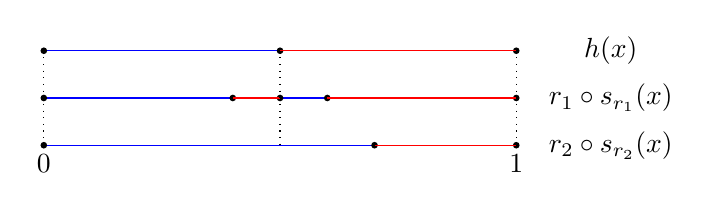
\begin{tikzpicture}[scale=0.6]
			% Blue horizontal line
			\draw[blue] (0,1) -- (5,1);
			\draw[blue] (0,0) -- (4,0);

                \draw[blue] (5,0) -- (6,0);
			\draw[blue] (0,-1) -- (7,-1);
			\fill[black] (4,0) circle (2pt);
                \fill[black] (6,0) circle (2pt);
                \fill[black] (5,0) circle (2pt);
			\fill[black] (0,0) circle (2pt);
			\fill[black] (10,0) circle (2pt);
			\fill[black] (5,1) circle (2pt);
			\fill[black] (0,1) circle (2pt);
			\fill[black] (10,1) circle (2pt);
			\fill[black] (0,-1) circle (2pt);
			\fill[black] (10,-1) circle (2pt);
			\fill[black] (7,-1) circle (2pt);

			\node[above] at (2.5,1) {$\minus$};
			\node[above] at (2.5,0) {$\minus$};
			\node[above] at (3.5,-1) {$\minus$};
                \node[above] at (5.5,0) {$\minus$};


			% Red horizontal line
			\draw[red] (5,1) -- (10,1);
			\draw[red] (6,0) -- (10,0);
                \draw[red] (4,0) -- (5,0);

			\draw[red] (7,-1) -- (10,-1);

			\node[above] at (7.5,1) {$\plus$};
                \node[above] at (4.5,0) {$\plus$};

			\node[above] at (7.5,0) {$\plus$};

			\node[above] at (8.5,-1) {$\plus$};
			%\node[above] at (5,0) {$\Delta$};



			\draw[black,dotted] (0,1) -- (0,-1);
			\draw[black,dotted] (5,1) -- (5,-1);
			\draw[black,dotted] (10,1) -- (10,-1);
			\node[below] at (0,-1) {$0$};
			\node[below] at (10,-1) {$1$};
			\node[below] at (5,-1) {$\h$};
			\node at (12,0) {$r_1 \circ s_{r_1}(x)$};
			\node at (12,-1) {$r_2 \circ s_{r_2}(x)$};
			\node at (12,1) {$h(x)$};
		\end{tikzpicture}
        \caption{Fairness and complexity tradeoff.}
	\end{figure}


\section{Learning the Stackelberg equilibrium}\label{sec:Learning problem}
In this section, we address the learning problem, where the receiver is unaware of the true function and is limited to employing only deterministic strategies. Let $\cg{F} \subseteq \{f \mid f:\cg{X} \rightarrow \cg{Y}\}$  denote a hypothesis class, and let  $$ l(x,y; f) := \mathbbm{1}_{f(x) \neq y} $$
be the \textit{zero-one loss function}, where $x \in \cg{X}, y \in \cg{Y}$ and $f \in \cg{F}$.
Let $(X,Y)$ be a random variable over $(\cg{X},\cg{Y})$ and $D$ be its corresponding probability law.
Let $L_{D}(f)$ denote the \textit{risk function} corresponding to the zero-one loss function and be defined as 
\begin{equation}\label{eqn:risk function}
    L_D(f) :=
    \E_{D}[l(X,Y;f)].
\end{equation}
Suppose $Y = h(X)$, where $h$ is the true function. Then we modify the definition of risk function given in \eqref{eqn:risk function}.
Let $X$ random variable over $\cg{X}$ and $D$ be it corresponding probability law. Then $L_D(f;h)$ denotes the \textit{$h$-risk function} corresponding to the zero-one loss function and be defined as 
\begin{equation}
    L_D(f;h) :=   \E_{D}[l(X,h(X);f)].
\end{equation}
In the absence of strategic interactions between the sender and the receiver, a hypothesis class is PAC (Probably Approximately Correct) learnable if it satisfies the following definition (which is the same as Definition 3.1 in \cite{shalev-shwartz_ben-david_2014}).

\begin{defn}\label{def:PAC learning}\index{PAC learning|textbf}
A hypothesis class $\cg{F}$ is PAC learnable if there exists a function $m_{\cg{F}}^{\mathrm{PAC}}: (0,1)^2 \to \N$ and a learning algorithm $A: \cup_{n=1}^\infty (\cg{X} \times \cg{Y})^n \to \cg{F}$ such that for every $(\eps, \dlt) \in (0,1)^2$, for every true function $h \in \cg{F}$ and every probability law $D$ over $\cg{X}$, the following holds:
Let $S = \{(x_i, h(x_i))\}_{i=1}^m$ be a sample where $x_i$'s are drawn i.i.d. from  $D$ and $m \geq m_{\cg{F}}^{\mathrm{PAC}}(\eps,\dlt)$. Then
\[
D^{\otimes m}\left( L_{D}(A(S);h)  < \eps \right) > 1 - \dlt.
\]
\end{defn}
There exists a more general notion of PAC learning called agnostic PAC learning which is defined in the following definition (which is the same as Definition 3.3 in \cite{shalev-shwartz_ben-david_2014}).
\begin{defn}\label{def:agnostic PAC learning}\index{Agnostic PAC learning|textbf}\index{PAC learning!agnostic|textbf}
A hypothesis class $\cg{F}$ is agnostic PAC learnable if there exists a function $m_{\cg{F}}^{\mathrm{agn}}: (0,1)^2 \to \N$ and a learning algorithm $A: \cup_{n=1}^\infty (\cg{X} \times \cg{Y})^n \to \cg{F}$ such that for every $(\eps, \dlt) \in (0,1)^2$ and every probability law $D$ over $\cg{X} \times \cg{Y}$, the following holds: Let $S = \{(x_i, y_i)\}_{i=1}^m$ be a sample where 
$(x_i, y_i)$'s are drawn i.i.d. from  $D$ and 
$m \geq m_{\cg{F}}^{\mathrm{agn}}(\eps, \dlt)$. Then
\[
D^{\otimes m}\left( L_{D}(A(S)) - \inf_{f \in \cg{F}} L_{D}(f) < \eps \right) > 1 - \dlt.
\]
\end{defn}
An algorithm $A$ is a \textit{successful PAC/agnostic PAC learner} of $\cg{F}$ if $\cg{F}$ is PAC/agnostic PAC learnable and $A$ is the corresponding learning algorithm defined in Definition \ref{def:PAC learning}/\ref{def:agnostic PAC learning}. Consider the learning algorithm Empirical risk minimization (ERM) 
\[\text{ERM}:\cup_{n=1}^\infty(\cg{X}\times \cg{Y})^n \rightarrow \cg{F} \text{ defined as } 
\text{ERM}(\{(x_i, y_i)_{i=1}^m\}) := \arg\min_{f \in \cg{F}} \frac{1}{m} \sum_{i=1}^m l(x_i, y_i; f).
\]
A hypothesis class $\cg{F}$ is said to have the \textit{uniform convergence property} if there exists a function $m_{\cg{F}}^{\mathrm{UC}}: (0,1)^2 \to \N$ such that for every $(\eps, \dlt) \in (0,1)^2$ and every probability law $D$ over $\cg{X} \times \cg{Y}$, if $S = \{(x_i, y_i)\}_{i=1}^m$ is a sample drawn i.i.d. from $D$ with $m \geq m_{\cg{F}}^{\mathrm{UC}}(\eps, \dlt)$, then
\[
D^{\otimes m}\left( \sup_{f \in \cg{F}} \left| \frac{1}{m} \sum_{i=1}^m l(x_i, y_i; f) - L_D(f) \right| < \eps \right) > 1 - \dlt.
\]
The following theorem shows that uniform convergence, PAC learnability, agnostic PAC learnability, and the success of ERM rules are all characterized by the finiteness of the VC dimension.

\begin{thm}[Fundamental theorem of statistical learning]\label{thm:Fundamental theorem of statistical learning}\index{Fundamental Theorem of Statistical Learning|textbf}\index{VC dimension|textbf}
Let  $\cg{F} \subseteq \{f \mid f:\cg{X} \rightarrow \cg{Y}\}$ be a hypothesis class of functions from domain $\cg{X}$ to $\cg{Y} = \{0,1\}$ and let the loss function be the $0-1$ loss. Then, the following statements are equivalent:

\begin{enumerate}[label=\alph*)]
    \item $\cg{F}$ has the uniform convergence property.
    \item Any ERM rule is a successful agnostic PAC learner for $\cg{F}$.
    \item $\cg{F}$ is agnostic PAC learnable.
    \item $\cg{F}$ is PAC learnable.
    \item Any ERM rule is a successful PAC learner for $\cg{F}$.
    \item $\cg{F}$ has finite VC dimension ($\text{VC dim}(\cg{F}) < \infty$).
\end{enumerate}
Furthermore, if $\text{VC dim}(\cg{F}) = d < \infty$, there exist absolute constants $C_1, C_2 > 0$ such that for any $(\eps,\dlt) \in (0,1)^2$, the sample complexities satisfy:
\begin{enumerate}[1.]
    \item $\cg{F}$ has the uniform convergence property with sample complexity
    \begin{equation}\label{eqn:sample complexity:UC}
    C_1\frac{d + \log\left(\frac{1}{\dlt}\right)}{\eps^2} \leq m_{\cg{F}}^{\mathrm{UC}}(\eps,\dlt) \leq C_2\frac{d + \log\left(\frac{1}{\dlt}\right)}{\eps^2},
    \end{equation}
    \item $\cg{F}$ is agnostic PAC learnable with sample complexity
    \begin{equation}\label{eqn:sample complexity:thm:Fundamental theorem of statistical learning}
    C_1\frac{d + \log\left(\frac{1}{\dlt}\right)}{\eps^2} \leq m_{\cg{F}}^{\mathrm{agn}}(\eps,\dlt) \leq C_2\frac{d + \log\left(\frac{1}{\dlt}\right)}{\eps^2},
    \end{equation}
    \item $\cg{F}$ is PAC learnable with sample complexity
    \begin{equation}\label{eqn:sample complexity:PAC}
    C_1\frac{d + \log\left(\frac{1}{\dlt}\right)}{\eps} \leq m_{\cg{F}}^{\mathrm{PAC}}(\eps,\dlt) \leq C_2\frac{d \log\left(\frac{1}{\eps}\right) + \log\left(\frac{1}{\dlt}\right)}{\eps}.
    \end{equation}
\end{enumerate}
\end{thm}

\begin{proof}
Refer to Theorems 6.7 and 6.8 in \cite{shalev-shwartz_ben-david_2014}.
\end{proof}

We now establish a similar learning criterion for a hypothesis class $\cg{F}$ in the context of strategic classification. Recall that for a true function $f \in \cg{F}$ and probability law $D \in \fk{D}$, $r^\star_{f,D}$ denotes the Stackelberg equilibrium as defined in Definition \ref{def:Stackelberg equilibrium}. Define $\widetilde{\cg{F}} := \{r^\star_{f,D} \circ s_{r^\star_{f,D}} : f \in \cg{F}, D \in \fk{D}\}$, referred to as the \emph{Stackelberg hypothesis class}, which represents the space of receiver Stackelberg equilibria derived from $\cg{F}$ and $\fk{D}$. A hypothesis class $\cg{F}$ is strategically learnable if it satisfies the following definition.

\begin{defn}[Strategically learnable class]\label{def:Strategically learnable class}\index{Strategically learnable class|textbf}\index{Strategic learnability|textbf}
A hypothesis class $\cg{F}$ is strategically learnable if there exists a function $m_{\cg{F}}: (0,1)^2 \to \N$ and a learning algorithm $A: \cup_{n=1}^\infty (\cg{X} \times \cg{Y})^n \to \widetilde{\cg{F}}$ such that for any true function $h \in \cg{F}$, any probability law $D \in \fk{D}$, and any $(\eps, \dlt) \in (0,1)^2$, the following holds: Let $S = \{(x_i, h(x_i))_{i=1}^m\}$ be a sample where $x_i$ are drawn i.i.d. from $D$ and $m \geq m_{\cg{F}}(\eps, \dlt),$
then
\begin{equation}\label{def: strategically learnable}
D^{\otimes m}\Big( \cg{E}(A(S); h, D) - \cg{E}(r^\star_{h, D}; h, D) < \eps \Big) > 1 - \dlt.
\end{equation}
The function $m_{\cg{F}}(\eps, \dlt)$ is called the sample complexity of the algorithm.
\end{defn}


Our definition of strategic learnability is different from \cite{sundaram2021pac} because we let the algorithm search over the Stackelberg equilibrium hypothesis class (i.e., over $r_f, f \in \mathcal{F}$) rather than the original hypothesis class (i.e., over $f \in \mathcal{F}$). 


We propose two algorithms for learning a strategic classifier: \textit{vanilla ERM} and \textit{strategy aware ERM} (defined in Section \ref{subsec:Vanilla ERM} and \ref{subsec:Stragically aware ERM} respectively). We show that a hypothesis class is strategically learnable if and only if it is learnable under the strategy-aware ERM algorithm. 
However, there exist strategically learnable hypothesis classes which are not
learnable under the vanilla ERM algorithm.

Assuming the hypothesis class is learnable by each algorithm, we compare their ease of learning (compared in Section \ref{subsec:comparision}). This is controlled by the VC dimension of the hypothesis class, which determines the sample complexity in PAC learning. We observe that when the hypothesis class is complex (i.e., contains functions with many decision boundaries), strategy-aware ERM makes learning easier, as it can reduce the VC dimension of the effective learning space. Conversely, for simpler hypothesis classes, vanilla ERM is often the the more direct and efficient approach.


\subsection{Some results on hypothesis class with multiple decision boundaries}

A point is called a \textit{decision boundary}, if it assigns different labels to its left and right neighbours. 
The hypothesis class we consider for our learning algorithms comprises of functions with multiple decision boundaries, requiring us to extend the results established in Theorem \ref{thm:Deterministic Stackelberg equilibrium strategy} (which only had one decision boundary). To achieve this, we examine a generalized version of a decision problem where the true function has multiple decision boundaries. Let $\cg{X} = [0,1]$ represent the feature vector space, and let $\cg{Y} = \{-1, +1\}$ be the label space, and $D \in \fk{D}$ a probability law on $\cg{X}$. Decompose $\cg{X} \text{ as } \cg{X} = O_1 \cup O_2 \cup \cdots \cup O_{d-1}$, where each $O_n$ is a disjoint interval defined as $O_n = [o_{(n)}, o^{(n)})$ for $n < d-1$, $O_{d-1} = [o_{d-1}, 1]$, and $o^{(n)} = o_{(n+1)}$. Define the true function $h(x)$ as follows:
\begin{equation}\label{eqn:multiple boundary true function}
    h(x) = \begin{cases}
        \minus & \text{if } x \in O_n, \; n \text{ is even}, \\
        \plus & \text{if } x \in O_n, \; n \text{ is odd}.
    \end{cases}
\end{equation}
Let the cost kernel be $\phi(x) = x$, and let $\Delta$ denote the penalty label (as considered in Section \ref{sec:Problem formulation}). Define the utility function $U(y,x)$ as:
\begin{equation}\label{eqn:Utility2}
    U(y,x) := \begin{cases}
        \uu & \text{if } x \in O_n, \; y = \plus, \; n \text{ is even}, \\
        \uu & \text{if } x \in O_n, \; y = \minus, \; n \text{ is odd}, \\
        0 & \text{if } y = h(x), \\
        -\infty & \text{if } y = \Delta.
    \end{cases}
\end{equation}
The structure of the Stackelberg equilibrium strategy generalizes Theorem \ref{thm:Deterministic Stackelberg equilibrium strategy} (when $\up = \um$) and is stated in the following proposition.

\begin{prop}\label{prop:Deterministic Stackelberg equilibrium for multiple decision boundaries}
	Let $D$ be a probability law on $\cg{X}$, and let $h(x)$ be the true function. Suppose a Stackelberg equilibrium exists for the receiver. Then there exist intervals $\Theta_n \subseteq O_n$ for $n \in \{1, \dots, d-1\}$, such that the receiver strategy $r$ defined by
	\begin{equation}\label{eqn:stack multiple}
		r(x;\Theta_1,\cdots,\Theta_{d-1}) = \begin{cases}
			h(x) & \text{if } x \in \cup_{n=1}^{d-1} \Theta_n, \\
			\Delta & \text{if } x \not\in \cup_{n=1}^{d-1} \Theta_n,
		\end{cases}
	\end{equation}
	is a Stackelberg equilibrium, and $r \circ s_r$ is of the form
	\begin{equation*}
		r(s_r(x)) = \begin{cases}
			h(x) & \text{if } x \in \cup_{n=1}^{d-1} \Theta_n, \\
			-h(x) & \text{if } x \not\in \cup_{n=1}^{d-1} \Theta_n.
		\end{cases}
	\end{equation*}
\end{prop}


\begin{proof} The proof of the proposition is given in Section~\ref{sec:proofs_ch2} (Proof~\ref{proof:Deterministic Stackelberg equilibrium for multiple decision boundaries}).
\end{proof}

Our next theorem establishes the VC dimension of a hypothesis class containing hypotheses with multiple decision boundaries.

\begin{prop}\label{prop: VC dimension}
    Let the hypothesis class $\mathcal{F} \subset \{f| f:\cg{X} \rightarrow \cg{Y}\}$ be a collection of all functions with at most $d-1$ decision boundaries. Then VC dim$(\mathcal{F}) = d$.
\end{prop}

\begin{proof} The proof of the proposition is given in Section~\ref{sec:proofs_ch2} (Proof~\ref{proof:VC_dimension}).
\end{proof}


\subsection{Vanilla ERM}\label{subsec:Vanilla ERM}
One intuitive algorithm for the receiver to learn the strategic classifier is to estimate the true function from the sample data. The receiver then plays the screening game under this estimated function, treating it as the true function, and outputs the corresponding Stackelberg equilibrium. The vanilla ERM algorithm expresses this idea.
Let $D \in \fk{D}$ be a probability law on $\cg{X}$, $h$ be the true function and let $S = \{(x_i, h(x_i))_{i=1}^m\}$ be a sample where $x_i$ are drawn i.i.d. from $D$. Let $D(S)$ be the empirical law of sample $S$ defined as:
\begin{equation}\label{eqn:empirical measure}
D(S)(B) := \frac{1}{m}\sum_{i=1}^m \mathbbm{1}_{x_i \in B}  
\end{equation}
where $B$ is a Borel measurable set in $\cg{X}$. 

\begin{center}
	\begin{algorithm2e}[H]\label{algo:Vanilla ERM}\index{Vanilla ERM algorithm|textbf}\index{Empirical Risk Minimization!vanilla ERM|textbf}
		\SetAlgoLined
		\DontPrintSemicolon
		\KwData{$\text{Hypothesis class }\cg{F}, \text{ Sample } S = \{(x_i,h(x_i))\}_{i=1}^m$,\\ $\text{Zero-one loss function } l_h(f,x) := \mathbbm{1}_{\{f(x) \neq h(x)\}}$}
		
		\KwResult{Hypothesis $\hat{r}_{erm}$}
		\BlankLine
		\tcp{Estimation}
		$A(S) := \arg\min_{f \in \cg{F}} \sum_{i=1}^m \mathbbm{1}_{\{f(x_i) \neq h(x_i)\}}$\\
		$D(S) :=\text{Empirical law }$ \\
		\BlankLine
		\tcp{Decision}
		$\hat{r} := r^\star_{A(S),D(S)}$, i.e., Stackelberg equilibrium under true function $\hat{h}$ and probability law $D(S)$\;
		\caption{Vanilla ERM algorithm}
	\end{algorithm2e}
\end{center}

The Algorithm \ref{algo:Vanilla ERM} is initialized by providing a hypothesis class $\cg{F}$ and a sample $S$. In the first step, the algorithm calculates $A(S)$, which estimates the true function $h$ from the sample $S$ via the ERM subroutine. In the second step, it calculates the empirical law $D(S)$ of sample $S$, which is an estimate of the input law $D$ on $\cg{X}$ from which the $x_i$'s in $S$ were chosen. In the third step, it calculates the Stackelberg equilibrium $r^\star_{A(S),D(S)}$ (refer Definition \ref{def:Stackelberg equilibrium}) under the (estimated) true function $A(S)$ and the probability law $D(S)$ on $\cg{X}$, as given in Theorem \ref{thm:Deterministic Stackelberg equilibrium strategy}. 

We show that if the hypothesis class $\cg{F}$ has finite VC dimension, then it is strategically learnable under the Algorithm \ref{algo:Vanilla ERM}.

\begin{thm}\label{thm:Startegic learning for vanilla ERM}
Let $\mathcal{F} \subseteq \{ f \mid f: \cg{X} \rightarrow \cg{Y} \}$ be a hypothesis class consisting of all functions with at most $d-1$ decision boundaries, where $d <\infty$. Let $A: \cup_{n=1}^\infty (\cg{X} \times \cg{Y})^n \rightarrow \mathcal{F}$ denote the Algorithm \ref{algo:Vanilla ERM} (vanilla ERM algorithm) and let $B: \cg{F} \rightarrow \widetilde{\cg{F}}$ map a hypothesis to its corresponding Stackelberg equilibrium. Then $\cg{F}$ is strategically learnable (cf. Definition \ref{def:Strategically learnable class}) under $B \circ A$.
\end{thm}

\begin{proof} The proof is given in Section~\ref{sec:proofs_ch2} (Proof~\ref{proof:strategic_learning_vanilla_erm}).
\end{proof}

We prove the theorem with the help of the following two lemmas. The first lemma states that for a fixed true function $f \in \cg{F}$, the classification errors of the Stackelberg equilibrium strategies $r^\star_{f,D}$ and $r^\star_{f,D(S)}$ are similar for all $D \in \fk{D}$.

\begin{lem}\label{lem:same true function}\index{Dvoretzky--Kiefer--Wolfowitz (DKW) inequality|textbf}
Let $(\eps, \dlt) \in (0,1)^2$. Let $f \in \cg{F}$ be a true function with at most $K$ true-label intervals (i.e., at most $K-1$ decision boundaries), and let $D \in \fk{D}$ be a probability law on $\cg{X}$. Let $S = \{(x_i, h(x_i))\}_{i=1}^m$ be a sample of size $m$, where the $x_i$'s are drawn i.i.d. according to a probability law $D$, and let $D(S)$ be the empirical law of the sample $S$. Let $r^{\star}_{D(S)}$ and $r^{\star}_{D}$ be the Stackelberg equilibrium under the true function $f$ for probability law $D(S)$ and $D$ respectively. Then, there exists an $\bar{m}(\eps,\dlt)$ such that for all $m > \bar{m}(\eps,\dlt)$ the following holds:
    \begin{equation*}
        D^{\otimes m}\big(\cg{E}(r^\star_{f,D(S)};f, D) - \cg{E}(r^\star_{f,D};f, D) \le 4K\eps\big) > 1 - 2e^{-2m\eps^2}.
    \end{equation*}
\end{lem}

\begin{proof} The proof is given in Section~\ref{sec:proofs_ch2} (Proof~\ref{proof:same true function}).
\end{proof}

The next lemma states that for a fixed probability law $D \in \fk{D}$, the classification errors of the Stackelberg equilibrium strategies $r^\star_{A(S),D}$ and $r^\star_{h,D}$ are similar. 
\begin{rem}
Notice that $r_{A(S),D}$ is the Stackelberg equilibrium when the estimated true function $A(S)$ is considered the true function. To avoid confusion with the actual true function $h$, which generated the samples, we will refer to $h$ as the \textit{ground true function} and $A(S)$ as the \textit{estimated true function} whenever there is potential for ambiguity.
\end{rem}

\begin{lem}\label{lem:same distribution}
Let $(\eps, \dlt) \in (0,1)^2$.
Let $\mathcal{F} \subseteq \{ f \mid f: \cg{X} \rightarrow \cg{Y} \}$ be a hypothesis class consisting of all functions with at most $d-1$ decision boundaries. Let $A: \cup_{n=1}^\infty (\cg{X} \times \cg{Y})^n \rightarrow \mathcal{F}$ denote the algorithm described in Algorithm \ref{algo:Vanilla ERM} (vanilla ERM algorithm).
For every ground true function $h \in \mathcal{F}$ and every probability law $D \in \fk{D}$ on $\cg{X}$, the following holds. Let $S = \{(x_i, h(x_i))\}_{i=1}^m$ be a sample of size $m$, where $x_i$ are drawn i.i.d. according to $D$. Let $r^\star_{A(S),D}$ and $r^\star_{h,D}$ be the Stackelberg equilibria under $D$ and the estimated true function $A(S)$ and the ground true function $h(x)$, respectively. Then there exists $\underline{m}(\eps,\dlt) := m_{\cg{F}}^{\mathrm{PAC}}(\eps,\dlt)$ such that for all $m \geq \underline{m}(\eps,\dlt)$, the following holds.

\begin{enumerate}[label=(\alph*)]
    \item \label{lem:same distribution (a)} The following inequality holds uniformly over all receiver strategies $r \in \msf{R}$:
    \begin{equation*}
        D^{\otimes m}\left(\sup_{r \in \msf{R}} |\mathcal{E}(r; h,D) - \mathcal{E}(r; A(S), D)| < \eps\right) > 1 - \dlt.
    \end{equation*}

    \item \label{lem:same distribution (b)} For receiver Stackelberg equilibria $r^\star_{A(S),D}$ and $r^\star_{h,D}$, we have \begin{equation}\label{eqn:lem:vanilla ERM PAC bound}
    D^{\otimes m}\big(\mathcal{E}(r^\star_{A(S),D}; h,D) - \mathcal{E}(r^\star_{h,D}; h, D) < 2\eps\big) > 1 - \dlt.
\end{equation}

Furthermore, the sample complexity $\underline{m}(\eps,\dlt)$ satisfies
\begin{equation}\label{eqn:sample complexity:lem:same distribution}
    \begin{aligned}
        C_1 \frac{d + \log\left(\frac{1}{\dlt}\right)}{\eps} &\leq \underline{m}(\eps,\dlt) \leq C_2 \frac{d \log\left(\frac{1}{\eps}\right) + \log\left(\frac{1}{\dlt}\right)}{\eps}
    \end{aligned}.
\end{equation}
Here $C_1, C_2 > 0$ are constants.
\end{enumerate}

\end{lem}


\begin{proof} The proof is given in Section~\ref{sec:proofs_ch2} (Proof~\ref{proof:same distribution}).
\end{proof}

The previous theorem only provides sufficient conditions for strategic learnability. We will now present an algorithm that is both a necessary and sufficient condition for a hypothesis class to be strategically learnable.


\subsection{Strategy aware ERM}\label{subsec:Stragically aware ERM}
The learning algorithm suggested in Algorithm \ref{algo:Vanilla ERM} does not account for strategic behaviour during the testing phase. This is a potential source of inefficiency in determining the strategic learnability of a hypothesis class. An alternate algorithm which takes into account the strategic behaviour and which we show is both a necessary and sufficient condition for strategic learnability is described as follows.
Let $\cg{F} \subseteq \{f \mid f:\cg{X} \rightarrow \cg{Y}\}$ be the hypothesis class consisting of all functions with at most $d-1$ decision boundaries. Corresponding to this hypothesis class, consider the hypothesis class $\widetilde{\cg{F}}$ defined as
\[
\widetilde{\cg{F}} := \{r \circ s_r \mid r := r^\star_{f,D}, D \in \fk{D}, f \in \cg{F}\}.
\]
We learn the Stackelberg equilibrium directly from $\widetilde{\cg{F}}$. The strategy-aware ERM algorithm expresses this idea.
\begin{center}
	\begin{algorithm2e}[H]\label{algo:Startegically aware ERM}
		\SetAlgoLined
		\DontPrintSemicolon
		\KwData{Hypothesis class $\cg{F}$, Sample $\{(x_i,y_i)\}_{i=1}^m$\\
			\text{Zero-one loss function} $\ell_y(r \circ s_r, x) := \mathbbm{1}_{\{r(s_r(x)) \neq y\}}$}
		\KwResult{Hypothesis $\hat{r}$}
		\BlankLine
		\tcp{Decision}
		$\widetilde{\cg{F}} := \{r \circ s_r \mid r := r^\star_{f,D}, D \in \fk{D}, f \in \cg{F}\}$  \;
		\BlankLine
		\tcp{Estimation}
		$\hat{r}_{\textrm{serm}}\circ s_{\hat{r}_{\textrm{serm}}}:= \argmin_{r \circ s_r \in \widetilde{\cg{F}}} \sum_{i=1}^m \mathbbm{1}_{\{r(s_r(x_i)) \neq y_i\}}$ \\
		
		\BlankLine
		
		\caption{Strategy aware ERM algorithm}
	\end{algorithm2e}
\end{center}
The algorithm \ref{algo:Startegically aware ERM} is initialised with a hypothesis class $\cg{F}$ and a sample $S$. In the first step, we modify the hypothesis class $\cg{F}$ to $\widetilde{\cg{F}}$. In the second step, we run the ERM subroutine on the modified hypothesis class $\widetilde{\cg{F}}$ and sample $S$ to get a hypothesis $\hat{r}_{\textrm{serm}}\circ s_{\hat{r}_{\textrm{serm}}}$. We now show that VC dim$(\widetilde{\cg{F}}) < \infty$ if and only if $\cg{F}$ is strategically learnable under Algorithm \ref{algo:Startegically aware ERM}. 

\begin{thm}[The fundamental theorem of strategic learning ]\label{thm:Fundamental theorem of strategic learning}
Let $\mathcal{F} \subseteq \{ f \mid f: \cg{X} \rightarrow \cg{Y} \}$ be a hypothesis class consisting of all functions with at most $d-1$ decision boundaries. Let $A: \cup_{n=1}^\infty (\cg{X} \times \cg{Y})^n \rightarrow \widetilde{\cg{F}}$ denote the algorithm described in Algorithm \ref{algo:Startegically aware ERM}.  Then $\cg{F}$ is strategically learnable under $A$ (refer Definition \ref{def:Strategically learnable class}) iff VC dim$(\widetilde{\cg{F}}) < \infty$.
\end{thm}

\begin{proof} The proof is given in Section~\ref{sec:proofs_ch2} (Proof~\ref{proof:Fundamental theorem of strategic learning}).
\end{proof}

From the findings of Theorem \ref{thm:Startegic learning for vanilla ERM} and Theorem \ref{thm:Fundamental theorem of strategic learning}, we get the following corollary.

\begin{cor}\label{cor:SERM is more widely applicable than vanilla ERM}
	Let $\cg{F}$ be a hypothesis class used in Algorithm \ref{algo:Vanilla ERM} and $\widetilde{\cg{F}}$ be the hypothesis class in Algorithm \ref{algo:Startegically aware ERM} obtained from $\cg{F}$. Then
	\[
		\text{VC dim}(\cg{F}) < \infty \implies \text{VC dim}(\widetilde{\cg{F}}) < \infty.
	\]
\end{cor}

\begin{proof} The proof is given in Section~\ref{sec:proofs_ch2} (Proof~\ref{proof:SERM is more widely applicable than vanilla ERM}).
\end{proof}



We now demonstrate that certain hypothesis classes are not strategically learnable via Algorithm \ref{algo:Vanilla ERM} but become strategically learnable via Algorithm 
\ref{algo:Startegically aware ERM}.  Specifically, we show the existence of a hypothesis class $\mathcal{F}$ such that VC dim$(\mathcal{F}) = \infty$ but VC dim$(\widetilde{\cg{F}}) < \infty$. This establishes that the converse of Corollary \ref{cor:SERM is more widely applicable than vanilla ERM} does not hold.

\begin{exg}\label{exg:counter example}
Consider the deterministic decision problem described in Section \ref{sec:Problem formulation}. Let $h$ be the true function, $D$ be the uniform probability law on $\cg{X}$ and $\um = \up = 0.1$. Let $\mathbf{f} \in [0,1)$, and let $F \subseteq ([\mathbf{f},1] \cap \mathbb{Q})$. Define the hypothesis $f_F: \cg{X} \to \cg{Y}$ as follows:
\[
f_F(x) :=
\begin{cases}
    \minus & x \in [0, \mathbf{f}), \\
    \plus & x \in F \setminus [0, \mathbf{f}), \\
    \minus & x \in F^c \setminus [0, \mathbf{f}) \text{ where } F^c = X \backslash F.
\end{cases}
\]
Now, consider the following hypothesis class:
\[
\begin{aligned}
    \mathcal{F} &:= \{f_F : \mathbf{f} \in (0,1), \, F \subseteq ([\mathbf{f}, 1] \cap \mathbb{Q})\}
\end{aligned}
\]
Then VC dim$(\mathcal{F}) = \infty$ because $\mathcal{F}$ can shatter arbitrarily large finite subsets of $[\mathbf{f}, 1] \cap \mathbb{Q}$. We now claim that VC dim$(\widetilde{\cg{F}}) = 0$. Let $f_F \in \mathcal{F}$ be the true function. The receiver strategy $r(x) \equiv \minus$ is a Stackelberg equilibrium. This is because $\cg{E}(r) = 0$.
Thus, we have \( \widetilde{\cg{F}} = \{r(\cdot) \equiv \minus\} \), implying that the VC dimension of \( \widetilde{\cg{F}} \) is $0$. In conclusion, while \( \mathcal{F} \) is not strategically learnable by Algorithm \ref{algo:Vanilla ERM} due to its infinite VC dimension, it becomes strategically learnable by Algorithm \ref{algo:Startegically aware ERM}, as the hypothesis space is effectively reduced to one with finite VC dimension.
\end{exg}


\subsection{Comparison between algorithms}\label{subsec:comparision}
We now consider an example of a learning problem and show how strategy-aware ERM compares with standard ERM in various situations. This example guides our intuition on when to choose which algorithm.

\begin{exg}\label{eg:Multiple decision boundaries}
    Consider the decision problem where the true function has $d$ decision boundaries. Let the probability measure $\fk{D}$ be uniform on $[0,1]$ and let $\up = \um = \uu := 0.2$. To keep things simple, we additionally assume that each sub-interval $O_i$ has the same width $k\mathbf{u}$, where $k$ is a fraction (this implies $n \approx \frac{1}{\uu k}$ assuming an exact division). From Proposition \ref{prop:Deterministic Stackelberg equilibrium for multiple decision boundaries}, we know the structure of the receiver Stackelberg strategy $r$. Because of symmetry, we further assume that the $\Delta$-region is equally shared between two adjacent intervals $I_i$ and $I_{i+1}$, except when the entire $I_i$ is a $\Delta$-region. Then, the structure of $r \circ s_r$ for different numbers of decision boundaries is given as follows:
    \noindent \textit{Case 1: } $k > 1$. In this case, the number of decision boundaries is $3n$.

    \noindent \textit{Case 2: } $k \leq 1$. In this case, the $r$ assigns label $\Delta$ to the minority class. Hence, the number of decision boundaries is $1$.
	
%	\begin{figure}		
%		\centering
%		\begin{tikzpicture}[scale=0.6]
%			\begin{axis}[
%				axis lines = left,
%				xlabel = \(\frac{1}{\text{width}}\),
%				ylabel = {\(\text{Number of decision boundaries}\)},
%				xmin=1, xmax=10,
%				ymin=0, ymax=14,
%				]
%				\addplot [
%				domain=5:10, 
%				samples=4, 
%				color=blue,
%				]
%				{1};
%				\addplot [
%				domain=1:5, 
%				samples=18, 
%				color=blue,
%				]
%				{3*x};
%				\addplot [
%				domain=1:10, 
%				samples=22, 
%				color=red,
%				]
%				{x};
%			\end{axis}
%		\end{tikzpicture}
%        \caption{Complexity difference between true function and Stackelberg equilibrium.}
%	\end{figure}
\end{exg}



From the above example, we can see that as complexity increases, the number of decision boundaries increases to a point and then becomes $1$. The threshold point, which is $\frac{1}{\uu}$, can be considered a boundary separating the simple hypothesis from the complex hypothesis. This means that the complexity of a hypothesis is with respect to a given game structure, which here is characterised by $\uu$.

Now consider $F_n$, a set of all hypotheses with a number of decision boundaries up to $n$. Clearly, VC dim$(F_n) \geq $ VC dim$(F_m)$ if $n \geq m$. Now, if $\cg{F} = F_n$, then from Example \ref{eg:Multiple decision boundaries}, we have $\widetilde{\cg{F}} \subset F_n$ in Case 1 and $F_n \subset \widetilde{\cg{F}}$ in Case 2. Therefore, VC dim$(\cg{F}) \geq$ VC dim$(\widetilde{\cg{F}})$ and VC dim$(\cg{F}) \leq$ VC dim$(\widetilde{\cg{F}})$ respectively. Heuristically, it means that if the VC dim($\cg{F}$) is large with respect to $\mathbf{u}$, then choose Algorithm \ref{algo:Startegically aware ERM}, or else choose Algorithm \ref{algo:Vanilla ERM}.


\section{Conclusion, Limitations, and Future Work}
We studied the strategic classification problem where a strategic sender of data
has a non-uniform preferences over labels that a receiver can assign. We analyzed two versions of this problem: a decision 
problem and a learning problem. For the decision problem, we showed that expanding the classifier’s action space by either introducing a 
penalty label that ignores certain feature vectors or introducing a randomized classification rule, 
significantly improves classification accuracy against a strategic sender. Our results show that an optimal deterministic classifier equipped with a penalty label makes fewer errors than one without a 
penalty label. Furthermore, the optimal stochastic classifier makes fewer errors than the optimal 
deterministic classifier with a penalty label.
For the learning problem, we show that incorporating the sender's best response structure can enhance the 
learning 
process. We demonstrated this by introducing and comparing two algorithms, vanilla ERM and strategy-aware ERM, which 
integrate game theory and 
learning theory in distinct ways. Vanilla ERM is preferable for simpler hypothesis classes and strategy-ware ERM is 
preferable for complex hypothesis classes. This opens avenues for exploring more nuanced combinations of game theory and learning, 
potentially leading to more powerful strategic learning algorithms. While this chapter is limited to the assumption of a 
scalar feature space or a vector feature space with a linear class boundary, and of simple utility and cost functions, 
the structural insights it provides offer guidance for understanding strategic classification in more complex settings.



\section{Proofs and Supporting Results}\label{sec:proofs_ch2}

This section contains the proofs and supporting arguments for the results presented in this chapter.

\subsection{Proofs for Discrete Feature Space}\label{subsec:proofs_discrete_feature_space}
We begin by presenting the proof of Lemma~\ref{lem:1-1 correspondance between independence set and recoverable feature vector}.

\begin{proof}[Proof of Lemma \ref{lem:1-1 correspondance between independence set and recoverable feature vector}]\label{proof:lem independence set}
	\begin{enumerate}[label=(\alph*)]
		\item Let $I$ be an independent set of $G_h$. First, by condition (a) of Definition~\ref{def:Sender's graph}, for every feature vector $\ibb \in \cg{X}$, there is at most one action $\kbb$ such that $(\ibb,\kbb) \in I$ (since $\ibb = \jbb$ with $\kbb \neq \lbb$ creates an edge). Second, also by condition (a), if $(\ibb,\kbb) \in I$ and $(\jbb,\kbb) \in I$, then $h(\ibb) = h(\jbb)$ (since $h(\ibb) \neq h(\jbb)$ with $\kbb = \lbb$ creates an edge). Hence $r(\cdot;I)$ is well defined.

		Now let $(\ibb,\kbb) \in I$. By definition of $r(\cdot;I)$, we have $r(\kbb) = h(\ibb)$, which yields the sender at $\ibb$ a payoff of
		\begin{equation*}
			U(r(\kbb),\ibb) - C(\kbb,\ibb) = U(h(\ibb),\ibb) - C(\kbb,\ibb) = -C(\kbb,\ibb) > -\infty.
		\end{equation*}
		Consequently, the sender's worst-case best response $s_r(\ibb)$ must achieve a payoff at least $-C(\kbb,\ibb)$, which implies $r(s_r(\ibb)) \neq \Delta$ (since $U(\Delta,\ibb) = -\infty$).
		
		From the definition of $r(\cdot;I)$, $r(s_r(\ibb)) \neq \Delta$ implies that there exists some node $(\jbb,\lbb) \in I$ such that $s_r(\ibb) = \lbb$ and $r(\lbb) = h(\jbb)$. Suppose for contradiction that $\ibb$ is misclassified, that is, $r(s_r(\ibb)) \neq h(\ibb)$. Since $r(s_r(\ibb)) = h(\jbb)$, this means $h(\jbb) \neq h(\ibb)$. Furthermore, since $\lbb = s_r(\ibb)$ is a best response for the sender at $\ibb$, reporting $\lbb$ must yield at least the payoff of reporting $\kbb$:
		\begin{equation*}
			U(h(\jbb),\ibb) - C(\lbb,\ibb) \geq -C(\kbb,\ibb) \implies U(h(\jbb),\ibb) - C(\lbb,\ibb) + C(\kbb,\ibb) \geq 0.
		\end{equation*}
		Since $h(\ibb) \neq h(\jbb)$ and $U(h(\jbb),\ibb) - C(\lbb,\ibb) + C(\kbb,\ibb) \geq 0$, condition (b) of Definition~\ref{def:Sender's graph} holds. This implies that there is an edge between $(\ibb,\kbb)$ and $(\jbb,\lbb)$ in $G_h$, which contradicts the fact that $I$ is an independent set. Therefore, we must have $r(s_r(\ibb)) = h(\ibb)$, showing that every feature vector $\ibb$ represented in $I$ is correctly classified.
		
		Since condition (a) ensures that each such feature vector $\ibb$ appears in at most one pair in $I$, there are exactly $|I|$ distinct feature vectors represented in $I$. Hence, $|\{x \in \cg{X}: r(s_r(x)) = h(x)\}| \geq |I|$.
		
		\item Let $r(x)$ be an arbitrary receiver strategy, and define $I := \{(x,s_r(x)): r(s_r(x)) = h(x)\}$. Since $s_r$ is a function, each $x$ is mapped to a unique best response $s_r(x)$. Thus, all pairs in $I$ have distinct first coordinates, which implies $|I| = |\{x \in \cg{X}: r(s_r(x)) = h(x)\}|$.
		
		We now show that $I$ is an independent set in $G_h$. Let $(\ibb,\kbb)$ and $(\jbb,\lbb)$ be distinct elements of $I$, where $\kbb = s_r(\ibb), r(\kbb) = h(\ibb)$ and $\lbb = s_r(\jbb), r(\lbb) = h(\jbb)$. We verify that neither of the edge conditions in Definition~\ref{def:Sender's graph} is satisfied:
		\begin{itemize}
			\item Condition (a): If $\ibb = \jbb$, then since $s_r$ is a single-valued function, $\kbb = s_r(\ibb) = s_r(\jbb) = \lbb$, which makes the two nodes identical, a contradiction. Hence $\ibb = \jbb$ and $\kbb \neq \lbb$ cannot occur. If $\kbb = \lbb$, then $r(\kbb) = r(\lbb)$, which implies $h(\ibb) = r(s_r(\ibb)) = r(\kbb) = r(\lbb) = r(s_r(\jbb)) = h(\jbb)$. Hence $h(\ibb) \neq h(\jbb)$ and $\kbb = \lbb$ cannot occur either. Thus condition (a) does not hold.
			\item Condition (b): Suppose $h(\ibb) \neq h(\jbb)$. Since $\kbb = s_r(\ibb)$ is a best response for sender $\ibb$ and $r(\kbb) = h(\ibb)$, the payoff at $\kbb$ is $-C(\kbb,\ibb)$. If sender $\ibb$ instead reported $\lbb$, the payoff would be $U(r(\lbb),\ibb) - C(\lbb,\ibb) = U(h(\jbb),\ibb) - C(\lbb,\ibb)$. If $U(h(\jbb),\ibb) - C(\lbb,\ibb) + C(\kbb,\ibb) > 0$, sender $\ibb$ strictly prefers $\lbb$ over $\kbb$, contradicting the optimality of $\kbb = s_r(\ibb)$. If $U(h(\jbb),\ibb) - C(\lbb,\ibb) + C(\kbb,\ibb) = 0$, sender $\ibb$ is indifferent between $\kbb$ (which correctly classifies $\ibb$) and $\lbb$ (which misclassifies $\ibb$ since $h(\jbb) \neq h(\ibb)$); under the worst-case best response tie-breaking (Definition~\ref{def:Worst case best response}), the sender would choose the misclassifying action $\lbb$, again contradicting $s_r(\ibb) = \kbb$. Hence $U(h(\jbb),\ibb) - C(\lbb,\ibb) + C(\kbb,\ibb) < 0$. By symmetry, interchanging the roles of $\ibb$ and $\jbb$ gives $U(h(\ibb),\jbb) - C(\kbb,\jbb) + C(\lbb,\jbb) < 0$. Thus condition (b) does not hold.
		\end{itemize}
		Since neither condition holds, no edge connects $(\ibb,\kbb)$ and $(\jbb,\lbb)$. Thus, $I$ is an independent set in $G_h$.
	\end{enumerate}
\end{proof}

We now provide the proof of Theorem~\ref{thm:Stackelberg equilibrium for discrete feature space}.

\begin{proof}[Proof of Theorem \ref{thm:Stackelberg equilibrium for discrete feature space}]\label{proof:Stackelberg discrete}
	\begin{enumerate}[label=(\alph*)]
		\item Let $I^{\star}$ be a maximum independent set of $G_h$, so that $|I^\star| = \alpha(G_h)$, where $\alpha(G_h)$ denotes the independence number of $G_h$. Consider the receiver strategy $\rs(\cdot) := r(\cdot; I^{\star})$. By Lemma~\ref{lem:1-1 correspondance between independence set and recoverable feature vector}(a), the number of feature vectors correctly classified by $\rs$ satisfies
		\begin{equation*}
			|\{x \in \cg{X}: \rs(s_{\rs}(x)) = h(x)\}| \geq |I^{\star}| = \alpha(G_h).
		\end{equation*}
		Conversely, for any arbitrary receiver strategy $r \in \msf{R}$, by Lemma~\ref{lem:1-1 correspondance between independence set and recoverable feature vector}(b), the set $I_r := \{(x,s_r(x)): r(s_r(x)) = h(x)\}$ is an independent set in $G_h$. Hence,
		\begin{equation*}
			|\{x \in \cg{X}: r(s_r(x)) = h(x)\}| = |I_r| \leq \alpha(G_h).
		\end{equation*}
		Therefore, no receiver strategy can correctly classify strictly more than $\alpha(G_h)$ feature vectors. Since $\rs$ correctly classifies at least $\alpha(G_h)$ feature vectors, it correctly classifies exactly $\alpha(G_h)$ feature vectors, which is the maximum possible. Thus, $\rs$ minimizes the classification error $\cg{E}(r,s_r;h,D)$, and is therefore a Stackelberg equilibrium.
		
		\item Conversely, let $\rs$ be a Stackelberg equilibrium. By Lemma~\ref{lem:1-1 correspondance between independence set and recoverable feature vector}(b), $I^{\star} := \{(x,\srs(x)): \rs(\srs(x)) = h(x)\}$ is an independent set in $G_h$, and $|I^\star| = |\{x \in \cg{X}: \rs(s_{\rs}(x)) = h(x)\}|$. Suppose for contradiction that $I^{\star}$ is not a maximum independent set. Then there exists an independent set $J$ in $G_h$ such that $|J| > |I^\star|$. By Lemma~\ref{lem:1-1 correspondance between independence set and recoverable feature vector}(a), the strategy $r(\cdot; J)$ satisfies
		\begin{equation*}
			|\{x \in \cg{X}: r(s_{r(\cdot;J)}(x); J) = h(x)\}| \geq |J| > |I^\star| = |\{x \in \cg{X}: \rs(s_{\rs}(x)) = h(x)\}|.
		\end{equation*}
		This contradicts the optimality of $\rs$ as a Stackelberg equilibrium. Therefore, $I^{\star}$ is a maximum independent set in $G_h$.
	\end{enumerate}
\end{proof}


\subsection{Proofs for Deterministic Strategies}\label{subsec:proofs_deterministic_strategy}
We begin by presenting the proof of Theorem~\ref{thm:aligned_utilities}.

\begin{proof}[Proof of Theorem \ref{thm:aligned_utilities}]\label{proof:aligned_utilities}
	First, we show that $s_h(x) = x$. Let $x \leq \h$, then $h(x) = \minus$.
    Since $\up \leq 0$, it follows that
\[U(h(x),x) = 0 \geq \max_{x' \in \cg{X}}U(h(x'),x) - |\phi(x')-\phi(x)|.\]
Therefore $s_h(x) = x$. Similar reasoning holds for $x > \h$.
	Now, the set of feature vectors whose label is correctly classified by $h$ is given by
	$$E(h,s_h;h)^c = \{x \in \cg{X} \mid h(s_h(x)) = h(x)\} = \cg{X}.$$
	Since $h$ correctly classifies all feature vectors, it is a Stackelberg equilibrium.
\end{proof}

Next, we provide the proof of Theorem~\ref{prop:constant is equib}.

\begin{proof}[Proof of Theorem \ref{prop:constant is equib}]\label{proof:constant_is_equib}
Let $r$ be the receiver Stackelberg equilibrium. Then without loss of generality, we can assume that there exists $t \in \cg{X}$ such that $r(t) \neq \Delta$. Furthermore, either there does not exist any $x \in \cg{X}$ such that $r(x) = \plus$, or there exists some $t \in \cg{X}$ such that $r(t) = \plus$. Suppose there does not exist any $x \in \cg{X}$ such that $r(x) = \plus$. Then $r(s_r(x)) \equiv \minus$ for all $x \in \cg{X}$. Thus, $E(r) = (\h,1]$. However, the receiver strategy $r'(x) \equiv \minus$ for all $x \in \cg{X}$ yields $E(r') = (\h,1]$. Therefore $r'$ is also a Stackelberg equilibrium.
Now, suppose there exists $t \in \cg{X}$ such that $r(t) = \plus$. Since $\up \geq 1$, it follows that for all $x \in [0,\h]$, $r(s_r(x)) = \plus$. Therefore, $E(r) \supseteq [0,\h]$. However, the receiver strategy $r'(x) \equiv \plus$ for all $x \in \cg{X}$ yields $E(r') = [0,\h]$. Therefore $r'$ is also a Stackelberg equilibrium.
Comparing these two cases, it follows that $r(x) \equiv c$ for all $x \in \cg{X}$, where $c$ is the majority label, is a Stackelberg equilibrium.
\end{proof}

We now present the proof of Theorem~\ref{thm:large_utilities}.

\begin{proof}[Proof of Theorem \ref{thm:large_utilities}]\label{proof:large_utilities}
Let $r$ be a receiver Stackelberg equilibrium such that there exist $a, b \in \cg{X}$ with $r(a) = \plus$ and $r(b) = \minus$. Since $\up \ge 1$, for all $x \in [0, \h)$, the worst-case best response is $s_r(x) = a$, so $r(s_r(x)) = \plus$. Similarly, for $x \in [\h, 1)$, $s_r(x) = b$, so $r(s_r(x)) = \minus$. Therefore, $E(r) = \cg{X}$ and $\cg{E}(r) = 1$.
However, for a receiver strategy $r'(x) \equiv c$ for all $x \in \cg{X}$, where $c$ is the majority label, we have $\cg{E}(r') \le 0.5$. This contradicts the optimality of the Stackelberg equilibrium strategy $r$. Therefore, no such $a, b$ exist. This implies that the range of an optimal receiver strategy $r$ can contain at most one non-penalty label. Thus, $r(x) \equiv c$ for all $x \in \cg{X}$, where $c$ is the majority label, is a receiver Stackelberg equilibrium strategy.
\end{proof}

We analyze the worst-case best response and error of a strategy $r \in \sr{R}_2$.

\begin{lem}\label{lem:constant strategy}
	Let $c \in \cg{Y}$ be a label and $r \in \sr{R}_2$ be a constant-label  receiver strategy $r(\cdot) \equiv c$. Then $s_r(x) = x$ and $E(r)^c = \{x: h(x) =c\}$ (here $^c$ denotes the set complement).
\end{lem}

\begin{proof}
	Since the receiver uses a constant label strategy, for a given $x \in \cg{X}$, the sender's payoff is $U(r(s_r(x)),x) - C(s_r(x),x) = U(c,x) - C(s_r(x),x)$.
	Since, the utility term remains fixed irrespective of the sender strategy, the sender will focus on minimizing the cost term. Consequently, $s_r(x) = x$ incurs the least cost. The receiver strategy $r$ correctly classify feature vectors whose true label is $c$, hence $E(r)^c = \{x:h(x = c)\}$.
\end{proof}


We begin by analyzing the worst-case best response and error of a strategy $r$ in $\sr{R}_1$.
\begin{lem}\label{lem:Best response r1}
	Let $r(\cdot;\ib,\jb) \in \sr{R}_1$.
	\begin{enumerate}[label=(\alph*)]
		\item If \[\phi(\h) - \phi(\jb) \leq \um + \phi(\ib) - \phi(\h),\]
			then $s_r(\cdot)$ is given by
		\begin{equation*}
			s_r(x) := \begin{cases}
				x & \text{if } x \in [0,\ib) \cup (\jb,1], \\
				\ib & \text{if } x \in (\h,\gb], \\
				\jb & \text{if } x \in [\ib,\h] \cup (\gb,\jb],
			\end{cases}
		\end{equation*}
		where $\gb := \phi^{-1}\Big(\frac{\phi(\ib) + \phi(\jb) + \um}{2}\Big)$. Furthermore, $E(r) = [\ib,\gb]$.
		\item If \[\phi(\h) - \phi(\jb) > \um + \phi(\ib) - \phi(\h),\]
		then $s_r(\cdot)$ is given by
		\begin{equation*}
			s_r(x) := \begin{cases}
				x & \text{if } x \in [0,\ib) \cup (\jb,1], \\
				\jb & \text{if } x \in [\ib,\jb],
			\end{cases}
		\end{equation*}
\noindent Furthermore $E(r) = [\ib,\h]$ and $\up \geq \phi(\h) - \phi(\ib) > \frac{\up + \um}{2}$.
	\end{enumerate}
\end{lem}


\begin{proof}\label{proof:Best response r1}
    We divide the task of finding $s_r$ over $\cg{X}$ into various subintervals of $\cg{X}$.\\
\noindent \textit{Case (i): }{$x \in [0, \ib)$.}\\ The sender's payoff is given by $U(r(s_r(x)),x) - |\phi(s_r(x))-\phi(x)|$.
	In the utility term, $r(s_r(x))$ can result in three labels: $\minus, \plus$ and $\Delta$. The $\Delta$ label is unpreferable because it gives a $-\infty$ utility.
	Hence the sender will choose $s_r(x)$ such that $r(s_r(x)) = \minus$ or $ \plus$.
	For $r(s_r(x)) = \minus$, from the definition of $r$, $s_r(x) \in [0,\ib]$. Among these options, the feature vector which incurs the least cost to the sender is $x$.
	For $r(s_r(x)) = \plus$, from the definition of $r$, $s_r(x) \in [\jb,1]$. Among these options, the feature vector which incurs the least cost to the sender is $\jb$.
	Accordingly, the sender's payoff at $x$ is
		\[\senpayoff(x;r,s_r) := \begin{cases}
			\up + \phi(x) - \phi(s_r(x)) & \text{ if } s_r(x)= \jb \\
			0& \text{ if }s_r(x) = x.\\
		\end{cases}\]
	 Since $\phi$ is an increasing function and $r \in \sr{R}_1$ satisfies $\phi(\jb) - \phi(\ib) = \up > 0$, therefore for $x \in [0, \ib)$, we have $$\up + \phi(x) - \phi(s_r(x))  < \up + \phi(\ib) - \phi(\jb) = \up -\up  = 0.$$ Thus the payoff for modifying $x$ to $\jb$ is negative and hence $s_r(x) = x$.\\

\noindent \textit{Case (ii): }
		 $x \in (\h,\jb]$.\\ Arguing as in Case~(i), $s_r(x)$ can be equal to $\ib$ or $\jb$. Hence the sender's payoff at $x$ is
		\[\senpayoff(x;r,s_r) := \begin{cases}
			\phi(x) - \phi(\jb)  & \text{ if } s_r(x) = \jb \\
		\um + \phi(\ib) - \phi(x)& \text{ if } s_r(x)=\ib.\\
		\end{cases}\]
	If $\phi(\h) - \phi(\jb) > \um + \phi(\ib) - \phi(\h)$, then since $\phi$ is strictly increasing, for all $x \in (\h, \jb]$ we have $\phi(x) - \phi(\jb) > \phi(\h) - \phi(\jb) > \um + \phi(\ib) - \phi(\h) \geq \um + \phi(\ib) - \phi(x)$. Hence $s_r(x) = \jb$.
	If $\phi(\h) - \phi(\jb) \leq \um + \phi(\ib) - \phi(\h)$, then there exists $\gb \in (\h,\jb]$ (as defined in the statement of this lemma) such that
	\[\phi(\gb) - \phi(\jb) = \um + \phi(\ib) - \phi(\gb).\] Hence, if $\phi(x) > \phi(\gb),$ then $s_r(x) = \jb$. If $\phi(x) \leq \phi(\gb)$, then $s_r(x) = \ib$; note that at $x = \gb$, the payoffs for reporting $\ib$ and $\jb$ are equal, and under worst-case tie-breaking (Definition~\ref{def:Worst case best response}), the sender selects $\ib$ because $r(\ib) = \minus \neq \plus = h(\gb)$ causes misclassification, whereas $r(\jb) = \plus = h(\gb)$ would result in correct classification.
	Since $\phi$ is strictly increasing, this implies that
	 \[s_r(x) = \begin{cases}
	 	\ib & \text{if } x \in (\h,\gb],\\
	 	\jb & \text{if } x \in (\gb,\jb].
	 \end{cases}\]\\


\noindent \textit{Case (iii): }
		$x \in [\ib,\h]$.\\ Arguing as in Case~(i), $s_r(x)$ can be equal to $\ib$ or $\jb$.
		Accordingly, the sender's payoff at $x$ is
		\[\senpayoff(x;r,s_r) := \begin{cases}
			\up + \phi(x) - \phi(\jb)  & \text{ if } s_r(x) = \jb \\
			\phi(\ib) - \phi(x)& \text{ if } s_r(x) = \ib.\\
		\end{cases}\]
 Since $$\up + \phi(x) - \phi(\jb)  \geq 0 \text{ and } \phi(\ib) - \phi(x) \leq 0,$$ therefore $s_r(x) = \jb$ (with worst-case tie-breaking at $x = \ib$ where $r(\jb) = \plus \neq \minus = h(ib)$). \\


\noindent \textit{Case (iv): }
		Let $x \in (\jb,1]$. Arguing as in Case~(i), $s_r(x)$ can be equal to $\ib$ or $x$. Accordingly, the sender's payoff at $x$ is
			\[\senpayoff(x;r,s_r) := \begin{cases}
			\um + \phi(\ib) - \phi(x) & \text{ if } s_r(x) = \ib \\
			0& \text{ if }s_r(x) = x.\\
		\end{cases}\]
		Since $\phi$ is an increasing function and $r \in \sr{R}_1$ satisfies $\phi(\jb) - \phi(\ib) = \up > 0$, therefore for $x \in (\jb,1]$, we have
		\[\um + \phi(\ib) - \phi(x) < \um + \phi(\ib) - \phi(\jb) = \um -\up < 0.\]
 		Therefore $s_r(x) = x$.

\noindent Hence, combining all cases (i)--(iv), we get that if $\phi(\h) - \phi(\jb) \leq  \um + \phi(\ib) - \phi(\h)$, then
\begin{equation*}
   s_r(x) := \begin{cases}
       x &\text{if } x \in [0,\ib) \cup (\jb,1],\\
       \ib &\text{if } x \in (\h,\gb],\\
       \jb &\text{if } x \in [\ib,\h] \cup (\gb,\jb],
   \end{cases}
\end{equation*}
and $E(r) = [\ib,\gb]$, where $\gb := \phi^{-1}\Big(\frac{\phi(\ib) + \phi(\jb) + \um}{2}\Big)$, which proves part (a).\\
\noindent Similarly combining all the cases, we get if $\phi(\h) - \phi(\jb) > \um + \phi(\ib) - \phi(\h)$, then
\begin{equation*}
   s_r(x) := \begin{cases}
       x &\text{if } x \in [0,\ib) \cup (\jb,1],\\
       \jb &\text{if } x \in [\ib,\jb],
   \end{cases}
\end{equation*}
and $E(r) = [\ib,\h]$ and $\up \geq \phi(\h) - \phi(\ib) > \frac{\up + \um}{2}$, which proves part (b).
\end{proof}

\begin{lem}\label{lem:helping lemma}
	Let $r$ be a receiver strategy. Let $h(x)$ be a true function, and let $x_1, x_2 \in E(r)^c$ ($^c$ denote the set complement) be feature vectors such that $x_1 \leq \h < x_2$. Let $s_r$ be the worst-case best response of $r$. Let $z_1,z_2 \in \cg{X}$ be such that $z_1 = s_r(x_1)$ and $z_2 = s_r(x_2)$. Now consider the following two sender strategies \begin{equation}\label{eqn:s hat and s bar}
		\hat{s}(t) :=
		\begin{cases}
			z_2 & \text{for } t = x_1  \\
			s_{r}(t) & \text{otherwise}
		\end{cases},\quad
		\bar{s}(t) :=
		\begin{cases}
			z_1 & \text{for } t = x_2 \\
			s_{r}(t) & \text{otherwise}.
		\end{cases}
	\end{equation}
Then
\begin{equation}\label{eqn:helping lemma payoffs}
	\mathbb{U}(x_1;r,s_r) > \mathbb{U}(x_1;r,\hat{s}) \quad \text{and} \quad \mathbb{U}(x_2;r,s_r) > \mathbb{U}(x_2;r,\bar{s}),
\end{equation}
which implies
\begin{equation*}\label{eqn:helping lemma ineq}
	-|\phi(z_1) - \phi(x_1)| > \up -|\phi(z_2) - \phi(x_1)| \quad \text{and} \quad -|\phi(z_2) - \phi(x_2)| > \um - |\phi(z_1) - \phi(x_2)|.
\end{equation*}
Consequently,
\begin{equation}\label{eqn:helping lemma sum}
	\big(|\phi(z_2) - \phi(x_1)| - |\phi(z_2) - \phi(x_2)|\big) + \big(|\phi(z_1) - \phi(x_2)| - |\phi(z_1) - \phi(x_1)|\big) > \up + \um.
\end{equation}
\end{lem}

\begin{proof}\label{proof:helping lemma}
    Since $s_{r}$ is a worst-case best response to $r$, we have $$\mathbb{U}(x; r, s_r) \geq \mathbb{U}(x; r, \hat{s}) \text{ and } \mathbb{U}(x; r, s_r) \geq \mathbb{U}(x; r, \bar{s}) \text{ for all } x \in \cg{X}.$$ Since $\hat{s}(t) = s_{r}(t)$ for $t \in \cg{X} \backslash  \{x_1\}$ and $\bar{s}(t) = s_{r}(t)$ for $t \in \cg{X} \backslash \{x_2\}$, we have
	\[\mathbb{U}(t; r, s_{r}) = \mathbb{U}(t; r, \hat{s}) \text{ for } t \in \cg{X} \backslash \{x_1\} \text{ and } \mathbb{U}(t; r, s_{r}) = \mathbb{U}(t; r, \bar{s}) \text{ for } t \in \cg{X} \backslash \{x_2\}.\]
	If $\mathbb{U}(x_1; r, s_r) = \mathbb{U}(x_1; r, \hat{s})$, then $\hat{s} \in B(r)$ and $E(r,\hat{s}) = E(r,s_r) \cup \{x_1\}$. This contradicts the definition of $s_r$ given in Definition \ref{def:Worst case best response}. Hence, $\mathbb{U}(x_1; r, s_{r}) > \mathbb{U}(x_1; r, \hat{s})$. Similarly, if $\mathbb{U}(x_2; r, s_{r}) = \mathbb{U}(x_2; r, \bar{s})$, then $\bar{s} \in B(r)$ and $E(r,\bar{s}) = E(r,s_r) \cup \{x_2\}$. This contradicts the definition of $s_r$. Hence, $\mathbb{U}(x_2; r, s_{r}) > \mathbb{U}(x_2; r, \bar{s})$, establishing \eqref{eqn:helping lemma payoffs}.
	Substituting the payoffs under $r(z_1) = h(x_1) = \minus$ and $r(z_2) = h(x_2) = \plus$ into \eqref{eqn:helping lemma payoffs} yields \eqref{eqn:helping lemma ineq}. Adding the two inequalities in \eqref{eqn:helping lemma ineq} and rearranging terms yields \eqref{eqn:helping lemma sum}.
\end{proof}

We say a strategy $r$ dominates another receiver strategy $\rt$ if $E(r,s_r,h,D) \subseteq E(\rt,s_{\rt},h,D)$. We now show that the family of receiver strategies $\sr{R}$ dominates every other receiver strategy.

\begin{lem}\label{lem:Deterministic domination of a family of strategies}
	Let $D \in \fk{D}$ be a probability law on $\cg{X}$ and let $h(x)$ be a true function. Let $\rt$ be any receiver strategy. Then there exists a strategy $r \in \sr{R}$ such that $\cg{E}(\rt) \geq \cg{E}(r)$.
\end{lem}

% We now present the proof of Lemma~\ref{lem:Deterministic domination of a family of strategies}.

\begin{proof}\label{proof:Deterministic domination of a family of strategies}
    Suppose $E(\rt)^c \cap [0, \h] = \emptyset$ or $E(\rt)^c \cap (\h, 1] = \emptyset$, then $\rt$ misclassifies an entire class and thus is dominated by a constant majority-label strategy $r \in \sr{R}_2$. Therefore we can assume $E(\rt)^c \cap [0, \h] \neq \emptyset$ and $E(\rt)^c \cap (\h, 1] \neq \emptyset$. Let $\ib := \sup (E(\rt)^c \cap [0,\h])$ and $\tilde{\gb} := \inf(E(\rt)^c \cap (\h,1])$ (here $^c$ represents the set complement) be well-defined. It follows that $\ib$ represents the supremum of all the feature vectors with true label $\minus$ that get correctly classified by $\rt$. Similarly, $\tilde{\gb}$ represents the infimum of all the feature vectors with true label $\plus$ that get correctly classified by $\rt$. Hence $E(\rt) \supset (\ib,\tilde{\gb}).$\\
	\noindent \textit{Case (i): }\label{lem:Deterministic domination of a family of strategies:a}{$\ib = 0$.}\\
		In this case, $E(\rt) \supset (0,\h)$, i.e., it misclassifies all the feature vectors with the true label $\minus$. Hence, for a receiver strategy $r \in \sr{R}_2$ which assigns the majority label, $\cg{E}(r) \leq \cg{E}(\rt)$.


\noindent \textit{Case (ii): }\label{lem:Deterministic domination of a family of strategies:b}{$\tilde{\gb} = 1$.}\\
		In this case, $E(\rt) \supset (\h,1)$ i.e., it misclassifies all the feature vectors with the true label $\plus$. Hence, for a receiver strategy $r \in \sr{R}_2$ which assigns the majority label, $\cg{E}(r) \leq \cg{E}(\rt)$.


\noindent \textit{Case (iii): }{$\ib > 0, \tilde{\gb} < 1$, and $\phi(\ib) > 1 - \up$.}\\
		Since $\ib \le \h$, for any $z \in (\h, 1]$ we have $\phi(z) - \phi(\ib) \le 1 - \phi(\ib) < \up$. We show that no feature in $(\h, 1]$ can be correctly classified under $\rt$. Let $x_1 \in E(\tilde{r})^c \cap [0,\h]$ be a feature sufficiently close to $\ib$.
		First, no $z \in (\h, 1]$ can satisfy $\rt(z) = \plus$, otherwise $x_1$ would report $z$ and obtain the payoff $\up - |\phi(z) - \phi(x_1)| > 0 \ge \mathbb{U}(x_1; \rt, s_{\rt})$, a contradiction. Therefore $\rt(s_{\rt}((\h,1])) \in \{\minus, \Delta\}$. Second, no feature $x_2 \in (\h, 1]$ can be correctly classified by reporting $y_2 \le \h$ with $\rt(y_2) = \plus$. To prevent $x_1$ from reporting $y_2$, we must have $\phi(y_2) \le \phi(\ib) - \up < \phi(x_1)$, so $y_2 < x_1 < x_2$. Thus, we have $|\phi(y_2) - \phi(x_1)| - |\phi(y_2) - \phi(x_2)| = -(\phi(x_2) - \phi(x_1))$, which together with $|\phi(y_1) - \phi(x_2)| - |\phi(y_1) - \phi(x_1)| \le \phi(x_2) - \phi(x_1)$ makes the left-hand side of \eqref{eqn:helping lemma sum} in Lemma \ref{lem:helping lemma} at most $0$, contradicting \eqref{eqn:helping lemma sum} since $\up + \um > 0$. Hence, all features in $(\h, 1]$  are misclassified and therefore $\rt$ is dominated by the constant strategy $r(x) \equiv \minus \in \sr{R}_2$.\\
	
\noindent \textit{Case (iv): }{$\ib > 0, \tilde{\gb} < 1$, $\phi(\ib) \le 1 - \up$, and $\phi(\tilde{\gb}) - \phi(\ib) \geq \frac{\up + \um}{2}$.}\\
Let $\jb \in \cg{X}$ be such that $\phi(\jb) - \phi(\ib) = \up$. Such a $\jb$ exists because $\phi(\ib) \le 1-\up$, and it satisfies $\h < \jb \le 1$. Consider the receiver strategy $r(x;\ib,\jb) \in \sr{R}_1$. By Lemma~\ref{lem:Best response r1}, if $ \phi(\h) - \phi(\jb) \le \um + \phi(\ib) - \phi(\h)$, then $E(r) = [\ib,\gb]$, where $\phi(\gb) - \phi(\ib) = \frac{\up+\um}{2}$. Since $\phi(\tilde{\gb}) - \phi(\ib) \ge \frac{\up+\um}{2}$, it follows that $\gb \le \tilde{\gb}$, and hence $E(r) = [\ib,\gb] \subseteq [\ib,\tilde{\gb}]$. Otherwise, if $\phi(\h) - \phi(\jb) > \um + \phi(\ib) - \phi(\h)$, then $E(r) = [\ib,\h] \subseteq [\ib,\tilde{\gb}]$, since $\h \le \tilde{\gb}$. Thus, in either case, $E(r) \subseteq [\ib,\tilde{\gb}]$. Moreover, since $E(\rt) \supseteq (\ib,\tilde{\gb})$, we obtain $\cg{E}(r) \le \cg{E}(\rt)$.


\noindent \textit{Case (v): }{$\ib > 0, \tilde{\gb} < 1$, $\phi(\ib) \le 1 - \up$, and $\phi(\tilde{\gb}) - \phi(\ib) < \frac{\up + \um}{2}$.}\\
We will show that this case cannot occur. Let $\eps$ be such that
	$0 < 2\eps < \frac{\up + \um}{2} -  \phi(\tgb) + \phi(\ib)$. Let
	$\ib', \tgb' \in E(\rt)^c$ be such that $\ib' \leq \ib \leq \h < \tgb \leq \tgb'$ and
	\begin{equation}\label{eqn:hdash}
		\phi(\ib) - \phi(\ib') < \eps \quad \text{and} \quad \phi(\tgb') - \phi(\tgb) < \eps.
	\end{equation}
	Such feature vectors $\ib', \tgb'$ exist by the definition of $\ib$ and $\tgb$ and the continuity of $\phi$. Adding the inequalities in \eqref{eqn:hdash}, and using the definition of $\eps$, we get
	\begin{equation}\label{eqn:gap between g and h}
		\phi(\tgb') - \phi(\ib') < \frac{\up + \um }{2}.
	\end{equation}
	Let $y_1 := s_{\rt}(\ib')$ and $y_2 := s_{\rt}(\tgb')$. Since $\ib' \le \h < \tgb'$ with $\ib', \tgb' \in E(\rt)^c$, applying \eqref{eqn:helping lemma sum} from Lemma~\ref{lem:helping lemma} with $x_1 = \ib'$ and $x_2 = \tgb'$ yields
	\begin{equation}\label{eqn:case5_sum}
	\big(|\phi(y_2) - \phi(\ib')| - |\phi(y_2) - \phi(\tgb')|\big) + \big(|\phi(y_1) - \phi(\tgb')| - |\phi(y_1) - \phi(\ib')|\big) > \up + \um.
	\end{equation}
	By the reverse triangle inequality on $\bb{R}$, $|A| - |B| \le |A - B|$, applied to each term in parentheses, we have for any reports $y_1, y_2 \in \cg{X}$:
	\[
	|\phi(y_2) - \phi(\ib')| - |\phi(y_2) - \phi(\tgb')| \le |(\phi(y_2) - \phi(\ib')) - (\phi(y_2) - \phi(\tgb'))| = \phi(\tgb') - \phi(\ib')
	\]
	and
	\[
	|\phi(y_1) - \phi(\tgb')| - |\phi(y_1) - \phi(\ib')| \le |(\phi(y_1) - \phi(\tgb')) - (\phi(y_1) - \phi(\ib'))| = \phi(\tgb') - \phi(\ib').
	\]
	Summing these two inequalities bounds the left-hand side of \eqref{eqn:case5_sum} from above:
	\[
	2\big(\phi(\tgb') - \phi(\ib')\big) \ge \text{LHS of \eqref{eqn:case5_sum}} > \up + \um \implies \phi(\tgb') - \phi(\ib') > \frac{\up + \um}{2},
	\]
	which directly contradicts \eqref{eqn:gap between g and h}. Hence, Case (v) cannot occur.\\

% =============================================================================
% PREVIOUS EXTENDED PROOF OF CASE 5 (CLAIMS 1--4) COMMENTED OUT BELOW:
% =============================================================================
%	Let $y_1 := s_{\rt}(\ib')$ and $y_2 := s_{\rt}(\tgb')$. It follows that
%	\begin{equation}\label{eqn:rt at y1 y2}
%		\rt(y_1) = h(\ib') = \minus \quad \text{and} \quad \rt(y_2) = h(\tgb') = \plus.
%	\end{equation}
%	Furthermore, the sender's payoff at $\ib'$ and $\tgb'$ under the worst-case best response $s_{\rt}$ is
%	\begin{equation}\label{eqn:y_1 best response payoff}
%		\mathbb{U}(\ib'; \rt, s_{\rt}) = U(\rt(y_1), \ib') - |\phi(y_1) - \phi(\ib')| = - |\phi(y_1) - \phi(\ib')| \leq 0
%	\end{equation}
%	and
%	\begin{equation}\label{eqn:y_2 best response payoff}
%		\mathbb{U}(\tgb'; \rt, s_{\rt}) = U(\rt(y_2), \tgb') - |\phi(y_2) - \phi(\tgb')| = - |\phi(y_2) - \phi(\tgb')| \leq 0
%	\end{equation}
%	respectively.\\
% Additionally applying Lemma \ref{lem:helping lemma} by taking $r = \rt, x_1 = \ib'$, $x_2 = \tgb'$, we get $z_1 = y_1, z_2 = y_2$ and,
%	\begin{equation}\label{eqn:s hat bad}
%	-|\phi(y_1) - \phi(\ib')| > \up -|\phi(y_2) - \phi(\ib')| \text{ and} -|\phi(y_2) - \phi(\tgb')| > \um - |\phi(y_1) - \phi(\tgb')|.
%\end{equation}
%
%\begin{claims}{$\rt(x) = \Delta$ for $x \in [\ib', \tgb']$.}\\
%	Let $\kb^+, \kb^- \in \cg{X}$ be defined as
%	\begin{equation*}
%		\kb^- := \max\{0, \phi^{-1}(\phi(\ib') - \um)\}, \quad \kb^+ := \min\{1, \phi^{-1}(\phi(\tgb') + \up)\}.
%	\end{equation*}
%	We note that $\kb^- \leq \ib' < \tgb' \leq \kb^+ \leq 1$. We now show that
%	\begin{equation}\label{eqn:ordering g'}
%		\kb^- \leq \ib' < \tgb' \leq \kb^+.
%	\end{equation}
%	To show this, we only need to prove that $\tgb' \leq \kb^+$. Recall from the assumption of \textbf{IV} that $\up \geq |\um|$. From this, we have
%	\begin{equation}\label{eqn:gap}
%		\phi(\kb^+) - \phi(\tgb') = \up > \frac{\up - \um}{2} \geq 0,
%	\end{equation}
%	where we have used the definition of $\kb^+$. Hence, $\phi(\kb^+) > \phi(\tgb')$. Since $\phi$ is strictly increasing, we have $\kb^+ > \tgb'$ as required. \\
%	Now to prove the claim, we first show that $\rt(x) \neq \plus$ for $x \in [\kb^-, \kb^+]$. Suppose there exists $\ab \in [\kb^-, \kb^+]$ such that $\rt(\ab) = \plus$.
%	Consider a sender strategy $s$ defined as
%	\[
%	s(t) = \begin{cases}
%		\ab & \text{for } t = \ib' \\
%		s_r(t) & \text{otherwise.}
%	\end{cases}
%	\]
%	Then, at the feature vector $\ib'$, the sender can map $\ib'$ to $s(\ib') = \ab$ and obtain a payoff
%	\[
%	\mathbb{U}(\ib'; \rt, s) = U(\rt(s(\ib')), \ib') - |\phi(s(\ib')) - \phi(\ib')| =
%	U(\plus, \ib') - |\phi(\ab) - \phi(\ib')| \geq \up - \up = 0.
%	\]
%	Using \eqref{eqn:y_1 best response payoff}, it follows that the sender obtains a better payoff at $\ib'$ by playing $s$ instead of $s_{\rt}$. But this contradicts the fact that $s_{\rt}$ is the worst-case best response to $\rt$. Hence, such a sender strategy $s$ cannot exist, which implies that
%	\begin{equation}\label{eqn:rtx neq plus}
%		\rt(x) \neq \plus \quad \text{for all } x \in [\kb^-, \kb^+].
%	\end{equation}
%	We next show that $\rt(x) \neq \minus$ for $x \in [\ib', \tgb']$. Suppose there exists $\bbb \in [\ib', \tgb']$ such that $\rt(\bbb) = \minus$.
%	Using \eqref{eqn:rtx neq plus} and $\rt(y_2) = \plus$, we have $y_2 \notin [\kb^-, \kb^+]$. Since $\tgb' \in [\kb^-, \kb^+]$ from \eqref{eqn:ordering g'}, we have
%	\[
%	|\phi(y_2) - \phi(\tgb')| \geq \min\{\phi(\tgb') - \phi(\kb^-), \phi(\kb^+) - \phi(\tgb')\}.
%	\]
%	We now lower bound the right-hand side. From \eqref{eqn:gap}, we have $\phi(\kb^+) - \phi(\tgb') > \frac{\up - \um}{2}$. Furthermore, from \eqref{eqn:ordering g'}
%	and the definition of $\kb^-$, we have  $\phi(\tgb') - \phi(\kb^-) > \phi(\ib') - \phi(\kb^-) = \up$. Therefore,
%	\begin{equation}\label{eqn:g' y2 gap}
%		|\phi(y_2) - \phi(\tgb')| > \frac{\up - \um}{2}.
%	\end{equation}
%	Consider a sender strategy $s'$ defined as
%	\[
%	s'(t) = \begin{cases}
%		\bbb & \text{for } t = \tgb' \\
%		s_r(t) & \text{otherwise.}
%	\end{cases}
%	\]
%	Then
%	\[
%	\mathbb{U}(\tgb'; \rt, s') = U(\rt(s'(\tgb')), \tgb') - |\phi(s'(\tgb')) - \phi(\tgb')| = \um - \phi(\tgb') + \phi(\bbb).
%	\]
%	Since $s_{\rt}$ is the worst-case best response, at the feature vector $\tgb'$, we have
%	\[
%	\mathbb{U}(\tgb'; \rt, s') \leq \mathbb{U}(\tgb'; \rt, s_{\rt}),
%	\]
%	which, using \eqref{eqn:g' y2 gap}, gives
%	\[
%	\um - \phi(\tgb') + \phi(\bbb) \leq  - |\phi(y_2) - \phi(\tgb')| < \frac{\um - \up}{2}.
%	\]
%	This implies
%	\[
%	\phi(\tgb') - \phi(\bbb) > \frac{\up + \um}{2}.
%	\]
%	Since $\bbb \in [\ib', \tgb']$, and $\phi$ is increasing, we have $\phi(\tgb') - \phi(\bbb) \leq \phi(\tgb') - \phi(\ib')$. Hence
%	\[
%	\frac{\up + \um}{2} <  \phi(\tgb') - \phi(\ib').
%	\]
%	But this contradicts \eqref{eqn:gap between g and h}. Hence,
%	\begin{equation}\label{eqn:rt neq minus}
%		\rt(x) \neq \minus \quad \text{for all } x \in [\ib', \tgb'].
%	\end{equation}
%	From \eqref{eqn:ordering g'}, we have $[\ib', \tgb'] \subset [\kb^-, \kb^+]$. Hence, combining \eqref{eqn:rtx neq plus} with \eqref{eqn:rt neq minus}, it follows that $\rt(x) \neq \plus, \minus$ for $x \in [\ib', \tgb']$. Therefore, $\rt(x) = \Delta$ for $x \in [\ib', \tgb']$. As a consequence, we have that
%	\begin{equation}\label{eqn:y1,y2 not delta}
%		y_1, y_2 \notin [\ib', \tgb']
%	\end{equation}
%	because it would result in a $-\infty$ payoff for the sender.
%\end{claims}
%
%\begin{claims}{$y_1 < \ib'$.}\\
%	We will prove this claim by showing that $y_1 \not> \tgb'$. Combining this with \eqref{eqn:y1,y2 not delta}, we will get $y_1 < \ib'$.\\
%	Assume that $y_1 > \tgb'$. If $y_2 > \tgb'$, then from \eqref{eqn:s hat bad}
%we get
%	\[ \quad \phi(y_1) < \phi(y_2) - \up	\text{and}
%	 \phi(y_2) < \phi(y_1) - \um
%	\]
%	respectively.
%	Combining these inequalities, we get
%	\[
%	\phi(y_2) < \phi(y_2) - \up - \um.
%	\]
%	Since $\up \geq |\um|$, this results in a contradiction. Therefore, either $y_1 \not> \tgb'$ or $y_2 \not> \tgb'$. If $y_1 \not> \tgb'$, then we have proved our claim. Hence, suppose $y_2 \not> \tgb'$ and $y_1 > \tgb'$. Since $y_2 \not\in [\ib', \tgb']$ from \eqref{eqn:y1,y2 not delta}, therefore suppose $y_2 < \ib'$.
%	From \eqref{eqn:s hat bad}, we get
%	\[
%	\phi(\ib') > \frac{\phi(y_1) + \phi(y_2) + \up}{2}
%	\text{and}
% \phi(\tgb') < \frac{\phi(y_1) + \phi(y_2) - \um}{2}.
%	\]
%	respectively.
%	Since $\phi(\tgb') > \phi(\ib')$, combining these inequalities yields
%	\[
%	\frac{\phi(y_1) + \phi(y_2) - \um}{2} > \frac{\phi(y_1) + \phi(y_2) + \up}{2},
%	\]
%	which implies
%	\[
%	-\um > \up.
%	\]
%	But this contradicts  $\up \geq |\um|$.
%	Therefore, either $y_1 \not> \tgb'$ or $y_2 \not< \ib'$. But $y_2 \in \cg{X}$, and since $y_2 \not> \tgb'$ and $y_2 \notin [\ib',\tgb']$ (from \eqref{eqn:y1,y2 not delta}), we must have $y_2 < \ib'$, which leads to a contradiction. Hence $y_1 \not> \tgb'$.
%\end{claims}
%
%\begin{claims}{$y_2 > \tgb'$.}\\
%	We will prove this claim by showing that $y_2 \not< \ib'$. Combining this with \eqref{eqn:y1,y2 not delta}, it follows that $y_2 > \tgb'$.\\
%	Assume that $y_2 < \ib'$.
%	If $y_1 > \tgb'$, then from \eqref{eqn:s hat bad}, we get
%	\[\phi(y_2) > \um + \phi(y_1) \text{and}
% \phi(y_1) > \up + \phi(y_2),
%	\]
%	respectively.
%	Combining these inequalities, we get
%	\[
%	\phi(y_1) > \phi(y_1) + \up + \um.
%	\]
%	Since $\up \geq |\um|$, this results in a contradiction.
%	Therefore, either $y_1 \not> \tgb'$ or $y_2 \not< \ib'$. If $y_2 \not< \ib'$, then we have proved our claim. Hence, suppose $y_1 \not> \tgb'$ and $y_2 < \ib'$. Since $y_1 \notin [\ib',\tgb']$ from \eqref{eqn:y1,y2 not delta}, we have $y_1 < \ib'$. Then \eqref{eqn:s hat bad} reduces to
%	\[ \phi(\tgb') < \frac{\phi(y_1) + \phi(y_2) - \um}{2} \text{and}
% \phi(\ib') > \frac{\phi(y_1) + \phi(y_2) + \up}{2},
%	\]
%	respectively.
%	Since $\phi(\tgb') > \phi(\ib')$, combining these inequalities gives
%	\[
%	\frac{\phi(y_1) + \phi(y_2) - \um}{2} > \frac{\phi(y_1) + \phi(y_2) + \up}{2},
%	\]
%	which implies
%	\[
%	-\um > \up.
%	\]
%	But this contradicts $\up \geq |\um|$. Therefore, either $y_1 \not< \ib'$ or $y_2 \not< \ib'$. But from Claim 2, $y_1 < \ib'$, so $y_1 \not< \ib'$ cannot hold. Therefore $y_2 \not< \ib'$. Since $y_2 \notin [\ib',\tgb']$, we conclude $y_2 > \tgb'$.
%\end{claims}
%
%\begin{claims}{$\phi(\tgb') - \phi(\ib') > \frac{\up + \um}{2}$.}\\
%	From Claims 1-3, we have
%	\begin{equation}\label{eqn:ordering y1 y2}
%		y_1 < \ib' < \h < \tgb' < y_2.
%	\end{equation}
%	Using \eqref{eqn:ordering y1 y2} in \eqref{eqn:s hat bad}, we get
%	\[\phi(\ib') < \frac{\phi(y_1) + \phi(y_2) - \up}{2} \text{and}
% \phi(\tgb') > \frac{\phi(y_1) + \phi(y_2) + \um}{2}.
%	\]
%	Thus,
%	\[
%	\phi(\tgb') - \phi(\ib') > \frac{\up + \um}{2}.
%	\]
%\end{claims}
% =============================================================================

\noindent Based on all five cases (i)--(v), there always exists a receiver strategy $r \in \sr{R}$ which dominates $\rt$. Therefore, the family of receiver strategies $\sr{R}$ dominates all other receiver strategies.
\end{proof}

We now complete the proof of Theorem \ref{thm:Deterministic Stackelberg equilibrium strategy}.

\begin{proof}[Proof of Theorem \ref{thm:Deterministic Stackelberg equilibrium strategy}]\label{proof:Deterministic Stackelberg equilibrium strategy}
	From Lemma~\ref{lem:Deterministic domination of a family of strategies}, every receiver strategy $\rt$ is dominated by a strategy in $\sr{R} = \sr{R}_1 \cup \sr{R}_2$. Hence, an optimal receiver Stackelberg equilibrium corresponds to a strategy in $\sr{R}$ that minimizes the classification error $\cg{E}(r)$. 
	The finite set $\sr{R}_2 = \{r \equiv \minus, r \equiv \plus\}$ contains a minimum (the majority class under $D$).
	For $\sr{R}_1$, each strategy $r(\cdot; \ib, \jb)$ satisfies $\phi(\jb) - \phi(\ib) = \up$ and is uniquely parameterized by $\ib$ on the compact interval $I := [\phi^{-1}(\max\{0, \phi(\h) - \up\}),\, \phi^{-1}(\min\{\phi(\h), 1 - \up\})]$. 
	By Lemma~\ref{lem:Best response r1}, the error set of $r(x; \ib, \jb)$ is the interval $[\ib, \min\{\gb, \h\}]$, where $\gb = \phi^{-1}(\frac{\phi(\ib) + \phi(\jb) + \um}{2}) = \phi^{-1}(\phi(\ib) + \frac{\up + \um}{2})$ depends continuously on $\ib$.
	Because the probability law $D$ has a continuous density function, the error mapping $\ib \mapsto \cg{E}(r(\cdot; \ib, \jb)) = D([\ib, \min\{\gb, \h\}])$ is continuous on the compact domain $I$. 
	By the Extreme Value Theorem (Weierstrass), this continuous objective attains its minimum on $I$. 
	Comparing the minimum errors across $\sr{R}_1$ and $\sr{R}_2$, an error-minimizing strategy in $\sr{R}$ exists, completing the proof.
\end{proof}

% =============================================================================
% PREVIOUS DETAILED PROOF OF THEOREM 2.10 COMMENTED OUT BELOW:
% =============================================================================
% \begin{proof}[Proof of Theorem \ref{thm:Deterministic Stackelberg equilibrium strategy}]\label{proof:Deterministic Stackelberg equilibrium strategy}
% 	From Lemma \ref{lem:Deterministic domination of a family of strategies}, every receiver strategy $\rt$ is dominated by a receiver strategy $r(\cdot) \in \sr{R}$. Hence, the Stackelberg equilibrium is a strategy in $\sr{R}$ with the least error. Recall that $\sr{R} = \sr{R}_1 \cup \sr{R}_2$. Let's further partition the subset $\sr{R}_1$ into two parts, $\sr{R}_{10}$ and $\sr{R}_{11}$, i.e., $\sr{R}_1 := \sr{R}_{10} \cup \sr{R}_{11}$, where
% 	\begin{equation*}
% 	\begin{aligned}
% 		\sr{R}_{10} &:= \{r(\cdot;\ib,\jb) \in \sr{R}_1 \mid \phi(\h) - \phi(\jb) > \um + \phi(\ib) - \phi(\h)\}, \\
% 		\sr{R}_{11} &:= \{r(\cdot;\ib,\jb) \in \sr{R}_1 \mid \phi(\h) - \phi(\jb) \leq \um + \phi(\ib) - \phi(\h)\}.
% 	\end{aligned}
% 	\end{equation*}
% Thus, $\sr{R} = \sr{R}_{10} \cup \sr{R}_{11} \cup \sr{R}_2$. We show that there exists a Stackelberg equilibrium in $\sr{R}$ by showing that each subset, $\sr{R}_{10}$, $\sr{R}_{11}$, and $\sr{R}_2$, contains a strategy that yields the least error within its respective subset. Thus, the Stackelberg equilibrium will be a strategy with the least error among the three strategies that have the least error in their subsets.\\
% 	For $r(\cdot;\ib,\jb) \in \sr{R}_{10}$, using Lemma \ref{lem:Best response r1}(b), the error set is $E(r(\cdot;\ib,\jb)) = [\ib,\h]$. Here, $\up \geq \phi(\h) - \phi(\ib) > \frac{\up + \um}{2}$, which corresponds to $\ib \in [\phi^{-1}(\phi(\h) - \up), \phi^{-1}(\phi(\h) - \frac{\up + \um}{2}))$. Now consider the strategy $r(\cdot;\ib^*,\jb^*)$, where $\ib^*$ is such that $\phi(\h) - \phi(\ib^*) = \frac{\um + \up}{2}$ and $\phi(\jb^*) - \phi(\ib^*) = \up$. Such a feature vector $\ib^*$ exists due to the continuity of $\phi$. The error set of $r(\cdot;\ib^*,\jb^*)$ is $E(r(\cdot;\ib^*,\jb^*)) = [\ib^*,\h]$. Since $\phi(\h) - \phi(\ib) \geq \phi(\h) - \phi(\ib^*)$, and $\phi$ is increasing, we have $\ib \leq \ib^*$, and hence, $[\ib^*,\h] \subset [\ib,\h]$. Since $r(\cdot;\ib,\jb)$ was an arbitrary strategy in $\sr{R}_{10}$, $r(\cdot;\ib^*,\jb^*)$ is the strategy with the least error in $\sr{R}_{10}$.\\
% 	For $r(\cdot;\ib,\jb) \in \sr{R}_{11}$, using Lemma \ref{lem:Best response r1}(a), it follows that the error set of the strategy is $E(r(\cdot;\ib,\jb)) = [\ib,\gb]$, where $\gb := \phi^{-1}\Big(\frac{\phi(\ib) + \phi(\jb) + \um}{2}\Big)$. Here $\phi(\h) - \phi(\ib) \leq \frac{\up + \um}{2}$, and since $\jb \leq 1$, we have $\ib \leq \phi^{-1}(\min\{\phi(\h), 1-\up\})$. Since we seek a strategy with the least error, we choose $\ib^*$ such that the following holds:
% 	\begin{equation*}
% 	\ib^* := \arg\inf_{\ib \in [\phi^{-1}(\phi(\h) - \frac{\up+\um}{2}), \phi^{-1}(\min\{\phi(\h), 1-\up\})]} D(\{x : x \in [\ib, \gb]\}).
% 	\end{equation*}
% 	We now show that the infimum of the above optimization problem does indeed exist. Recall that $\gb$ is completely determined by $\ib$ and $\up$, with $\phi(\gb) - \phi(\ib) = \frac{\up + \um}{2}$. Since the probability law $D$ has a continuous (in fact differentiable) density function $\psi'$ except at finitely many points, the map
% 	\begin{equation*}
% 	\ib \mapsto D(\{x : x \in [\ib, \gb]\}) = \int_{\ib}^{\gb} \frac{d\psi(x)}{dx}\, dx
% 	\end{equation]
% 	is (finite) piecewise continuous for $\ib \in [\phi^{-1}(\phi(\h) - \frac{\up+\um}{2}), \phi^{-1}(\min\{\phi(\h), 1-\up\})]$. Because we are optimizing a (finite) piecewise continuous function over a compact set, the infimum is indeed attained.
% 	For $\sr{R}_2$, which contains only two elements, the majority class (w.r.t. $D$) strategy is the one with the least error.
% \end{proof}
% =============================================================================

Finally, we present the proof of Theorem~\ref{thm:u_ < - u_+}.

\begin{apdxproof}(Proof of Theorem \ref{thm:u_ < - u_+})\label{proof:u_ < - u_+}\\
By the continuity of $\phi$ and the hypothesis $\phi(\h) + \up \le 1$, there exists $\jb \in \cg{X}$ such that $\phi(\jb) - \phi(\h) = \up$. We now verify that every feature vector is correctly classified under the sender's worst-case best response to strategy $r(x;\h,\jb)$.

\noindent \textit{Case (i):} Let $x \in [0,\h]$. To obtain the $\plus$ label, the sender must report $y \ge \jb$, yielding a payoff of $\up - |\phi(y) - \phi(x)| \le 0$. In contrast, if the sender reports $x$ truthfully, the resulting payoff is $0$. Thus, the best response is $s_r(x) = x$, which implies $E(r)^c \subseteq [0,\h]$.

\noindent \textit{Case (ii):} Let $x \in (\h, 1]$. To obtain the $\plus$ label, the sender reports $y = \max\{x, \jb\}$, which yields a payoff of $0 - |\phi(x) - \phi(y)|$. Conversely, obtaining the $\minus$ label yields a payoff of $\um - \text{cost} \le \um \le -\up$. If $x \in (\h, \jb)$, the sender's payoff under $y = \jb$ is $0 - |\phi(\jb) - \phi(x)| \ge \phi(\h) - \phi(\jb) = -\up \ge \um$. If $x \in [\jb, 1]$, the sender's payoff is $\up$.
\noindent Thus, $s_r(x) = \max\{\jb, x\}$.
Therefore, $E(r) = \emptyset$, establishing that $r(\cdot; \h, \jb)$ is a Stackelberg equilibrium.
\end{apdxproof}




\subsection{Proofs for the Multi-Dimensional Decision Problem}\label{subsec:proofs_multidimensional_decision}
We begin by presenting the proof of Theorem~\ref{thm: multidimension decision problem}.

\begin{apdxproof}{(Proof of Theorem \ref{thm: multidimension decision problem})}\label{proof: multidemnsional decision}\\
Let $r$ be a receiver strategy and let $s_r$ be its worst-case best response. Define
\[
K_+ = \{x : w^\top x > \h\ \text{ and }\ r(s_r(x)) = h(x) = \plus\}, \quad 
K_- = \{x : w^\top x \leq \h\ \text{ and }\ r(s_r(x)) = h(x) = \minus\}.
\]
For each $z \in \cg{Z}$, define
\[
f(z) := \inf \big(\{t > 0 : z + tw \in K_+\} \cup \{2\uu\}\big), \quad
g(z) := \sup \big(\{t \leq 0 : z + tw \in K_-\} \cup \{-2\uu\}\big).
\]
We claim that
\[
f(z) - g(z) \geq 2\uu \quad \text{for all } z \in \cg{Z}.
\]
Suppose there exists $z \in \cg{Z}$ such that
\begin{equation}\label{eqn: gap is 2u in multidimension}
    f(z) - g(z) < 2\uu.
\end{equation}
This then rules out the possibility that either $f(z) = 2\uu$ or $g(z) = -2\uu$.
By definition of infimum and supremum, for sufficiently small $\epsilon > 0$, there exist $t_1 \in (0, f(z) + \epsilon)$ and $t_2 \in (g(z) - \epsilon, 0]$ such that $\bar{x} := z + t_1 w \in K_+$ and $\underline{x} := z + t_2 w \in K_-$.
Then
\[
\|\bar{x} - \underline{x}\| = (t_1 - t_2)\|w\| < 2\uu.
\]
Suppose $\|\bar{x} - s_r(\bar{x})\| \leq \|\underline{x} - s_r(\underline{x})\|$ (similar reasoning applies for the opposite inequality).
Then the payoff for $\underline{x}$ under $s_r$ is
\[
- \|\underline{x} - s_r(\underline{x})\|.
\]
Now consider a new sender strategy $s$ defined by
\[
s(x) := 
\begin{cases}
s_r(x) & \text{if } x \neq \underline{x} \\
s_r(\bar{x}) & \text{if } x = \underline{x}
\end{cases}.
\]
The payoff for $\underline{x}$ under $s$ is
\[
2\uu - \|\underline{x} - s_r(\bar{x})\| \geq 2\uu - \|\underline{x} - \bar{x}\| - \|\bar{x} - s_r(\bar{x})\| > -\|\bar{x} - s_r(\bar{x})\| \geq -\|\underline{x} - s_r(\underline{x})\|,
\]
which contradicts the optimality of $s_r$. Hence, the assumption in \eqref{eqn: gap is 2u in multidimension} is false, and therefore
\[
f(z) - g(z) \geq 2\uu 
\]
for all $z \in \cg{Z}$.
By the definitions of $f$ and $g$, for $z \in \cg{Z}$, all points $z + tw$, with $t \in (g(z), f(z))$, are misclassified by $r$. Thus,
\[
E(r) \supseteq \{x: x = z + tw,\, z \in \cg{Z},\, t \in (g(z),f(z))\}
\]
and 
\[
\cg{E}(r) = \int_{\cg{X}}\mathbbm{1}_{E(r)}\,dx = \int_{E}dx.
\]
We now evaluate this integral by using a change of variables. Let $\Phi: \cg{Z} \times \mathbb{R} \rightarrow \mathbb{R}^n$ be the change of variable map given by $\Phi(z,t) = z + wt$. It follows that $\det|J_\Phi| = \|w\| = 1$. Thus,
\[
\int_E dx \geq \int_{\cg{Z}}\int_{g(z)}^{f(z)} \det|J_{\Phi}|\,d\sigma(z)\, dt = \int_{\cg{Z}}\int_{g(z)}^{f(z)} d\sigma(z)\,dt = \int_\cg{Z}(f(z) - g(z))\, d\sigma(z) \geq 2\uu\,\sigma(\cg{Z}),
\]
where $\sigma(\cg{Z})$ is the surface area of $\cg{Z}$ induced by $D$.
\end{apdxproof}

We now provide the proof of Theorem~\ref{thm: multidimensional Stackelberg}.

\begin{apdxproof}{(Proof of Theorem \ref{thm: multidimensional Stackelberg})}\label{proof: multidimensional stackelberg}\\
For $z \in \cg{Z}$, let
\[
K_+ := \{x : w^\top x \geq \h + \uu\} \quad \text{and} \quad K_- := \{x : w^\top x \leq \h - \uu\}.
\]
Let $x \in K_+$. We now calculate the worst-case best response for $x$. Let $s_r(x) = t$. If $t \in K_-$, then the payoff for the sender is $2\uu - \|x - t\| < 0$ because $K_+$ and $K_-$ are separated by $2\uu$ units. Since $r(x) = \Delta$ for $x \in \cg{X} \setminus (K_+ \cup K_-)$, it follows that $t \notin \cg{X} \setminus (K_+ \cup K_-)$. Thus, $t = x$, as the sender gets $0$ payoff, which is the maximum it could get. Hence, $s_r(x) = x$ for $x \in K_+$. Using similar reasoning for $x \in K_-$, we get $s_r(x) = x$ for $x \in K_-$ as well. Therefore,
\[
E(r) \subset \{x : x = z + t w,\, z \in \cg{Z},\, t \in (-\uu, \uu)\}.
\text{ and } 
\cg{E}(r) = \int_{E(r)} dx.
\]
Evaluating this integral by using a change of variables from $x$ to $(z, t)$, we get
\[
\int_{E(r)} dx \leq \int_{\cg{Z}} \int_{-\uu}^{\uu} dt\, d\sigma(z) = \int_{\cg{Z}} 2\uu\, d\sigma(z) = 2\uu\, \sigma(\cg{Z}),
\]
where $\sigma(\cg{Z})$ is the surface area of $\cg{Z}$ induced by $D$.
Theorem \ref{thm: multidimension decision problem} establishes that the receiver's error is lower-bounded by $2\uu\,\sigma(\cg{Z})$. We conclude that $\cg{E}(r) = 2\uu\, \sigma(\cg{Z})$ and $r$ is a Stackelberg equilibrium.
\end{apdxproof}


\subsection{Proofs for Stochastic Strategies}\label{subsec:proofs_stochastic_strategy}
We begin by presenting the proof of Proposition~\ref{prop:comparing sender strategy types}.

\begin{proof}[Proof of Proposition \ref{prop:comparing sender strategy types}]\label{proof:comparing_sender_types}
    By definition, both $s$ and $s'$ are best responses to $r$. Suppose
    \[
    \cg{E}(r, s'; h) > \cg{E}(r, s; h).
    \]
    This contradicts the assumption that $s$ is the worst-case best response, as it implies there exists another strategy $s'$ that results in a strictly higher error for the receiver.
    Therefore, it follows that
    \[
    \cg{E}(r, s; h) \geq \cg{E}(r, s'; h),
    \]
    as claimed.
\end{proof}

Next, we provide the proof of Corollary~\ref{cor:Stackelberg worst case best response error}.

\begin{proof}[Proof of Corollary \ref{cor:Stackelberg worst case best response error}]\label{proof:Stackelberg worst case best response error}
    Let $s'$ be the worst-case lazy best response to $r^\star$. Let $(\bar{r}^\star, s_{\bar{r}^\star})$ be the Stackelberg equilibrium under the worst-case lazy best response.
    From Proposition \ref{prop:comparing sender strategy types}, we know that
    \[
    \cg{E}(r^\star, s_{r^\star}) \geq \cg{E}(r^\star, s').
    \]
    Additionally, by the definition of $\bar{r}^\star$, we have
    \[
    \cg{E}(r^\star, s') \geq \cg{E}(\bar{r}^\star, s_{\bar{r}^\star}).
    \]
    From Theorem \ref{thm:Stochastic Stackelberg equilibrium}, we know that
    \[
    \cg{E}(\bar{r}^\star, s_{\bar{r}^\star}) = \frac{\uu}{2}.
    \]
    Combining these results, we conclude that
    \[
    \cg{E}(r^\star, s_{r^\star}) \geq \frac{\uu}{2}.
    \]
    Furthermore, from Example \ref{ex:eps stochastic strategy} (which appears in Section \ref{subsec:Examples and comparision}), we know that for every $\eps > 0$,
    \[
    \cg{E}(r_\eps,s_{r_\eps}) = \frac{\uu + \eps}{2}.
    \]
    Thus, if a Stackelberg equilibrium $r^\star$ exists, then it follows that
    \[
    \cg{E}(r^\star,s_{r^\star}) = \frac{\uu}{2}.
    \]
\end{proof}

From the definition of $\msf{R}$ in \eqref{defn:stochastic_receiver}, every receiver strategy $r \in \msf{R}$ has the structure $r(x) \equiv (p(x),q(x),1-p(x)-q(x))$. The first lemma shows that without loss of generality, we can assume the structure of $r$ at each $x$ to be either $r(x) \equiv (1-q(x),q(x),0)$ or $r(x) \equiv (0,0,1)$.


\begin{lem}\label{lem:delta null wlog}
    Let $r \equiv (p,q,1-p-q) \in \msf{R}$ be a receiver strategy. Let $\Theta := \{x': x' \in \cg{X}, p(x') + q(x') <1\}$. Now consider another receiver strategy $\rt \equiv (\pt,\qt,1-\pt - \qt)$ defined as
    \[
    \rt(x) = \begin{cases}
        r(x) &\text{if } x \in \cg{X}\setminus \Theta,\\
        (0,0,1) &\text{if } x \in \Theta.
    \end{cases}
    \]
    Then $\cg{E}(r) = \cg{E}(\rt)$.
\end{lem}

\begin{proof}\label{proof:delta null wlog}
Let $x \in \cg{X}$. We first show that $s_r(x),s_{\rt}(x) \not\in \Theta$. From the definition of $p,q$ and $\Theta$, we have
    \[1-p(x')-q(x') =\prob_r(\Delta|X' = x')  > 0, \text{ for all } x' \in \Theta.\]
    \noindent If $s_r(x) \in \Theta$, then $$\prob_r(y = \Delta|X'_{s_r}=s_r(x)) > 0$$ and the sender's payoff is $\mathbb{U}(x;r,s_r) = -\infty$.
    Similarly, if $s_{\rt}(x) \in \Theta$, then \[\prob_{\rt}(y = \Delta|X'_{s_{\rt}} = s_{\rt}(x)) = 1 \] and the sender's payoff is $\mathbb{U}(x;\rt,s_{\rt}) = -\infty$.
    But from \eqref{eqn:receiver condition 1}, the feature vector set $\cg{X}\setminus \Theta \neq \emptyset$. Therefore, there exists $t \in \cg{X}\setminus \Theta$ such that
        $$\prob_r(Y = \Delta|X'=t) = \prob_{\rt}(Y = \Delta|X'=t) = 0.$$
Hence, for the sender strategy $s(x) = t$ for all $x \in \cg{X}$, we have
    $$\prob_r(Y=\Delta|X'=t) = \prob_{\rt}(Y=\Delta|X'=t) = 0$$ and
    the sender's payoff at $x$ for receiver strategies $r$ and $\rt$ will be $\mathbb{U}(x,r,s) > -\infty\text{ and } \mathbb{U}(x,\rt,s) > -\infty$ respectively.
    But this contradicts that $s_r$ and $s_{\rt}$ are the worst-case lazy best responses, as $\mathbb{U}(x,r,s) > \mathbb{U}(x,r,s_r)$ and $\mathbb{U}(x,\rt,s) > \mathbb{U}(x,\rt,s_{\rt})$. Hence,
    \begin{equation}\label{lem:eqn:non-Delta best response}
        s_r(x), s_{\rt}(x) \in \cg{X} \setminus \Theta \text{ for all } x \in \cg{X}.
    \end{equation}
    From the construction of $\rt$, we know that $r(x) = \rt(x)$ for $x \in \cg{X} \setminus \Theta$. Therefore, combining it with \eqref{lem:eqn:non-Delta best response}, we get
    \begin{equation}\label{eqn:lem:non-Delta best response 2}
        r(s_r(x)) = \rt(s_r(x)) \text{ and } r(s_{\rt}(x)) = \rt(s_{\rt}(x)) \text{ for all } x \in \cg{X}.
    \end{equation}
    We next show that $s_r$ and $s_{\rt}$ are best responses to both $r$ and $\rt$. Since $s_r$ and $s_{\rt}$ are worst-case lazy best responses of $r$ and $\rt$, respectively, we have
    \begin{equation}\label{eqn:lem:non-Delta best response 3}
        \mathbb{U}(x;r,s_r) \geq \mathbb{U}(x;r,s_{\rt}) \text{ and } \mathbb{U}(x;\rt,s_{\rt}) \geq \mathbb{U}(x;\rt,s_r) \text{ for all } x \in \cg{X}.
    \end{equation}
    Substituting \eqref{eqn:lem:non-Delta best response 2} in \eqref{eqn:lem:non-Delta best response 3} and expanding it, we get
    \begin{equation*}
        \begin{aligned}
            \fk{U}(x;r,s_r) - |s_r(x)-x| &\geq \fk{U}(x;r,s_{\rt})   - |s_{\rt}(x) -x| = \fk{U}(x;\rt,s_{\rt})   - |s_{\rt}(x) -x| &\text{ and }\\
            \fk{U}(x;\rt,s_{\rt}) - |s_{\rt}(x)-x| &\geq \fk{U}(x;\rt,s_r)   - |s_r(x)-x| = \fk{U}(x;r,s_r)   - |s_r(x)-x|.
        \end{aligned}
    \end{equation*}
    which implies
    \[
    |s_{\rt}(x) - x| - |s_r(x) -x| \geq \fk{U}(x,\rt,s_{\rt}) - \fk{U}(x,r,s_r) \geq |s_{\rt}(x) - x| - |s_r(x) -x|
    \]
    or
    \begin{equation}\label{eqn:lem:non-Delta best response 4}
        \fk{U}(x;\rt,s_{\rt}) - \fk{U}(x;r,s_r) = |s_{\rt}(x) - x| - |s_r(x) -x|.
    \end{equation}
    Thus, substituting \eqref{eqn:lem:non-Delta best response 4} back in \eqref{eqn:lem:non-Delta best response 3}, we get
    \begin{equation}\label{eqn:lem:non-Delta best response 5.1}
        \mathbb{U}(x;r,s_r) = \mathbb{U}(x;r,s_{\rt}) \text{ and } \mathbb{U}(x;\rt,s_{\rt}) = \mathbb{U}(x;\rt,s_r).
    \end{equation}
    This shows that $s_{\rt}$ and $s_r$ are best responses to both $r$ and $\rt$.
    Furthermore, since $s_r$ and $s_{\rt}$ are both worst-case lazy best responses to $r$ and $\rt$, respectively, using the laziness constraint on \eqref{eqn:lem:non-Delta best response 5.1}, we have
    \begin{equation}\label{eqn:lem:non-delta best response 6}
        |s_r(x)-x| \leq |s_{\rt}(x) - x| \text{ and } |s_{\rt}(x) - x| \leq |s_r(x) - x| \text{ which implies } |s_r(x)-x|= |s_{\rt}(x) -x|.
    \end{equation}
    As an additional consequence, \eqref{eqn:lem:non-Delta best response 4} reduces to
    \begin{equation}\label{eqn:lem:non-delta best response 7}
        \fk{U}(r(s_r(x)),x) = \fk{U}(\rt(s_{\rt}(x)),x).
    \end{equation}
    Next, we show that $s_r$ and $s_{\rt}$ are worst-case lazy best responses to both $r$ and $\rt$. Since $s_r$ and $s_{\rt}$ are worst-case lazy best responses of $r$ and $\rt$, respectively, we have (using the worst-case constraint)
    \begin{equation}\label{eqn:lem:non-Delta best response 5}
        \begin{aligned}
            &\cg{E}(r,s_r) = \int_\cg{X} T(x;r,s_r) \, dx \geq \int_\cg{X} T(x;r,s_{\rt}) \, dx = \cg{E}(r,s_{\rt})\quad \text{and} \\
            &\cg{E}(\rt,s_{\rt}) = \int_\cg{X} T(x;\rt,s_{\rt}) \, dx \geq \int_\cg{X} T(x;\rt,s_r) \, dx = \cg{E}(\rt,s_r).
        \end{aligned}
    \end{equation}
    Recall from \eqref{eqn:error function} that $T$ is defined as $T(x;r,s) = \prob_r(Y \neq h(x) \mid X'=s(x))$. Furthermore, if $s(x) \in \cg{X} \setminus \Theta$, then $$\fk{U}(x;r,s) = 2\uu\prob_r(Y \neq h(x) \mid X'=s(x))  = 2\uu T(x;r,s).$$ Hence, using this in \eqref{eqn:lem:non-Delta best response 5}, we get
    \begin{equation*}
    \begin{aligned}
        \int_\cg{X} \fk{U}(r(s_r(x)),x) \, dx &\geq \int_\cg{X} \fk{U}(r(s_{\rt}(x)),x) \, dx, \quad \text{and} \\
        \int_\cg{X} \fk{U}(\rt(s_{\rt}(x)),x) \, dx &\geq \int_\cg{X} \fk{U}(\rt(s_r(x)),x) \, dx.
    \end{aligned}
    \end{equation*}
    But combining \eqref{eqn:lem:non-Delta best response 2} with \eqref{eqn:lem:non-delta best response 7}, we get
    \[
    \fk{U}(\rt(s_r(x)),x) = \fk{U}(r(s_r(x)),x) = \fk{U}(\rt(s_{\rt}(x)),x) = \fk{U}(r(s_{\rt}(x)),x).
    \]
    Thus,
    \begin{equation*}\label{eqn:lem:non-Delta best response 8}
        \int_\cg{X} T(x;r,s_r) \, dx = \int_\cg{X} T(x;r,s_{\rt}) \, dx \quad \text{and} \quad \int_\cg{X} T(x;\rt,s_{\rt}) \, dx = \int_\cg{X} T(x;\rt,s_r) \, dx.
    \end{equation*}
    Hence, $s_{\rt}$ and $s_r$ are also worst-case lazy best responses of $r$ and $\rt$, respectively. Therefore, $\cg{E}(r) = \cg{E}(\rt)$ as claimed.
\end{proof}

The next lemma calculates the worst-case lazy best response and classification error of a specific receiver strategy $ r $, which will later be shown to be a Stackelberg equilibrium.

\begin{lem}\label{lem:error is half}
    Let $ r \equiv (1-q,q,0) $, where
    \begin{equation}\label{eqn:q defn}
        q(x) = \begin{cases}
            0 & \text{if } x \in [0,\ib], \\
            \frac{x-\ib}{2\uu} & \text{if } x \in (\ib,\jb), \\
            1 & \text{if } x \in [\jb,1]
        \end{cases}
    \end{equation}
    and, $\ib = \h - \uu$ and $\jb = \h + \uu$.
    Then the worst-case lazy best response of $ r $ is $ s_r(x) = x $, and the error function $ T(x;r,s_r) $ is
    \[
    T(x;r,s_r) = \begin{cases}
        0 & \text{if } x \in [0,\ib] \cup [\jb,1], \\
        q(x) & \text{if } x \in (\ib,\h], \\
        1-q(x) & \text{if } x \in (\h,\jb).
    \end{cases}
    \]
    Furthermore, $ \cg{E}(r) = \frac{\uu}{2} $.
\end{lem}

\begin{proof}\label{proof:error is half}
    We divide the task of finding $ s_r $ over $ \cg{X} $ into various subintervals of $ \cg{X} $ and show that $s_r(x) = x$ in all of them.  Let $s_r(x) = x'$.

    \noindent \textit{Case (i): } $x \in [0,\ib]$.\\
 We now calculate $\mathbb{U}(x;r,s_r)$ and show that in the current case, $x=x'$.

\begin{equation*}
    \mathbb{U}(x;r,s_r) = \begin{cases}
    -|x-x'| = 0 &\text{if } x'= x,\\
    -|x-x'| < 0 &\text{if } x'\neq x \text{ and } x' \in [0,\ib],\\
    2\uu q(x') - x' + x \leq 0 &\text{if } x' \in (\ib,\jb),\\
    2\uu - x' + x \leq 0&\text{if } x' \in [\jb,1].
    \end{cases}
\end{equation*}
Here we have used \eqref{eqn:q defn} to expand $q(x')$ and to show that  $2\uu q(x') - x' + x \leq 0$, and have used $\jb - \ib = 2\uu$ to show that $2\uu -x' + x \leq 0$.
Thus for $x' \neq x$, we have $\mathbb{U}(x;r,s_r) \leq 0$ whereas for $x' = x$, $\mathbb{U}(x;r,s_r) = 0$. Furthermore, $x'=x$ is also the laziest option for $s_r$. Hence $s_r(x) = x$.

\noindent \textit{Case (ii): } $x \in (\ib,\h]$.\\
 We now calculate $\mathbb{U}(x;r,s_r)$ and show that in the current case, $x=x'$.
 \begin{equation*}
    \mathbb{U}(x;r,s_r) = \begin{cases}
    2\uu q(x') - x + x' = x - \ib &\text{if } x'= x,\\
    -x + x' < 0. &\text{if } x' \in [0,\ib],\\
    2\uu q(x') - x + x' \leq x- \ib &\text{if } x' \in (\ib,x] \text{ and } x' \neq x,\\
    2\uu q(x') - x' + x \le x-\ib    &\text{if } x' \in (x,\jb),\\
    2\uu - x' + x \leq x - \ib &\text{if } x' \in [\jb,1].
    \end{cases}
\end{equation*}
Here we have used \eqref{eqn:q defn} to expand $q(x')$ wherever it appears and have used $2\uu = \jb - \ib$ to show that $2\uu -x' + x \leq x - \ib$. Note that $x - \ib \geq 0$.
Thus for $x' \neq x$, we have $\mathbb{U}(x;r,s_r) \leq x-\ib$ whereas for $x' = x$, $\mathbb{U}(x;r,s_r) \leq x - \ib$. Furthermore, $x'=x$ is also the laziest option for $s_r$. Hence $s_r(x) = x$.

\noindent \textit{Case (iii): } $x \in (\h, \jb)$.\\
 We now calculate $\mathbb{U}(x;r,s_r)$ and show that in the current case, $x=x'$.
 \begin{equation*}
    \mathbb{U}(x;r,s_r) = \begin{cases}
    2\uu(1-q(x')) - x' + x = \jb -x &\text{if } x'= x,\\
    2\uu - x + x' \leq \jb - x &\text{if } x' \in [0,\ib],\\
    2\uu(1-q(x')) - x + x' \le \jb- x &\text{if } x' \in (\ib,x],\\
    2\uu(1- q(x')) - x' + x \leq \jb - x    &\text{if } x' \in (x,\jb) \text{ and } x' \neq x,\\
    -x' + x \leq  -\jb + x &\text{if } x' \in [\jb,1].        \end{cases}
\end{equation*}
Here we have used \eqref{eqn:q defn} to expand $q(x')$ wherever it appears and have used $2\uu = \jb - \ib$ to show that $2\uu - x + x' \leq \jb -x. $ Note that $\jb - x \geq 0$. Thus for $x' \neq x$, we have $\mathbb{U}(x;r,s_r) \leq \jb-x$ whereas for $x' = x$, $\mathbb{U}(x;r,s_r) = \jb-x$. Furthermore, $x'=x$ is also the laziest option for $s_r$. Hence $s_r(x) = x$.

\noindent \textit{Case (iv): } $x \in [\jb, 1]$.\\
We now calculate $\mathbb{U}(x;r,s_r)$ and show that in the current case, $x=x'$.

 \begin{equation*}
    \mathbb{U}(x;r,s_r) = \begin{cases}
    -|x'-x| = 0 &\text{if } x'= x,\\
    2\uu - x + x' \leq \jb - x \leq 0 &\text{if } x' \in [0,\ib],\\
    2\uu(1-q(x')) - x + x' \le  \jb- x < 0 &\text{if } x' \in (\ib,\jb),\\
    -|x'-x| <  0 &\text{if } x' \in [\jb,1] \text{and} x' \neq x.       \end{cases}
\end{equation*}
Here we have used \eqref{eqn:q defn} to expand $q(x')$ to show that $2\uu(1-q(x')) - x + x' < \jb- x < 0$. Thus for $x' \neq x$, we have $\mathbb{U}(x;r,s_r) \leq 0$ whereas for $x' = x$, $\mathbb{U}(x;r,s_r) = 0$. Furthermore, $x'=x$ is also the laziest option for $s_r$. Hence $s_r(x) = x$.
\noindent Hence, by combining all cases (i)--(iv), we conclude that $ s_r(x) = x $. Therefore,
    \[
    T(x; r, s_r) = \prob_{r}\{Y \neq h(x) \mid X' = s_r(x)\} = \begin{cases}
        0 & \text{if } x \in [0, \ib] \cup [\jb, 1], \\
        q(x) & \text{if } x \in (\ib, \h], \\
        1 - q(x) & \text{if } x \in (\h, \jb).
    \end{cases}
    \]
    Since $ \cg{E}(r) = \int_\cg{X} T(x) \, dx $, it follows that $ \cg{E}(r) = \frac{\uu}{2} $.
\end{proof}

We now present the proof of Theorem~\ref{thm:Stochastic Stackelberg equilibrium}.

\begin{proof}[Proof of Theorem \ref{thm:Stochastic Stackelberg equilibrium}]\label{proof:stochastic_stackelberg_eq}
    From Lemma \ref{lem:error is half}, we have $\cg{E}(r) = \frac{\uu}{2}$.
    Furthermore, we show that $\cg{E}(r') \geq \frac{\uu}{2}$ for all $r' \in \msf{R}$.
    Let $x$ and $y$ be two features such that $x \le \h < y$, and let $a := s_{r'}(x)$ and $b := s_{r'}(y)$. From the property of worst case best response we have
\begin{equation*}
    \mathbb{U}(x;r',a) \ge \mathbb{U}(x;r',b) \text{ and } 
    \mathbb{U}(y;r',b) \ge \mathbb{U}(y;r',a).
\end{equation*}
Thus we get 
\begin{equation*}
    2\uu (q(b)-q(a)) \leq |b-x| - |a-x| \text{ and } 2\uu (q(b)-q(a)) \leq |a-y| - |b-y|.
\end{equation*}
Summing them up and applying reverse triangle ineqaulity ($|A|-|B| \le |A-B|$), we get
$$q(b) - q(a) \le \frac{y-x}{2\uu}.$$
Therefore, error at $x$ and $y$ can be lower bounded as
$$T(x;r',s_{r'}) + T(y;r',s_{r'}) \ge 1 - \frac{y-x}{2\uu}.$$
Now consider features $x(t)  := \h - t$ and $y(t) := \h + t$ for $t \in [0,\uu]$. Since we have assumed $2\uu \ll \min\{\h, 1-\h\}$, $x(t), y(t) \in \cg{X}$.
The error from the interval $[\h - \uu, \h + \uu]$ is lower bounded as
$$\int_0^\uu T(\h - t;r',s_{r'}) dt + \int_0^\uu T(\h + t;r',s_{r'})dt \ge \int_0^\uu (1-\frac{t}{\uu})dt = \frac{\uu}{2}.$$
Hence, $\cg{E}(r') \geq \frac{\uu}{2}$ for all $r' \in \msf{R}$, which implies $r$ is a Stochastic Stackelberg equilibrium.
\end{proof}


\subsection{Calculations for Examples and Comparison}\label{subsec:proofs_examples_comparison}
We now provide the steps of the calculations used in Example~\ref{ex:eps stochastic strategy}.

\noindent \textbf{Calculation of Example \ref{ex:eps stochastic strategy}:} \label{cal:eps stochastic strategy}
 We divide the task of finding $ s_r $ over $ \cg{X} $ into various subintervals of $ \cg{X} $.

\noindent \textit{Case (i):} $ x \in [0,\ibeps) $.\\
    Let $s_r(x) = x'$. We will show that in the current case, $x=x'$.   
    If $x' = x$, then $$\mathbb{U}(x;r,s_r) = -|x-x'| = 0.$$ 
    If $x' \neq x$ and $x' \in [0,\ibeps)$, then $$\mathbb{U}(x;r,s_r) = -|x-x'| < 0.$$
    If $x' \in [\ibeps,\jbeps]$, then $$\mathbb{U}(x;r,s_r) = 2\uu q_{\eps}(x') - x' + x = \frac{\uu}{\uu + \eps}(x' - \ibeps) - x' + x < x' - \ibeps -x' + x = -\ibeps + x \leq 0,$$ where we have used \eqref{eqn:q eps formula} to expand $q_{\eps}(x')$.
    If $x' \in (\jbeps,1]$, then $$\mathbb{U}(x;r,s_r) = 2\uu - x' + x < \jbeps - \ibeps - x' + x < -\ibeps  + x < 0,$$ where we have used the fact that $\jbeps - \ibeps > 2\uu$.
Thus for $x' \neq x$, we have $\mathbb{U}(x;r,s_r) < 0$ whereas for $x' = x$, $\mathbb{U}(x;r,s_r) = 0$. Hence $s_r(x) = x$. 
        


\noindent \textit{Case (ii):} $ x \in [\ibeps,\h] $.\\
Let $s_r(x) = x'$. We will show that in the current case, $x=x'$. If $x'=x$, then 
\[\mathbb{U}(x;r,s_r) = 2\uu q_{\eps}(x') - x + x' = \frac{\uu}{\uu+\eps}(x'-\ibeps) -x +x' = \frac{\uu}{\uu+\eps}(x-\ibeps),\] where we have used \eqref{eqn:q eps formula} to expand $q_{\eps}(x')$.    
If $x' \in [0,\ibeps)$, then 
\[\mathbb{U}(x;r,s_r) = -x + x' < 0.\]
If $x' \in [\ibeps,x]$ and $x' \neq x$, then
\[\mathbb{U}(x;r,s_r) = 2\uu q_{\eps}(x') - x + x' <\frac{\uu}{\uu + \eps}(x- \ibeps),\] where we have used \eqref{eqn:q eps formula} to expand $q_{\eps}(x')$.    
If $x' \in (x,\jbeps]$, then
\[\mathbb{U}(x;r,s_r) = 2\uu q_{\eps}(x') - x' + x <  \frac{\uu}{\uu + \eps}(x-\ibeps),\] where we have used \eqref{eqn:q eps formula} to expand $q_{\eps}(x')$. If $x' \in (\jbeps,1]$, then 
\[\mathbb{U}(x;r,s_r) = 2\uu - x' + x < x - \ibeps - 2\eps < \frac{\uu}{\uu+\eps}(x-\ibeps),\] where we used the fact that $\jbeps - \ibeps =  2\uu + 2\eps$. 
Thus for $x' \neq x$, we have $\mathbb{U}(x;r,s_r) < \frac{\uu}{\uu+\eps}(x-\ibeps)$ whereas for $x' = x$, $\mathbb{U}(x;r,s_r) =\frac{\uu}{\uu+\eps}(x - \ibeps)$. Hence $s_r(x) = x$.


\noindent \textit{Case (iii):} $ x \in [\h, \jbeps] $.\\
   Let $s_r(x) = x'$. We will show that in the current case, $x=x'$. If $x'=x$, then 
\[\mathbb{U}(x;r,s_r) = 2\uu(1-q_{\eps}(x')) - x' + x = \frac{-\uu}{\uu+\eps}(x-\ibeps) + 2\uu,\] where we have used \eqref{eqn:q eps formula} to expand $q_{\eps}(x')$.    
If $x' \in [0,\ibeps)$, then 
\[\mathbb{U}(x;r,s_r) = 2\uu - x + x' \leq 2\uu + \frac{-u}{\uu + \eps}(x-\ibeps).\]
If $x' \in (\ibeps,x]$ and $x' \neq x$, then
\[\mathbb{U}(x;r,s_r) = 2\uu(1-q_{\eps}(x')) - x + x' < 2\uu + \frac{-\uu}{\uu+\eps}(x-\ibeps),\] where we have used \eqref{eqn:q eps formula} to expand $q_{\eps}(x')$.    
If $x' \in (x,\jbeps]$, then
\[\mathbb{U}(x;r,s_r) = 2\uu(1- q_{\eps}(x')) - x' + x < \frac{-\uu}{\uu+\eps}(x-\ibeps) + 2\uu,\] where we have used \eqref{eqn:q eps formula} to expand $q_{\eps}(x')$. If $x' \in (\jbeps,1]$, then 
\[\mathbb{U}(x;r,s_r) = -x' + x < 0.\] 
Thus for $x' \neq x$, we have $\mathbb{U}(x;r,s_r) < 2\uu - \frac{\uu}{\uu+\eps}(x-\ibeps)$ whereas for $x' = x$, $\mathbb{U}(x;r,s_r) = 2\uu - \frac{\uu}{\uu+\eps}(x-\ibeps)$. Hence $s_r(x) = x$. 

\noindent \textit{Case (iv):} $ x \in (\jbeps, 1] $.\\
      Let $s_r(x) = x'$. We will show that in the current case, $x=x'$. If $x'=x$, then 
\[\mathbb{U}(x;r,s_r) = -|x'-x| = 0.\]    
If $x' \in [0,\ibeps)$, then 
\[\mathbb{U}(x;r,s_r) < 2\uu - \jbeps +\ibeps = -2\eps < 0\]
If $x' \in [\ibeps,\jbeps]$, then
\begin{equation*}
    \begin{aligned}
        \mathbb{U}(x;r,s_r) &= 2\uu(1-q_{\eps}(x')) - x + x' = 2\uu + \frac{-\uu}{\uu+\eps}(x' - \ibeps) - x + x' \\
        &< 2\uu + \frac{-\uu}{\uu +\eps}(x'-\ibeps + x - x')  \leq 2\uu + \frac{-\uu}{\uu + \eps}(\jbeps-\ibeps) =0.
    \end{aligned}
\end{equation*}
 where we have used \eqref{eqn:q eps formula} to expand $q_{\eps}(x')$.    
If $x' \in (\jbeps,1]$ and $x' \neq x$, then 
\[\mathbb{U}(x;r,s_r) = -|x'-x| <  0.\] 
Thus for $x' \neq x$, we have $\mathbb{U}(x;r,s_r) < 0$ whereas for $x' = x$, $\mathbb{U}(x;r,s_r) = 0$.  Hence $s_r(x) = x$. 

Hence, by combining all the cases, we conclude that $ s_r(x) = x $. Therefore,
    \[
    T(x; r, s_r) = \prob_{r}\{Y \neq h(x) \mid X' = s_r(x)\} = \begin{cases}
        0 & \text{if } x \in [0, \ibeps) \cup (\jbeps, 1], \\
        q_{\eps}(x) & \text{if } x \in [\ibeps, \h], \\
        1 - q_{\eps}(x) & \text{if } x \in (\h, \jbeps].
    \end{cases}
    \]
    Since $ \cg{E}(r) = \int_\cg{X} T(x) \, dx $, it follows that $ \cg{E}(r) = \frac{\uu + \eps}{2} $.


\subsection{Proofs for Multiple Decision Boundaries and Vanilla ERM}\label{subsec:proofs_vanilla_erm}
We begin with the proof of Proposition~\ref{prop: VC dimension}.

\begin{apdxproof}(Proof of Proposition \ref{prop: VC dimension})\label{proof:VC_dimension}
To show that $\text{VC dim}(\mathcal{F}) \geq d$, choose any $d$ distinct points $0 \leq x_1 < x_2 < \dots < x_d \leq 1$ in $\cg{X}$. Let $(y_1, \dots, y_d) \in \cg{Y}^d$ be an arbitrary labeling.
Let $J := \{j \in \{1, \dots, d-1\} : y_j \neq y_{j+1}\}$. Note that $|J| \leq d-1$.
If $J = \emptyset$, all labels are identical, so setting $f(x) \equiv y_1$ satisfies $f \in \mathcal{F}$ (with $0$ decision boundaries) and $f(x_k) = y_k$ for all $k \in \{1, \dots, d\}$.
Let $k = |J| \geq 1$, and denote the elements of $J$ in increasing order by $j_1 < j_2 < \dots < j_k$. For each $i \in \{1, \dots, k\}$, define the decision boundary
\[
b_i := \frac{x_{j_i} + x_{j_i+1}}{2}.
\]
Setting $b_0 := 0$ and $b_{k+1} := 1$, we have $0 \leq x_1 \leq x_{j_1} < b_1 < x_{j_1+1} \leq \dots \leq x_{j_k} < b_k < x_{j_k+1} \leq x_d \leq 1$. Now define the hypothesis $f: \cg{X} \rightarrow \cg{Y}$ as:
\[
f(x) := 
\begin{cases}
    y_1 &\text{if } x \in [0, b_1),\\
    y_{j_i+1} &\text{if } x \in [b_i, b_{i+1}) \quad \text{for } i \in \{1, \dots, k-1\},\\    
    y_d &\text{if } x \in [b_k, 1].
\end{cases}
\]
By construction, the label assigned by $f$ changes only at $b_1, \dots, b_k$, so $f$ has exactly $k = |J| \leq d-1$ decision boundaries, which implies $f \in \mathcal{F}$. Moreover, $f(x_m) = y_m$ for all $m \in \{1, \dots, d\}$. Since the labeling $(y_1, \dots, y_d)$ was arbitrary, $\mathcal{F}$ shatters $\{x_1, \dots, x_d\}$, and thus $\text{VC dim}(\mathcal{F}) \geq d$.

To show that $\text{VC dim}(\mathcal{F}) \leq d$, consider an arbitrary set of $d+1$ points $0 \leq x_1 < x_2 < \dots < x_{d+1} \leq 1$ in $\cg{X}$. Assign alternating labels $y_j = (-1)^j$ so that $y_j \neq y_{j+1}$ for all $j \in \{1, \dots, d\}$. Any function $f'$ satisfying $f'(x_j) = y_j$ for all $j \in \{1, \dots, d+1\}$ must change signs between every adjacent pair $x_j$ and $x_{j+1}$, requiring at least $d$ decision boundaries. Because every function in $\mathcal{F}$ has at most $d-1$ decision boundaries, no function in $\mathcal{F}$ can realize this labeling. Therefore, no set of $d+1$ points can be shattered by $\mathcal{F}$, proving $\text{VC dim}(\mathcal{F}) \leq d$. Combining both bounds yields $\text{VC dim}(\mathcal{F}) = d$.
\end{apdxproof}

Next, we present the proof of Proposition~\ref{prop:Deterministic Stackelberg equilibrium for multiple decision boundaries}.

\begin{apdxproof}(Proof of Proposition \ref{prop:Deterministic Stackelberg equilibrium for multiple decision boundaries})\label{proof:Deterministic Stackelberg equilibrium for multiple decision boundaries}
    \setcounter{claims}{0}
	Let $r^\star$ be a Stackelberg equilibrium, and define:
	\begin{equation*}
		\begin{aligned}
			\theta^{(n)} &:= \sup (E(r^\star)^c \cap O_n), \\
			\theta_{(n)} &:= \inf (E(r^\star)^c \cap O_n), \\
			\Theta_n &:= [\theta_{(n)}, \theta^{(n)}],
		\end{aligned}
	\end{equation*}
	where $\Theta_n := \emptyset$ if $E(r^\star)^c \cap O_n = \emptyset$.
	This implies $E(r^\star)^c \subseteq \cup_{n=1}^{d-1} \Theta_n$. We demonstrate that with this choice of $\Theta_n$, the receiver strategy $r(x;\Theta_1,\cdots, \Theta_{d-1})$ given in \eqref{eqn:stack multiple} is a Stackelberg equilibrium. Consider the following cases for $\Theta_n$'s. \\

	\noindent \textit{Case (i): }{All $\Theta_n$'s are empty.}\\
    This case will not happen because if all $\Theta_n$'s are empty, then $r^\star$ misclassifies all feature vectors. However, a majority-label (described in Section \ref{sec:Problem formulation}) receiver strategy will correctly classify at least half of them, contradicting that $r^\star$ is a Stackelberg equilibrium. Thus, at least one $\Theta_n$ is non-empty.

\noindent \textit{Case (ii): }{For all odd (or even) $n$, $\Theta_n$ is empty.}\\
Suppose $\Theta_n = \emptyset$ for all odd $n$. For even $n$, denote the corresponding $\Theta_n$ as $\Theta_{2k}$, where $k \in \left\{1, \dots, \left\lfloor \frac{d-1}{2} \right\rfloor \right\}$.
Since $r(x) = \Delta$ for all $x \in \cg{X} \setminus \bigcup_k \Theta_{2k}$, it follows that for $x \in 
 \cg{X}$, $s_r(x) \in \bigcup_k \Theta_{2k}$. Thus, $r(s_r(x)) \equiv h(s_r(x))$ from \eqref{eqn:stack multiple}.
From \eqref{eqn:multiple boundary true function}, we have $ h(t) = \minus$ for $t \in \cup_kO_{2k}$. Therefore, $r(s_r(x)) \equiv \minus$ and
$r(s_r(x)) = h(x)$ for $x \in \cup_kO_{2k}.$ Hence 
\[
E(r)^c \supseteq \bigcup_k O_{2k} \supseteq \bigcup_k \Theta_{2k}.
\]
Since $r^\star$ is a Stackelberg equilibrium, it follows that $E(r^\star)^c \subseteq \bigcup_k \Theta_{2k}$ by construction. Consequently, $E(r)^c = E(r^\star)^c = \bigcup_k O_{2k}$, and $r$ is a Stackelberg equilibrium.
A similar argument applies to show that $r$ is a Stackelberg equilibrium when $n$ for which $\Theta_n = \emptyset$ are all even.

\noindent \textit{Case (iii): }{There exist an odd $k$ and even $l$ such that $\Theta_k, \Theta_l \neq \emptyset$.}\\
We will first show that $\theta_{(\max\{l,k\})} - \theta^{(\min\{l,k\})} \geq \uu$. Suppose $k < l$ (similar reasoning holds when $k>l$).
Suppose $\theta_{(l)} - \theta^{(k)} < \uu$. Let $\eps >0$ be such that it satisfies $0 < 2\eps < \uu - (\theta_{(l)} - \theta^{(k)})$. Let $\theta^{(k')}, \theta_{(l')} \in \cg{X}$ be feature vectors such that $\theta^{(k')}, \theta_{(l')} \in E(r^\star)^c$,  $0 \leq \theta_{(l')} - \theta_{(l)} < \eps$, and $0 \leq \theta^{(k)} - \theta^{(k')} < \eps$.  Such feature vectors exist by the definition of $\theta^{(k)}$ and $\theta_{(l)}$. It follows that 
$$\theta_{(l')} - \theta^{(k')} < 2\eps + \theta_{(l)} - \theta^{(k)} < \uu.$$ Note that $h(\theta_{(l')}) = \minus$ and $h(\theta^{(k')}) = \plus$. Suppose $\mathbb{U}(\theta^{(k')};r^\star,s_{r^\star}) \leq \mathbb{U}(\theta_{(l')};r^\star,s_{r^\star})$ (similar arguments applies when $\mathbb{U}(\theta^{(k')};r^\star,s_{r^\star}) > \mathbb{U}(\theta_{(l')};r^\star,s_{r^\star})$).
Let $s$ be a sender strategy defined as $s(x) := s_{r^\star}(\theta_{(l')})$ for all $x \in \cg{X}$. Then  
\begin{equation*}
    \begin{aligned}
    \mathbb{U}(\theta^{(k')}; r^\star, s) &= \uu - |\theta^{(k')} -s_{r^\star}(\theta_{(l')})| \geq   \uu - |\theta_{(l')} - \theta^{(k')}|- |\theta_{(l')} - s_{r^\star}(\theta_{(l')})| \\
    &> -|\theta_{(l')} - s_{r^\star}(\theta_{(l')})| = \mathbb{U}(\theta_{(l')};r^\star,s_{r^\star}).
    \end{aligned}
\end{equation*}
This implies 
$\mathbb{U}(\theta^{(k')};r^\star,s) > \mathbb{U}(\theta^{(k')};r^\star,s_{r^\star})$, which contradicts the fact that $s_{r^\star}$ is the worst-case best response. Therefore, $\theta_{(l)} - \theta^{(k)} \geq \uu$, proving the claim.

Now consider the receiver strategy $r(x; \{\Theta_n\})$. We calculate its worst-case best response $s_r$. Let $t \in \Theta_i$. Since $r(x) = \Delta$ for $x \notin \cup_n \Theta_n$, we have $s_r(x) \in \cup_n \Theta_n$. Suppose $i$ is even (similar arguments hold for odd $i$) and $s_r(t) \geq t$ (a similar arguments hold for $s_r(t) < t$). The sender's payoff is:
\[
\mathbb{U}(t; r, s_r) = 
\begin{cases}
-s_r(t) + t & \text{if } s_r(t) \in \Theta_j, \, j \text{ even}, \\
\uu - s_r(t) + t & \text{if } s_r(t) \in \Theta_j, \, j \text{ odd}.
\end{cases}
\]
If $j$ is even, $\mathbb{U}(t; r, s_r) = -s_r(t) + t \leq 0$, with the maximum value $0$ at $s_r(t) = t$. If $j$ is odd, then using $\theta_{(l)} - \theta^{(k)} \geq \uu$, we get $s_r(t) - t \geq \uu$, and hence $\mathbb{U}(t; r, s_r) \leq 0$. Thus $s_r(t) = t$ gives the maximum payoff to the sender. Therefore, $r(s_r(t)) = h(t)$ for all $t \in \cup_n \Theta_n$. This gives $E(r)^c \supseteq \cup_n \Theta_n \supseteq E(r^\star)^c$. Since $r^\star$ minimizes classification error, $r$ is also a Stackelberg equilibrium, and $E(r)^c = \cup_n \Theta_n$ (up to a set of measure zero), yielding $r(s_r(x)) = -h(x)$ for $x \notin \cup_n \Theta_n$.
\end{apdxproof}

Next, we provide the proof of Lemma~\ref{lem:same true function}.

\begin{apdxproof}(Proof of Lemma \ref{lem:same true function})\label{proof:same true function}
Let $r_D := r^\star_{f,D}$ and $r_m := r^\star_{f,D(S)}$. Let $\psi(t)$ be the cumulative distribution function of the probability law $D$ and $\psi_m(t)$ be the empirical cumulative distribution function for a sample $S$, i.e.,
\begin{equation*}
    \psi_m(t) := \frac{1}{m} \sum_{i=1}^m \mathbbm{1}_{\{x_i \leq t\}}.
\end{equation*}
According to the Dvoretzky–Kiefer–Wolfowitz (DKW) inequality (\cite{Dvoretzky-Kiefer-Wolfowitz-1956}), for any $(\eps, \dlt) \in (0,1)^2$, there exists an $\bar{m}(\eps,\dlt)$ such that for all $m > \bar{m}(\eps,\dlt)$, we have:
\begin{equation}\label{eqn:DKW inequality:lem: same true function}
    D^{\otimes m}\big(\sup_{t \in \cg{X}} |\psi(t) - \psi_m(t)| \leq \eps\big) > 1 - 2e^{-2m\eps^2}.
\end{equation}
Let $\cg{S} := \{S: \sup_{t \in \cg{X}}|\psi(t) - \psi_m(t)| \leq \eps\}$. From \eqref{eqn:DKW inequality:lem: same true function}, $D^{\otimes m}(\cg{S}) > 1-2e^{-2m\eps^2}$. Fix a sample $S \in \cg{S}$. 
From Proposition \ref{prop:Deterministic Stackelberg equilibrium for multiple decision boundaries}, for any target function $f$ with at most $K-1$ internal boundaries ($K$ true-label intervals), the error set of any candidate strategy $r$ is a union of at most $K$ open intervals of the form $E_n = (a_n, b_n)$. 
For an open interval $(a_n, b_n)$, its probability under $D(S)$ is $D_m((a_n, b_n)) = \psi_m(b_n) - \psi_m(a_n)$. Because the uniform DKW bound holds for all $t$ and their limits simultaneously, the difference in probability for any single interval is bounded by $2\eps$.
Summing over the $K$ intervals that make up the error set, we obtain a uniform bound on the difference between the empirical error and the population error for any strategy $r$:
\begin{equation}\label{eqn:uniform bound K}
    \sup_{r} |\cg{E}(r; f, D) - \cg{E}(r; f, D(S))| \leq 2K\eps.
\end{equation}
Using the optimality of $r_m$ under the empirical distribution $D(S)$ (so $\cg{E}(r_m; f, D(S)) \leq \cg{E}(r_D; f, D(S))$), we can bound the excess population error of $r_m$
\begin{align*}
    \cg{E}(r_m; f, D) - \cg{E}(r_D; f, D) &= [\cg{E}(r_m; f, D) - \cg{E}(r_m; f, D(S))] \\
    &\quad + [\cg{E}(r_m; f, D(S)) - \cg{E}(r_D; f, D(S))] \\
    &\quad + [\cg{E}(r_D; f, D(S)) - \cg{E}(r_D; f, D)] \\
    &\leq 2K\eps + 0 + 2K\eps = 4K\eps.
\end{align*}
This holds for all $S \in \cg{S}$, so we get
\begin{equation}
    D^{\otimes m}\big(\cg{E}(r_m; f, D) - \cg{E}(r_D; f, D) \leq 4K\eps\big) > 1- 2e^{-2m\eps^2},
\end{equation}
as required.
\end{apdxproof}

Next, we provide the proof of Lemma~\ref{lem:same distribution}.

\begin{apdxproof}(Proof of Lemma \ref{lem:same distribution})\label{proof:same distribution}
Let $r_1 := r^\star_{h,D}$, $r_2 := r^\star_{A(S),D}$, and $E(r,f) := E(r,s_r,f)$.
Since VC dim$(\cg{F}) < \infty$,  $\cg{F}$ is PAC learnable from Theorem \ref{thm:Fundamental theorem of statistical learning}. Furthermore, from Theorem  \ref{thm:Fundamental theorem of statistical learning} we have
\begin{equation}\label{eq:concentration bound}
    D^{\otimes m}(L_{D}(A(S);h) < \eps) > 1 - \dlt,
\end{equation}
where $m \geq \underline{m}(\eps,\dlt) := m_{\cg{F}}^{\mathrm{PAC}}(\eps,\dlt)$ and $\underline{m}(\eps,\dlt)$ satisfies 
\begin{equation*}
    C_1 \frac{d + \log\left(\frac{1}{\dlt}\right)}{\eps} \leq \underline{m}(\eps,\dlt) \leq C_2 \frac{d \log\left(\frac{1}{\eps}\right) + \log\left(\frac{1}{\dlt}\right)}{\eps}.
\end{equation*}
Here $C_1, C_2 \geq 0$ are constants and $d$ is the VC dimension of $\mathcal{F}$.
Let 
\begin{equation}\label{eqn:good set}
    \cg{S} := \{S: L_D(A(S);h) < \eps\}.
\end{equation}
From \eqref{eq:concentration bound}, we know that $D^{\otimes m}(\cg{S}) > 1-\dlt$.
Fix a $S \in \cg{S}$. Define $W(S) := \{x \mid h(x) \neq A(S)(x)\}$. For a receiver strategy $r$ and (an arbitrary) true function $f$ (recall from Definition \ref{defn:Best response} that $s_r$ will depends upon the true function $f$ v.i.a. utility function), the classification error set $E(r;A(S))$ (defined in \eqref{eqn:error set}) can be decomposed as
\[
E(r; A(S)) = (E(r; A(S)) \cap W(S)) \cup (E(r; A(S)) \cap W(S)^c).
\]
Since $S \in \cg{S}$, using \eqref{eqn:good set}, we get $L(A(S);h) < \eps$, and therefore it follows that $D(W(S)) < \eps$. Hence, we get
\[
\mathcal{E}(r; A(S),D) < \eps + D(E(r; A(S)) \cap W(S)^c).
\]
From the definition of $W(S)$, the sender's worst case best response $s_r(x)$ under $h$ is identical to that under $A(S)$ for all $x \in W(S)^c$. Therefore,
\begin{equation}
    \begin{aligned}
        E(r;A(S)) \cap W(S)^c &= \{x:r(s_r(x)) \neq A(S)(x)\} \cap \{x: h(x) = A(S)(x)\} \\
        &= \{x:r(s_r(x)) \neq h(x)\} \cap \{x: h(x) = A(S)(x)\} \\
        &= E(r;h) \cap W(S)^c,
    \end{aligned}
\end{equation}
and thus
\begin{equation}\label{eqn:lem:change in ground truth 3}
    \mathcal{E}(r; A(S),D) \leq D(E(r; A(S)) \cap W(S)) + D(E(r; h) \cap W(S)^c) \leq D(W(S)) + \mathcal{E}(r; h,D).
\end{equation}
Similarly, we can decompose the classification error set $E(r;h)$ as
\[E(r;h) := (E(r;h) \cap W(S)) \cup (E(r;h)\cap W(S)^c).\]
Repeating the argument used for deriving \eqref{eqn:lem:change in ground truth 3}, we obtain
\begin{equation}\label{eqn:lem:change in ground truth 6}
    \mathcal{E}(r; h,D) \leq D(W(S)) + \mathcal{E}(r; A(S),D).
\end{equation}
Combining \eqref{eqn:lem:change in ground truth 3} and \eqref{eqn:lem:change in ground truth 6}, we get
\[| \cg{E}(r;h,D) - \cg{E}(r;A(S),D) | \leq D(W(S)).\] 
Since $D(W(S)) < \eps$ for all $S \in \cg{S}$, we have $\sup_{r \in \msf{R}} | \cg{E}(r;h,D) - \cg{E}(r;A(S),D) | < \eps$ for all $S \in \cg{S}$. But we have $D^{\otimes m}(\cg{S}) > 1-\dlt$, therefore we get 
\begin{equation}\label{eqn:lem:change in ground truth 5}
    D^{\otimes m}\left(\sup_{r \in \msf{R}} |\mathcal{E}(r; h,D) - \mathcal{E}(r; A(S), D)|  < \eps\right) > 1-\dlt.
\end{equation}
This proves part $(a)$.
Using part $(a)$, we now establish
\begin{equation}
    D^{\otimes m}(0 \leq \cg{E}(r_2;h,D) - \cg{E}(r_1;h,D) < 2\eps) > 1-\dlt,
\end{equation}
where $r_1 = r^\star_{h,D}$ and $r_2 = r^\star_{A(S),D}$. This is the same as the claim (given in \eqref{eqn:lem:vanilla ERM PAC bound}) we want to prove.
Since $r_2$ is the minimizer of the classification error under $A(S)$, we have $\mathcal{E}(r_2; A(S),D) - \mathcal{E}(r_1; A(S),D) \leq 0$. Also, by the definition of optimality, $0 \leq \mathcal{E}(r_2; h,D) - \mathcal{E}(r_1; h,D)$.
For any $S \in \cg{S}$, applying the uniform bound from part $(a)$, we get
\begin{equation}
\begin{aligned}
    \mathcal{E}(r_2; h,D) - \mathcal{E}(r_1; h,D) &\leq \mathcal{E}(r_2; A(S),D) + \eps - \mathcal{E}(r_1; h,D) \\
    &\leq \mathcal{E}(r_1; A(S),D) + \eps - \mathcal{E}(r_1; h,D) \\
    &\leq \mathcal{E}(r_1; h,D) + \eps + \eps - \mathcal{E}(r_1; h,D) = 2\eps.
\end{aligned}
\end{equation}
This holds true for all $S \in \cg{S}$. Since $D^{\otimes m}(\cg{S}) > 1-\dlt$, we get 
\[D^{\otimes m}(0 \leq \mathcal{E}(r_2; h,D) - \mathcal{E}(r_1; h,D) < 2\eps) > 1-\dlt
\]
as claimed in part $(b)$.
\end{apdxproof}

Finally, we present the proof of Theorem~\ref{thm:Startegic learning for vanilla ERM}.

\begin{apdxproof}(Proof of Theorem \ref{thm:Startegic learning for vanilla ERM})\label{proof:strategic_learning_vanilla_erm}
Let $D \in \fk{D}$ be the probability law on $\cg{X}$ and let $(a,\dlt) \in (0,1)^2$. We aim to show that the excess strategic risk is at most $a$ with probability at least $1-\dlt$. Let $h \in \cg{F}$ be the true function and let $S = \{(x_i,y_i)\}_{i=1}^m$ be an $m$-sized sample where $x_i$ are drawn i.i.d. from $D$.
Let $\eps = a / (2 + 4K)$, where $K$ is the maximum number of true-label intervals for functions in $\cg{F}$. We allocate confidence $\dlt/2$ to the statistical learning event and $\dlt/2$ to the uniform DKW event.
Let $m \geq \max\{m_{\cg{F}}^{\mathrm{PAC}}(\eps,\dlt/2), \bar{m}(\eps,\dlt/2)\}$, where $m_{\cg{F}}^{\mathrm{PAC}}(\eps,\dlt/2)$ is the PAC sample complexity from Theorem \ref{thm:Fundamental theorem of statistical learning} corresponding to confidence $\dlt/2$, and $\bar{m}(\eps,\dlt/2) = \frac{\log(4/\dlt)}{2\eps^2}$ ensures the DKW bound holds with probability $1-\dlt/2$.
Let $D(S)$ be the corresponding empirical distribution of $S$.
Let $r_1 := r^\star_{h,D}$, $r_2 := r^\star_{A(S),D}$, and $r_3 := r^\star_{A(S),D(S)} = B(A(S))$.

Since VC dim$(\cg{F}) < \infty$, $\cg{F}$ is PAC learnable. We have $A(S)$ as the estimated true function such that 
\begin{equation}\label{eq:concentration bound3}
    D^{\otimes m}(L_{D}(A(S);h) < \eps) > 1 - \dlt/2.
\end{equation}
Let $\cg{S}_1 := \{S: L_D(A(S);h) < \eps\}$ and $\cg{S}_2 := \{S: \sup_{x \in \cg{X}}|\psi(x) - \psi_m(x)| \leq \eps \}$.
From \eqref{eq:concentration bound3}, we have $D^{\otimes m}(\cg{S}_1) > 1-\dlt/2$. From the DKW inequality and our choice of $m$, $D^{\otimes m}(\cg{S}_2) > 1 - 2e^{-2m\eps^2} \geq 1-\dlt/2$. By the union bound, for the intersection $\cg{S} := \cg{S}_1 \cap \cg{S}_2$, we have $D^{\otimes m}(\cg{S}) > 1-\dlt$.

Fix $S \in \cg{S}$. 
From Lemma \ref{lem:same distribution}(a) applied with $f = A(S)$ as the (estimated) true function, the error under $D$ satisfies for any strategy $r$:
\begin{equation}\label{eqn:uniform D}
    |\mathcal{E}(r; h, D) - \mathcal{E}(r; A(S), D)| < \eps.
\end{equation}
Applying this to $r_3$, we get
\begin{equation}\label{eq:step1}
    \mathcal{E}(r_3; h, D) < \mathcal{E}(r_3; A(S), D) + \eps.
\end{equation}
Since $S \in \cg{S}_2$, Lemma \ref{lem:same true function} applied to the target $A(S)$ yields
\begin{equation}\label{eq:step2}
    \mathcal{E}(r_3; A(S), D) - \mathcal{E}(r_2; A(S), D) \leq 4K\eps.
\end{equation}
By definition, $r_2$ minimizes the classification error for target $A(S)$ under distribution $D$, so $\mathcal{E}(r_2; A(S), D) \leq \mathcal{E}(r_1; A(S), D)$. Using this and applying \eqref{eqn:uniform D} to $r_1$, we obtain
\begin{equation}\label{eq:step3}
    \mathcal{E}(r_2; A(S), D) \leq \mathcal{E}(r_1; A(S), D) < \mathcal{E}(r_1; h, D) + \eps.
\end{equation}
Summing the inequalities \eqref{eq:step1}, \eqref{eq:step2}, and \eqref{eq:step3}, we get
\[
\mathcal{E}(r_3; h, D) < \mathcal{E}(r_1; h, D) + 2\eps + 4K\eps = \mathcal{E}(r_1; h, D) + a.
\]
This holds for all $S \in \cg{S}$. Thus, we have
\[
D^{\otimes m}\big(\mathcal{E}(r_3; h, D) - \mathcal{E}(r_1; h, D) < a\big) > 1 - \dlt.
\]
The choice of $D$, $(a,\dlt)$, and $h$ were arbitrary, establishing that $\cg{F}$ is strategically learnable under $B \circ A$.
\end{apdxproof}


\subsection{Proofs for Strategy-Aware ERM}\label{subsec:proofs_strategy_aware_erm}
We begin with the proof of Theorem~\ref{thm:Fundamental theorem of strategic learning}.

\begin{apdxproof}(Proof of Theorem \ref{thm:Fundamental theorem of strategic learning})\label{proof:Fundamental theorem of strategic learning}
Let $D \in \fk{D}$ be the probability law on $\cg{X}$ and let $(\eps,\dlt) \in (0,1)^2$. Let $h \in \cg{F}$ be the true function and let $S = \{(x_i,y_i)\}_{i=1}^m$ be an $m$-sized sample where $x_i$'s are drawn i.i.d. from $D$. Let $\cg{E}(r,f) := \cg{E}(r,s_r,f,D)$. The strategy-aware ERM algorithm is similar to the vanilla ERM algorithm but applied to the modified hypothesis class $\widetilde{\cg{F}}$ under the zero-one loss function 
\[
\ell_h(r \circ s_r, x) = \mathbbm{1}_{\{r(s_r(x)) \neq h(x)\}}.
\]
We first prove the if part.
Let $A(S)$ be the hypothesis obtained from the strategy-aware ERM algorithm. Since $\text{VC dim}(\widetilde{\cg{F}}) < \infty$, we know that $\widetilde{\cg{F}}$ is agnostic PAC learnable from Theorem~\ref{thm:Fundamental theorem of statistical learning}. Furthermore, from Theorem~\ref{thm:Fundamental theorem of statistical learning}, for $m \geq m_{\widetilde{\cg{F}}}^{\mathrm{agn}}(\eps,\dlt)$, we have
\begin{equation}\label{eqn:lem:startegic learnable}
    \begin{aligned}
        D^{\otimes m}\left(\cg{E}(A(S), h) - \min_{r \circ s_r \in \widetilde{\cg{F}}} \cg{E}(r, h) < \eps\right) > 1 - \dlt.
    \end{aligned}
\end{equation}
Note that by construction of $\widetilde{\cg{F}}$, we have
\[
    \min_{f \in \cg{F}} \cg{E}(r^\star_{f,D}, s_{r^\star_{f,D}}, h, D) = \min_{r \circ s_r \in \widetilde{\cg{F}}} \cg{E}(r, s_r, h, D).
\]
Substituting $\min_{r \circ s_r \in \widetilde{\cg{F}}} \cg{E}(r, h) = \cg{E}(r^\star_{h,D}; h, D)$ into \eqref{eqn:lem:startegic learnable}, we obtain
\begin{equation}\label{eqn:thm:fundamental theorem of strategic learning}
    \begin{aligned}
        D^{\otimes m}\left(\cg{E}(A(S), h) - \cg{E}(r^\star_{h,D}; h, D) < \eps\right) > 1 - \dlt.
    \end{aligned}
\end{equation}
Since the choice of $D \in \fk{D}$, $(\eps,\dlt) \in (0,1)^2$, and $h \in \cg{F}$ were arbitrary, \eqref{eqn:thm:fundamental theorem of strategic learning} shows that $\cg{F}$ is strategically learnable under $A$ with sample complexity $m_{\cg{F}}(\eps,\dlt) = m_{\widetilde{\cg{F}}}^{\mathrm{agn}}(\eps,\dlt)$.

\noindent Next, we prove the only if part. 
Suppose $\cg{F}$ is strategically learnable under Algorithm $A$ (Strategy-aware ERM). Then by Definition~\ref{def:Strategically learnable class}, 
\begin{equation}\label{eqn:thm:fundamental strategic learning bound}
    D^{\otimes m}\Big( \cg{E}(A(S); h, D) - \cg{E}(r^\star_{h, D}; h, D) < \eps \Big) > 1 - \dlt
\end{equation}
holds for $m \geq m_{\cg{F}}(\eps,\dlt)$.
Note that from the definition of $r^\star_{h,D}$, we have $\cg{E}(r^\star_{h,D};h,D) \leq \cg{E}(r;h,D)$ for all $r \circ s_r \in \widetilde{\cg{F}}$, which means $\cg{E}(r^\star_{h, D}; h, D) = \inf_{r \circ s_r \in \widetilde{\cg{F}}} \cg{E}(r; h, D)$. Furthermore, from the definitions of $\cg{E}(\cdot;h)$ and the risk $L_D(\cdot;h)$, we have $\cg{E}(r \circ s_r; h, D) = L_D(r \circ s_r; h)$.
Therefore, \eqref{eqn:thm:fundamental strategic learning bound} reduces to 
\begin{equation}\label{eqn:them:fundamanetal strategic learning bound}
    D^{\otimes m}\Big( L_D(A(S);h) - \inf_{r \circ s_r \in \widetilde{\cg{F}}} L_D(r \circ s_r;h) < \eps \Big) > 1 - \dlt.
\end{equation}
Note that Algorithm $A$ outputs $\hat{r}_{\text{serm}} \circ s_{\hat{r}_{\text{serm}}}$, which minimizes the empirical risk over $\widetilde{\cg{F}}$ and is exactly the Empirical Risk Minimization (ERM) rule applied to the hypothesis class $\widetilde{\cg{F}}$. For the ERM rule to guarantee this bound uniformly over all true functions $h \in \cg{F}$ and probability laws $D$, the class $\widetilde{\cg{F}}$ must satisfy the uniform convergence property. By the fundamental theorem of statistical learning (Theorem~\ref{thm:Fundamental theorem of statistical learning}), the uniform convergence of empirical risk to true risk for an ERM rule over a hypothesis class holds if and only if the class has a finite VC dimension. Consequently, we must have $\text{VC dim}(\widetilde{\cg{F}}) < \infty$.
\end{apdxproof}

Next, we present the proof of Corollary~\ref{cor:SERM is more widely applicable than vanilla ERM}.

\begin{apdxproof}(Proof of Corollary \ref{cor:SERM is more widely applicable than vanilla ERM})\label{proof:SERM is more widely applicable than vanilla ERM}
From Theorem~\ref{thm:Startegic learning for vanilla ERM}, having a finite VC dimension for $\cg{F}$ ($\text{VC dim}(\cg{F}) < \infty$) is a sufficient condition for $\cg{F}$ to be strategically learnable (via the vanilla ERM algorithm). On the other hand, by Theorem~\ref{thm:Fundamental theorem of strategic learning}, $\text{VC dim}(\widetilde{\cg{F}}) < \infty$ is a necessary and sufficient condition for strategic learnability. Consequently, if $\text{VC dim}(\cg{F}) < \infty$, then $\cg{F}$ is strategically learnable, which by necessity implies that $\text{VC dim}(\widetilde{\cg{F}}) < \infty$.
\end{apdxproof}

